\documentclass[a4paper, 12pt]{book}

\usepackage{pdfpages, keyval, amsfonts}

\title{\bfseries Collected Papers of Morgan Ward}
\author{Masum Billal}

\begin{document}
	\maketitle
	\frontmatter
	\section*{About This Collection}
	This book is a collection of papers authored by Morgan Ward. Morgan Ward may not be that well known among most of the students now a days but his work has been really influential in many ways. He has some research results in some very important and interesting areas, specially recurring series. He authored 82 papers according to Lehmer \cite{lehmer}. The papers collected here are kept as the original ones. However, there are some papers that I could not get. By my count, I got 68 of those 82 papers here. A particular chapter contains the papers published in that year.
	
	\textbf{An important note }please do not use this book for any commercial purposes. I do not own any copyright of the papers in any way. For adding the missing ones to this collection or for any suggestion, feel free to contact me at \texttt{billalmasum93@gmail.com}
	\begin{flushright}
		Masum Billal\\
		\date{\today}
	\end{flushright}
	\tableofcontents
	\mainmatter
	\chapter{1927}
	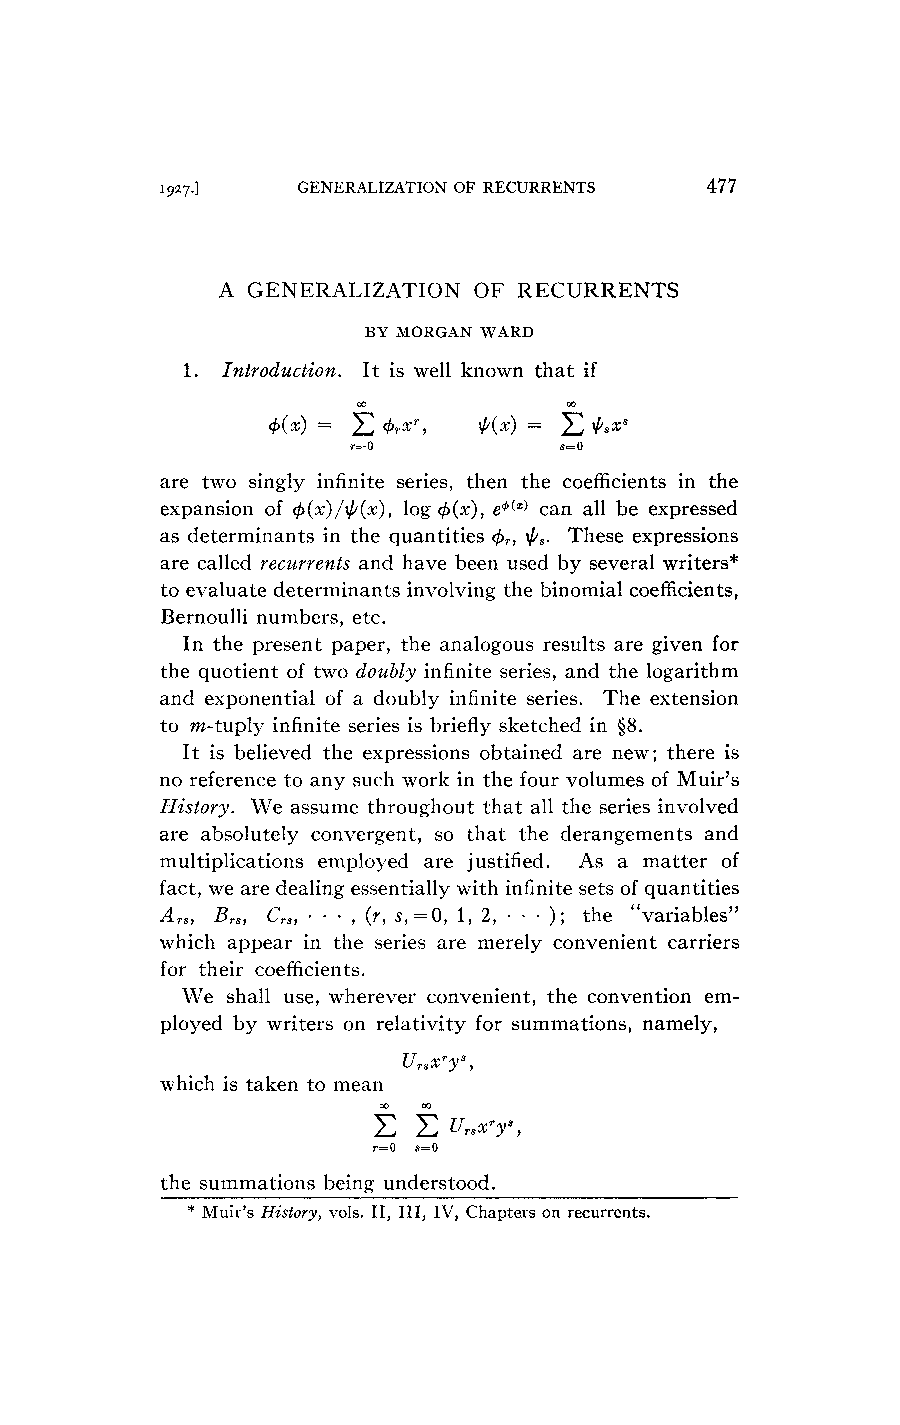
\includepdf[pages={-}]{1927-01 A generalization of recurrents.pdf}
	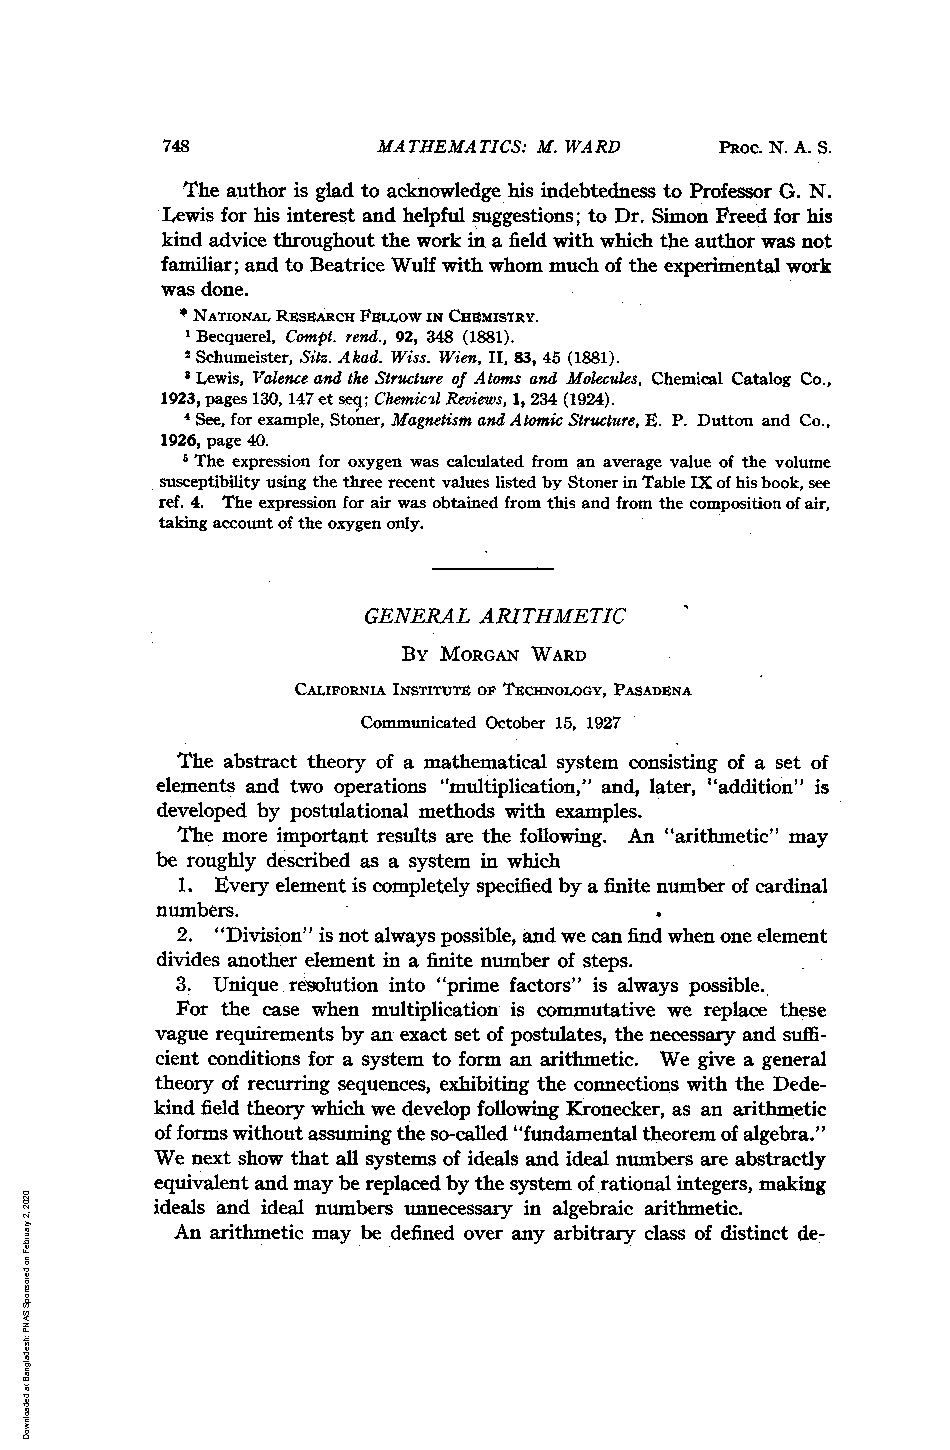
\includepdf[pages={-}]{1927-02 General Arithmetic.pdf}
	\chapter{1928}
	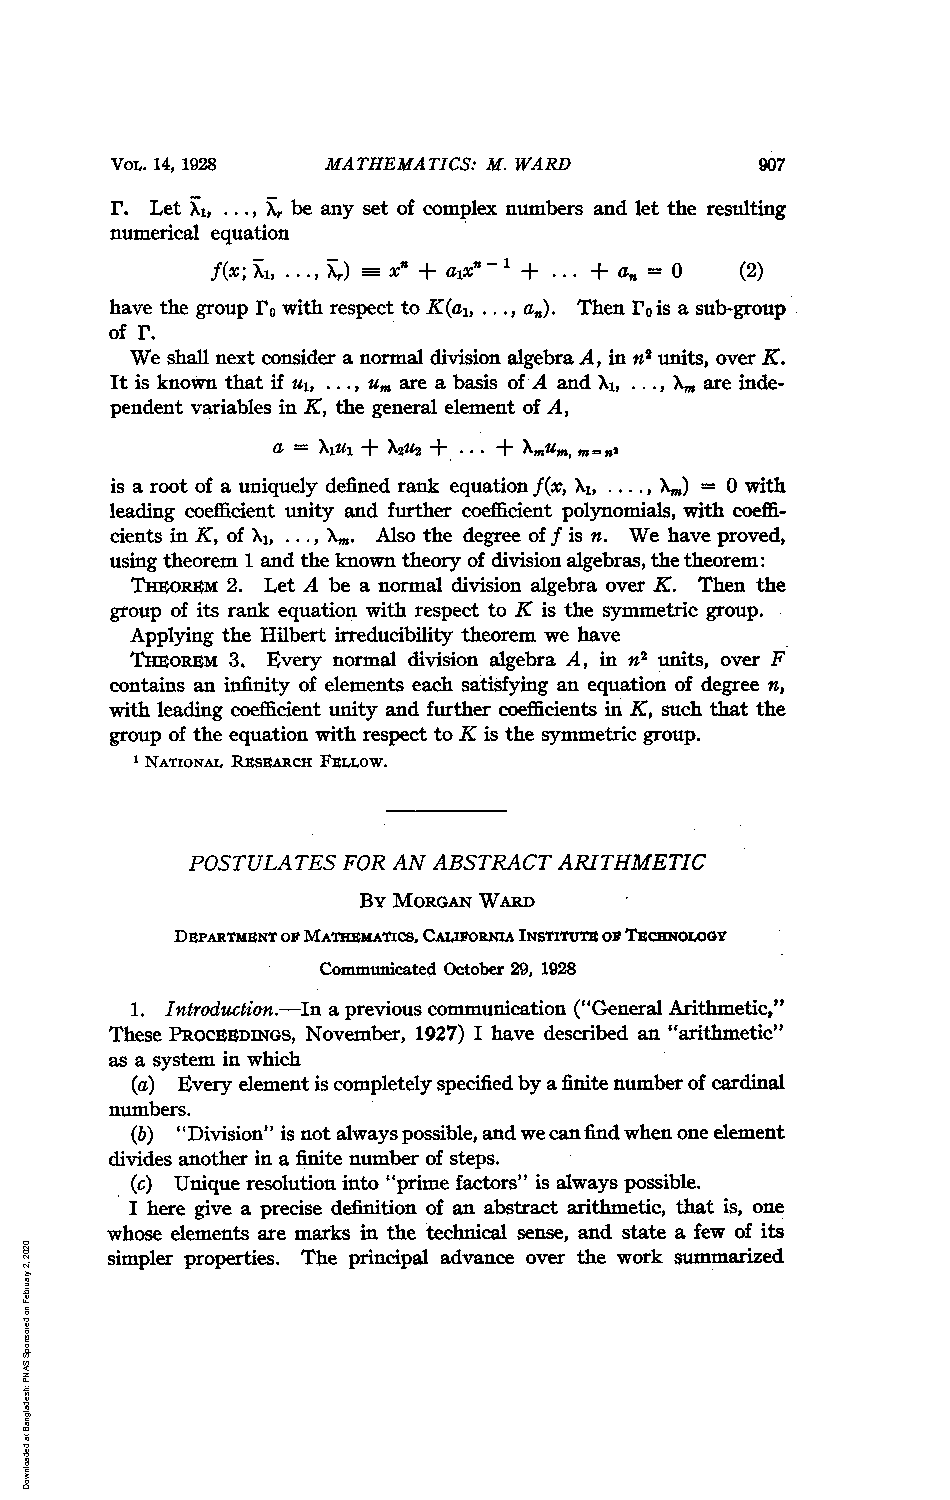
\includepdf[pages={-}]{1928-01 Postulates for an Abstract Arithmetic.pdf}
	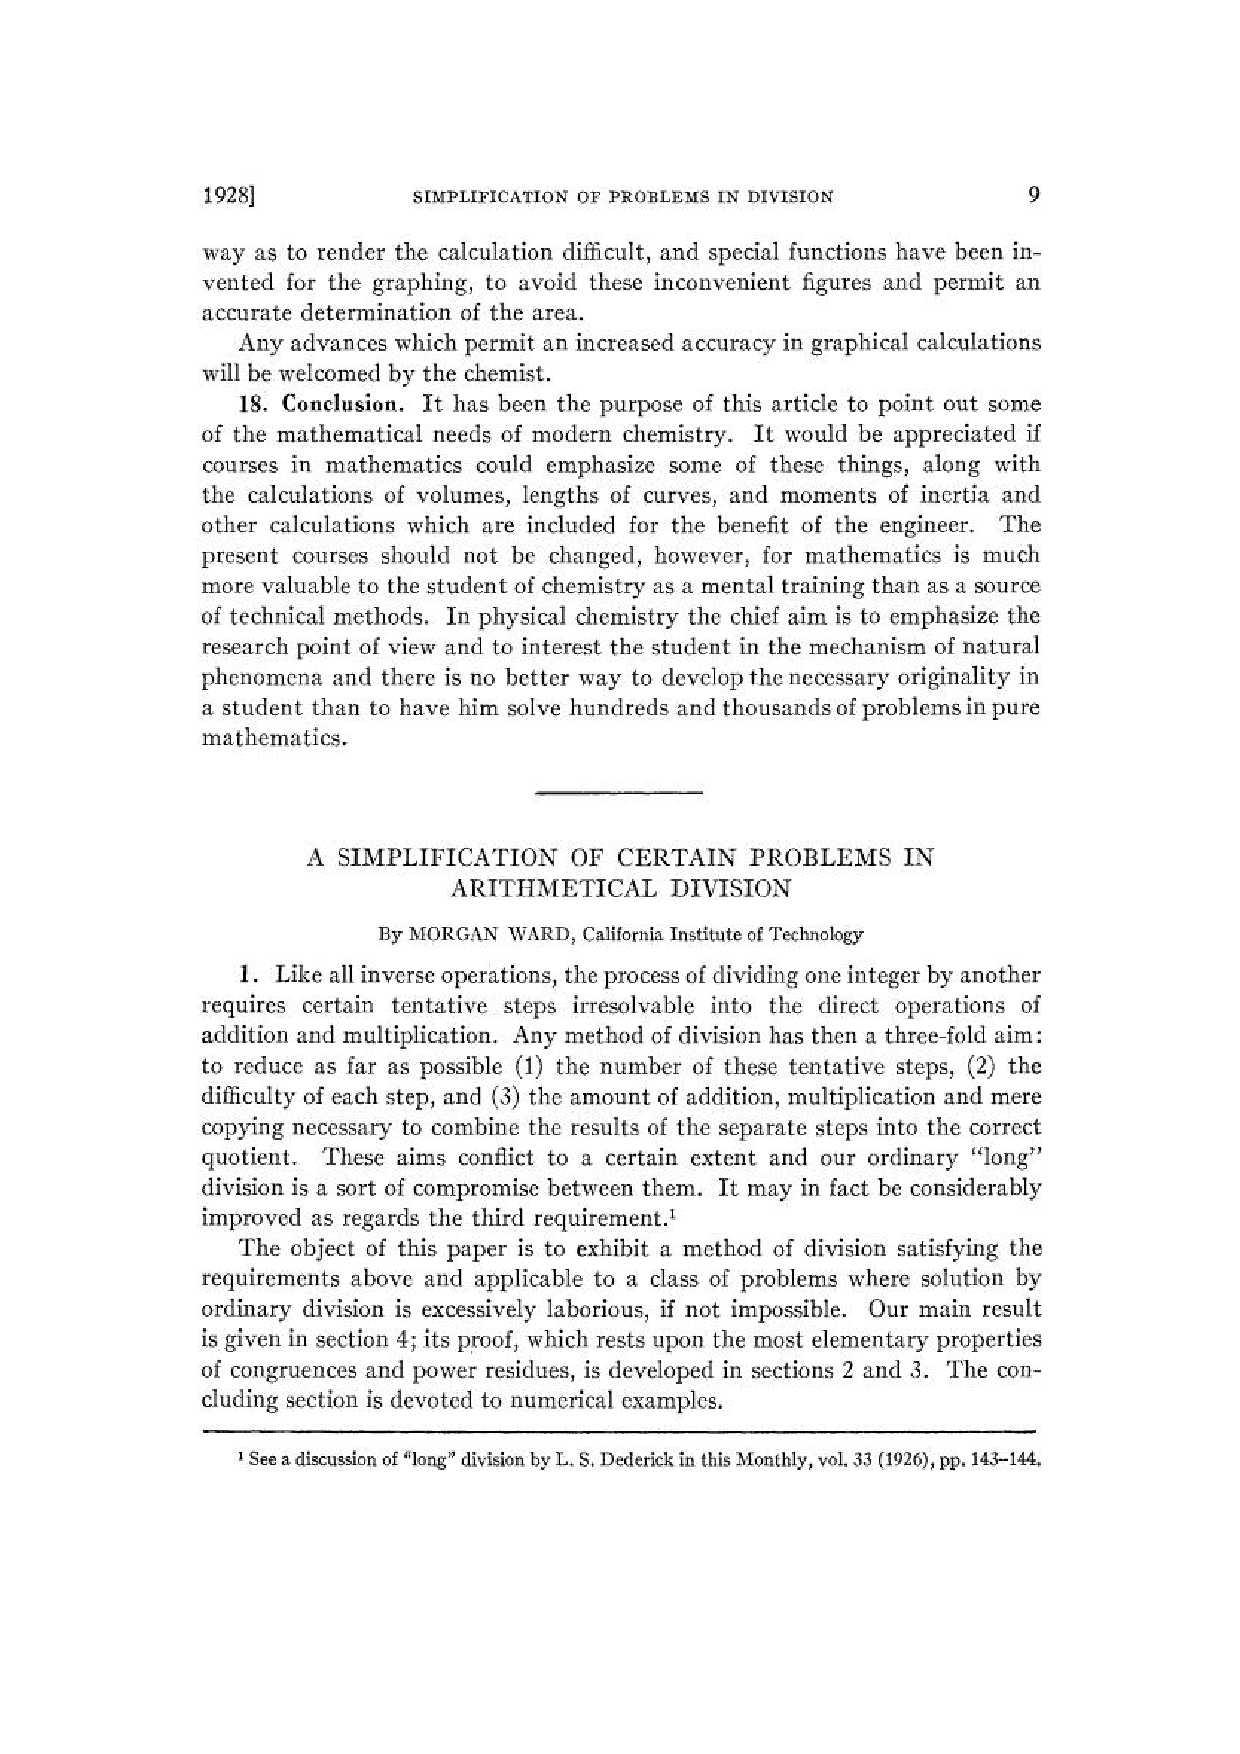
\includepdf[pages={-}]{1928-02 A Simplification of Certain Problems in Arithmetical Division.pdf}
	\chapter{1929}
	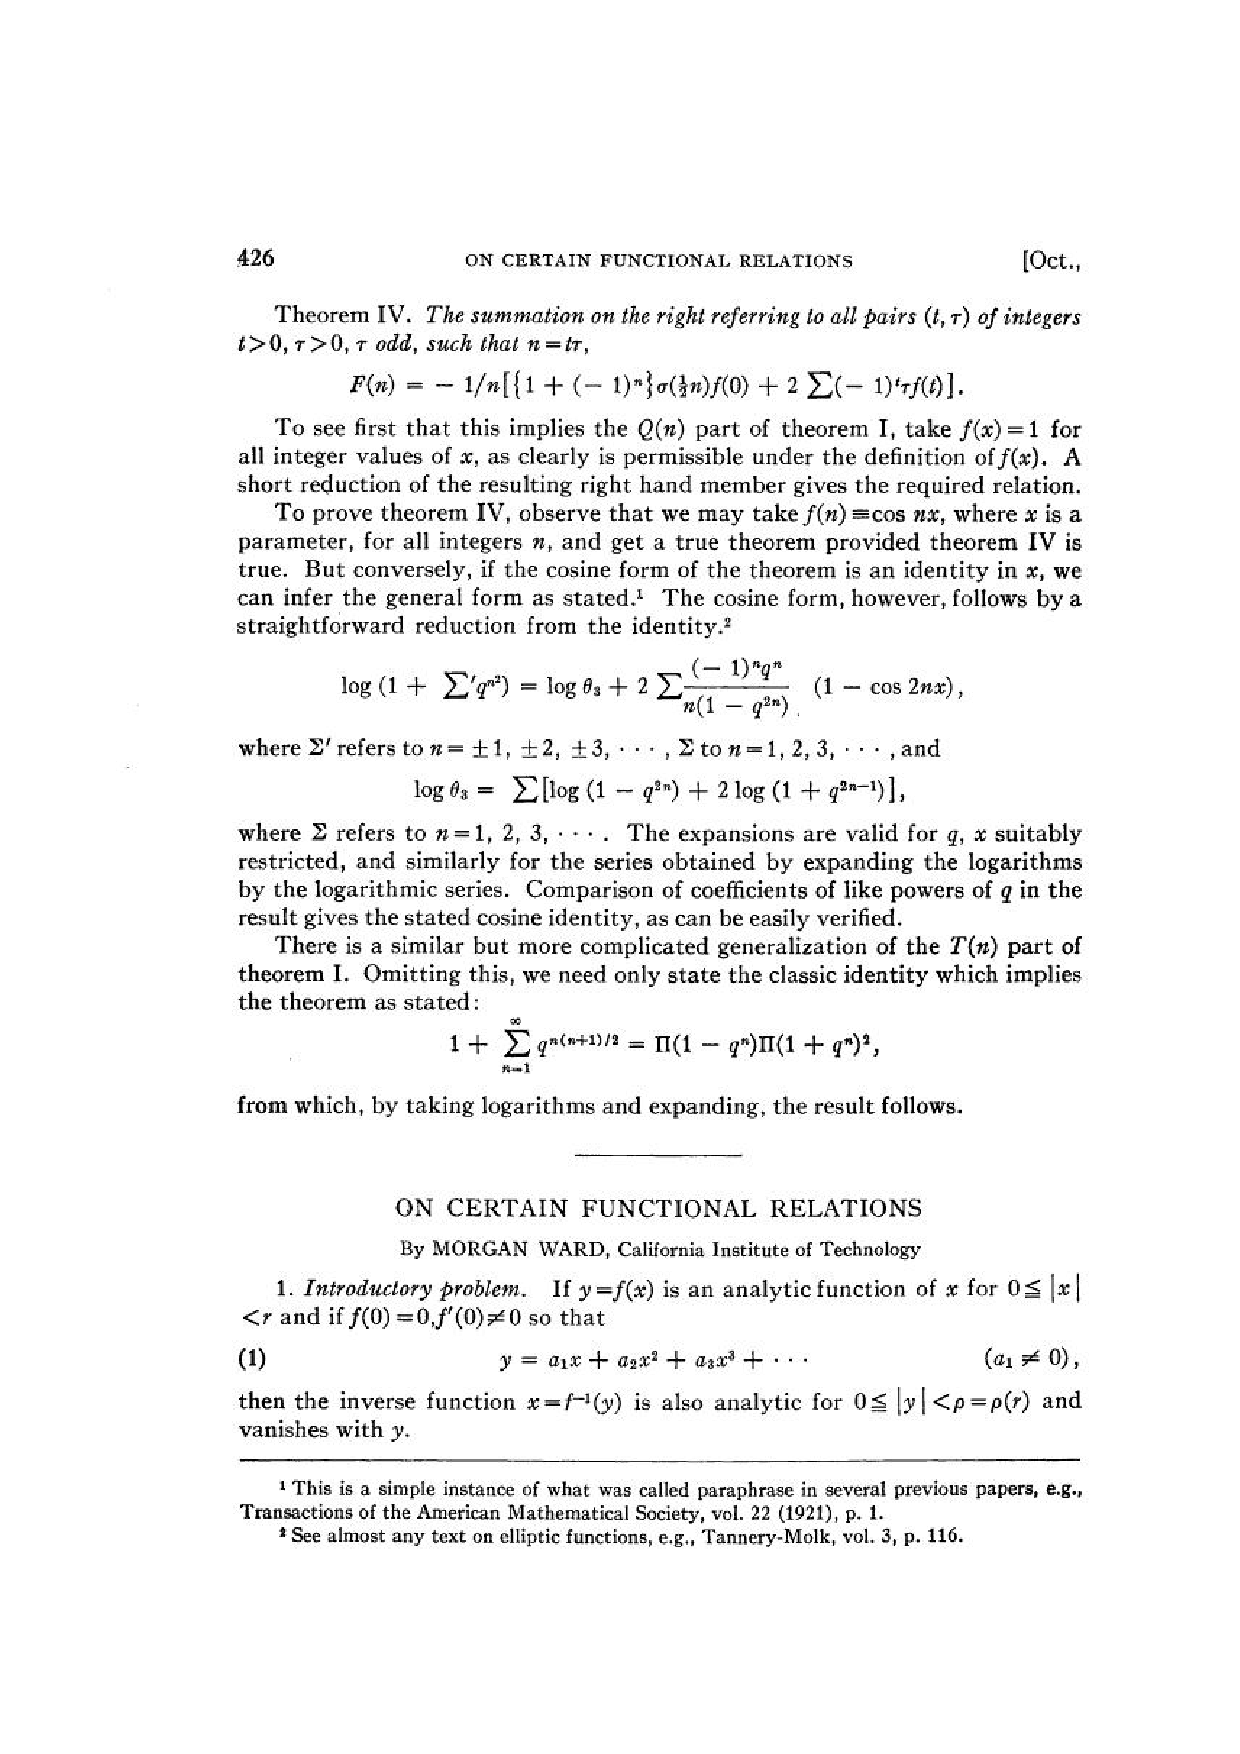
\includepdf[pages={-}]{1929-01 On Certain Functional Relations.pdf}
	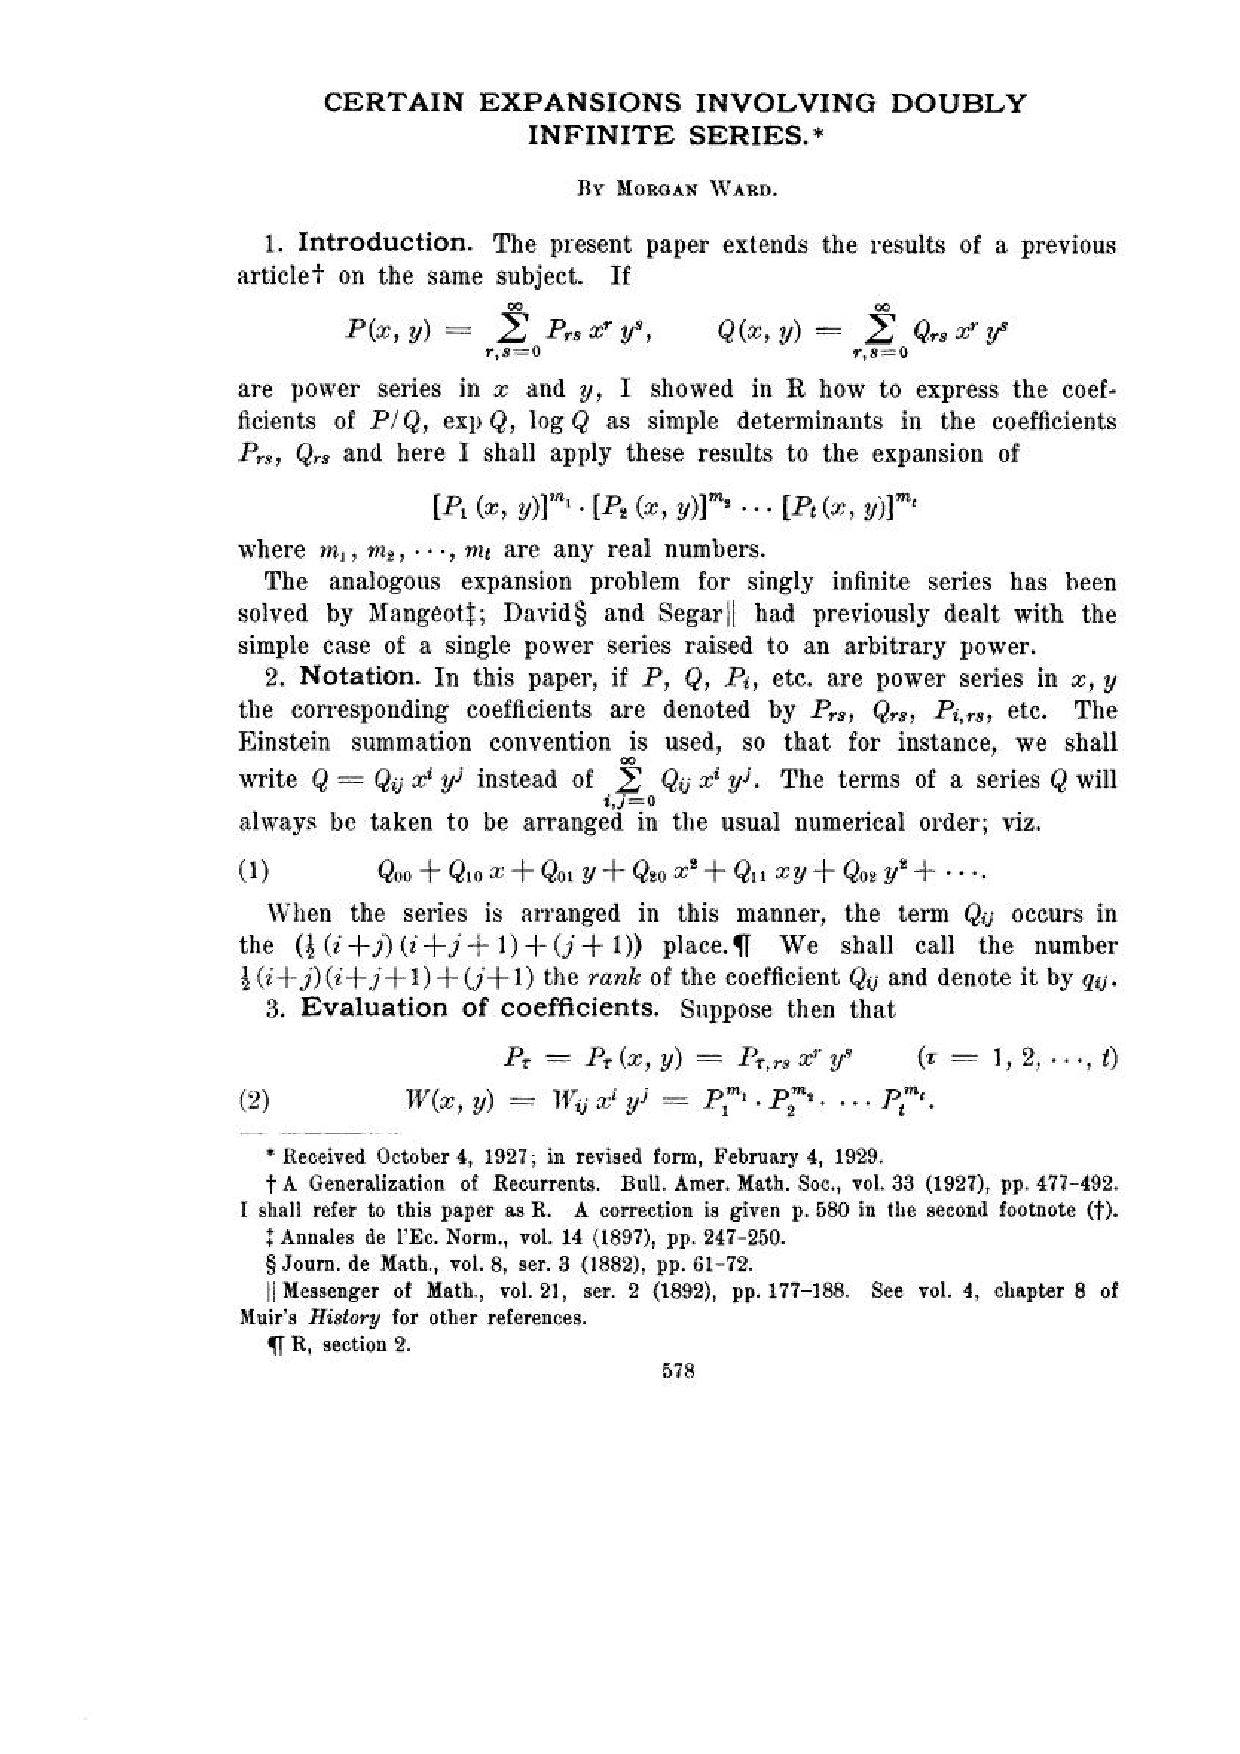
\includepdf[pages={-}]{1929-02 Certain Expansions Involving Doubly Infinite Series.pdf}
	\chapter{1930}
	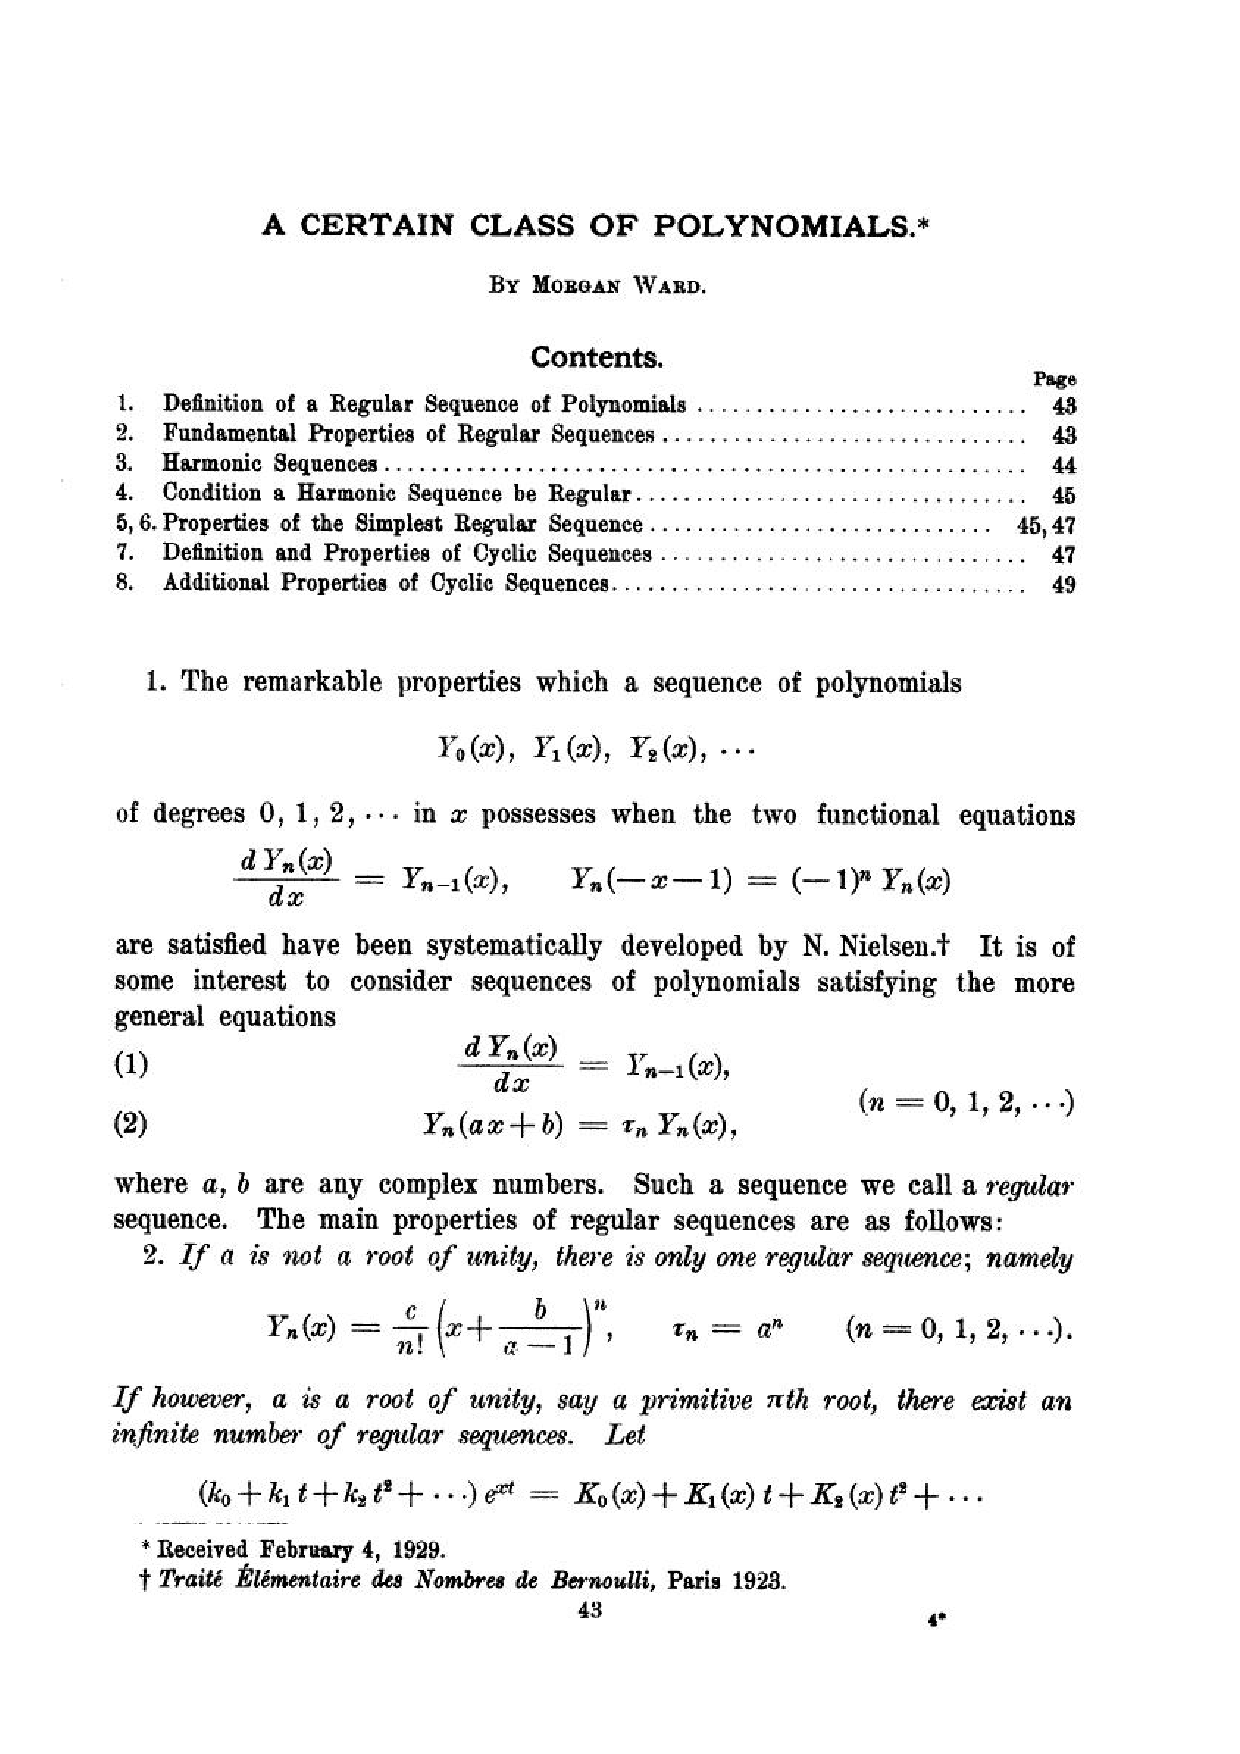
\includepdf[pages={-}]{1930-01 A Certain Class of Polynomials.pdf}
	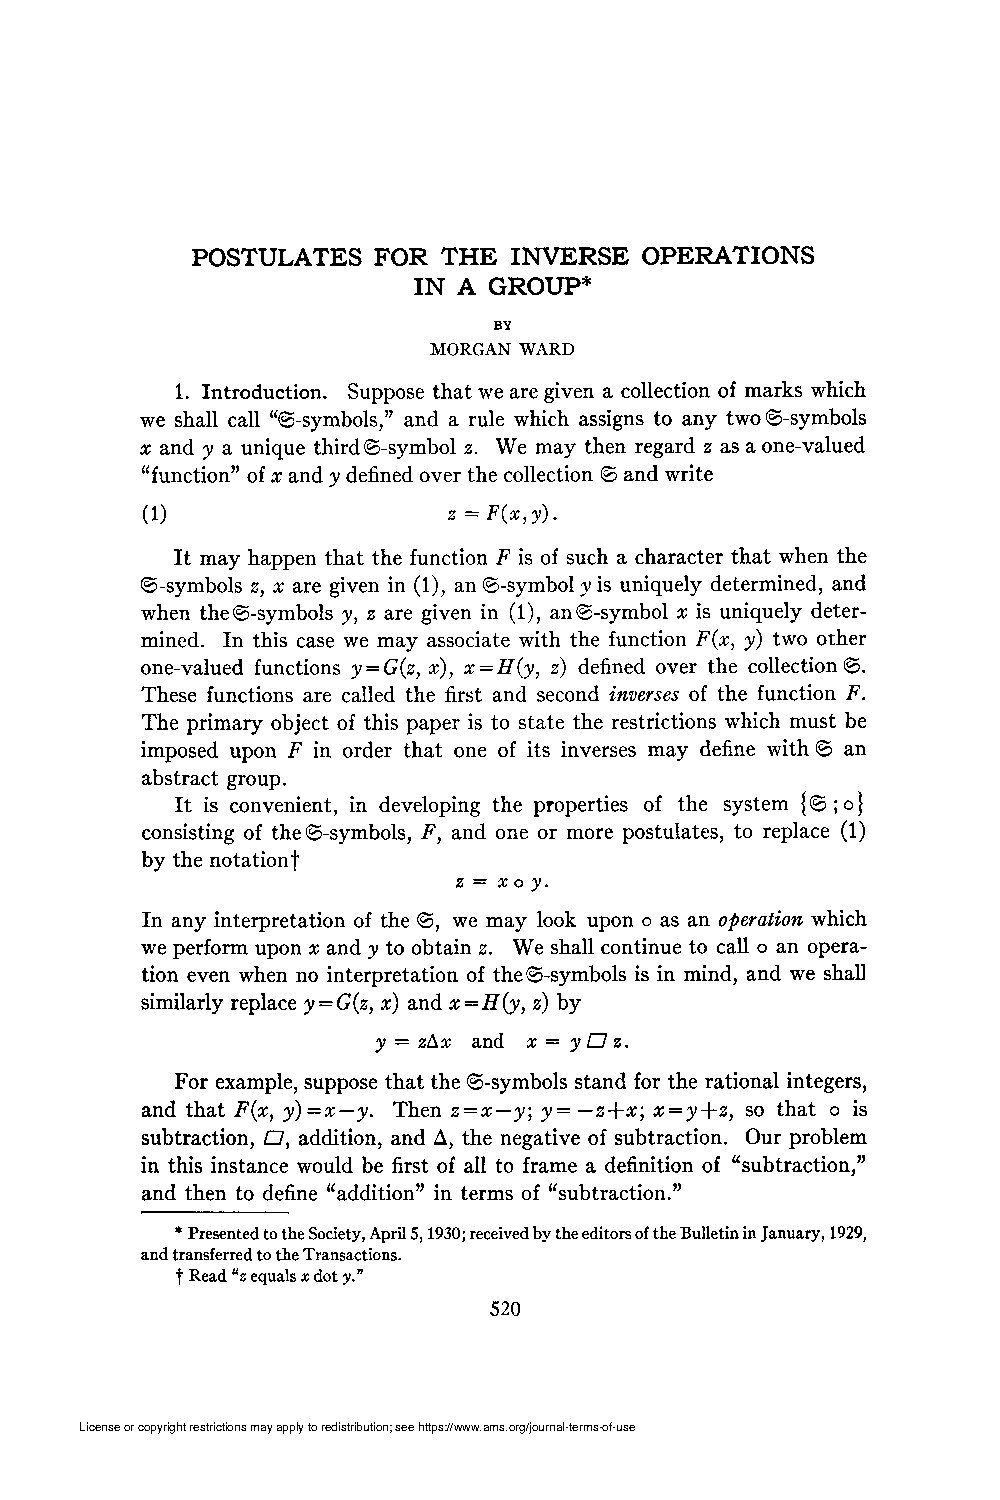
\includepdf[pages={-}]{1930-04 Postulates for the inverse operations in a group.pdf}
	\chapter{1931}
	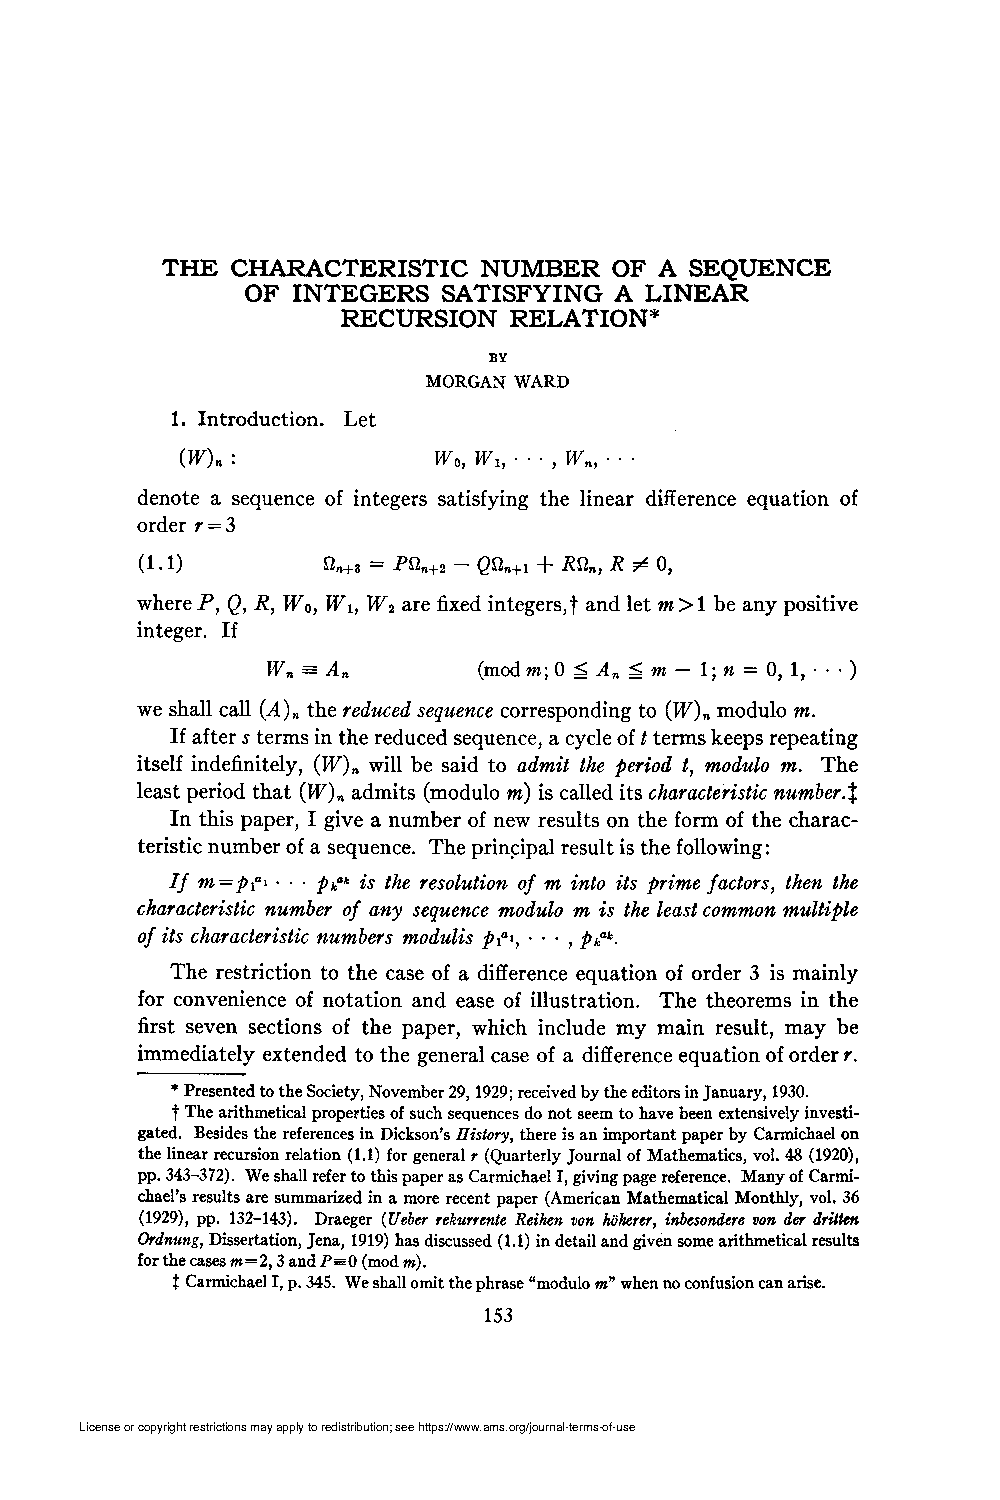
\includepdf[pages={-}]{1931-01 The characteristic number of a sequence of integers satisfying a linear recursion relation.pdf}
	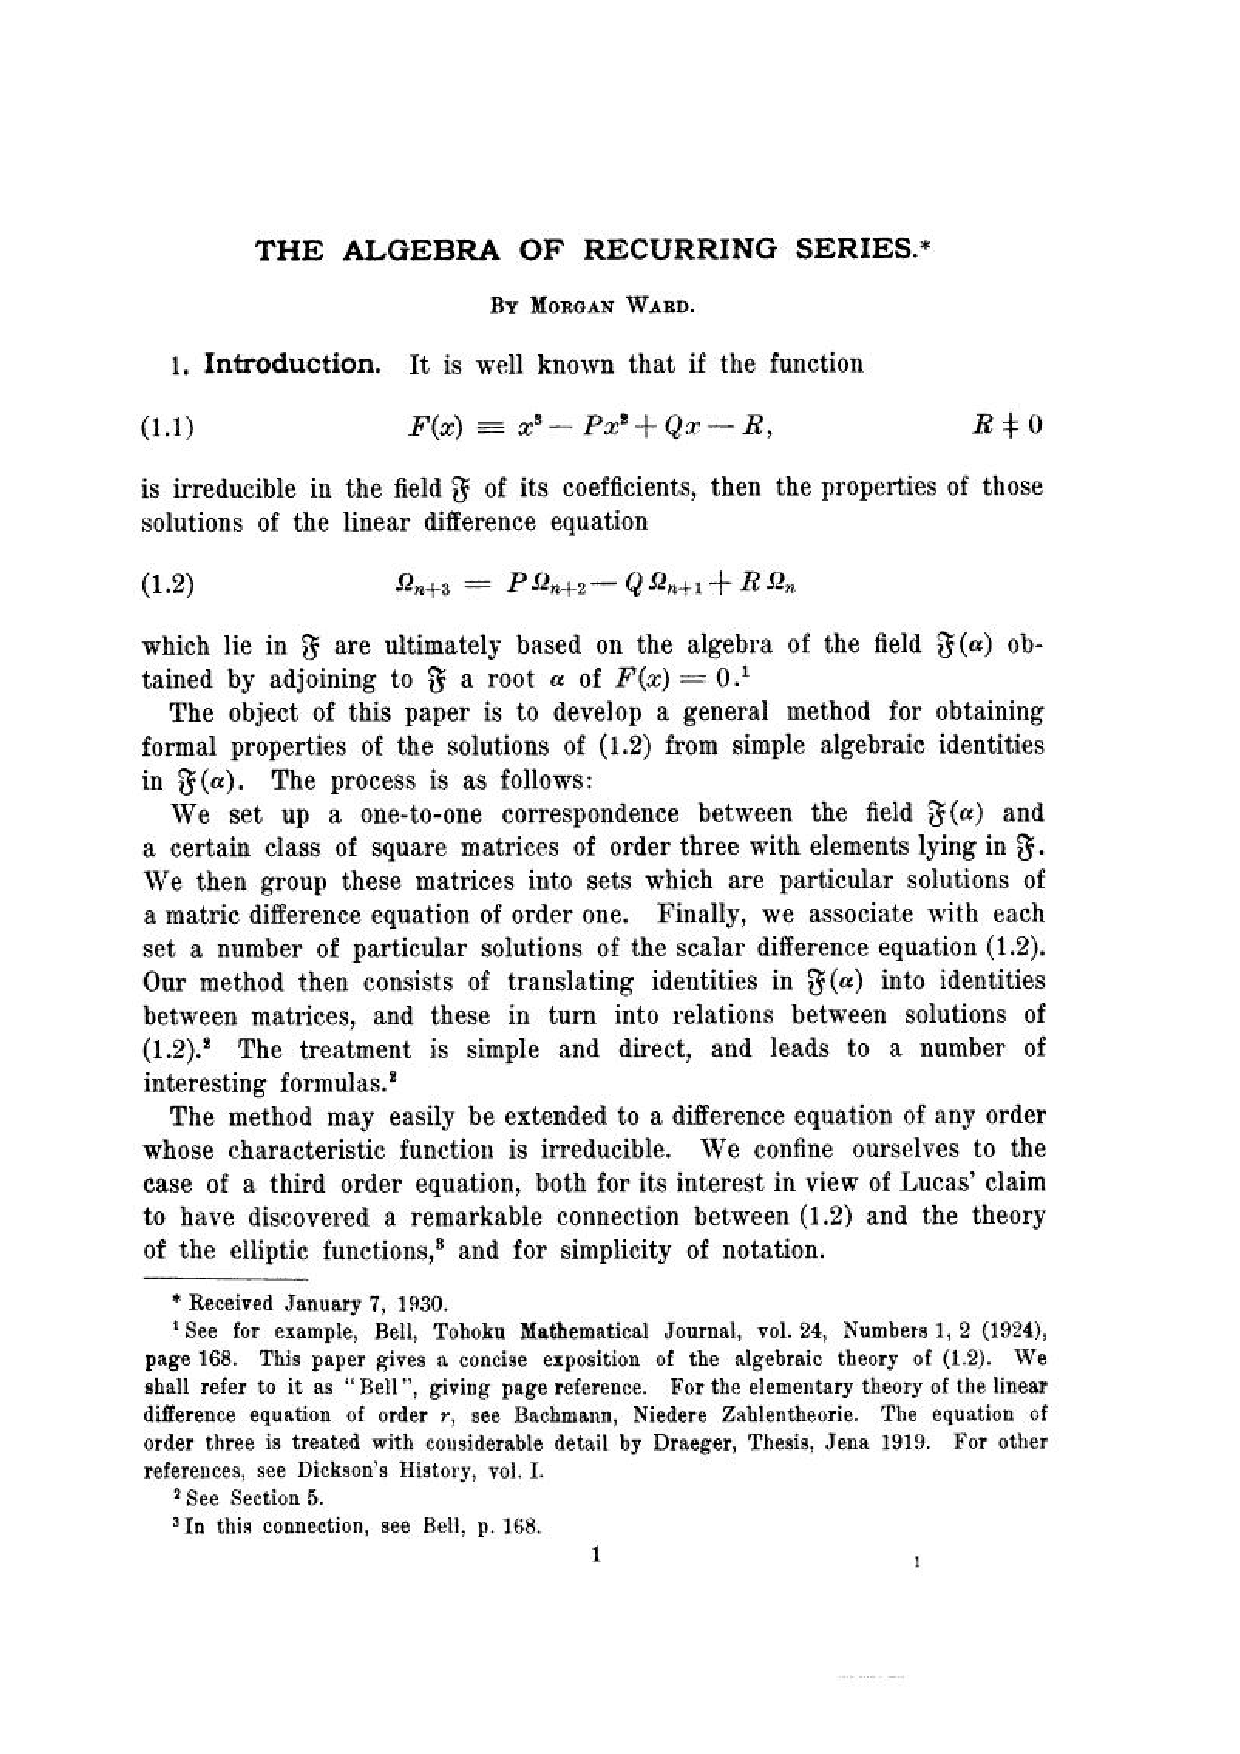
\includepdf[pages={-}]{1931-02 The Algebra of Recurring Series.pdf}
	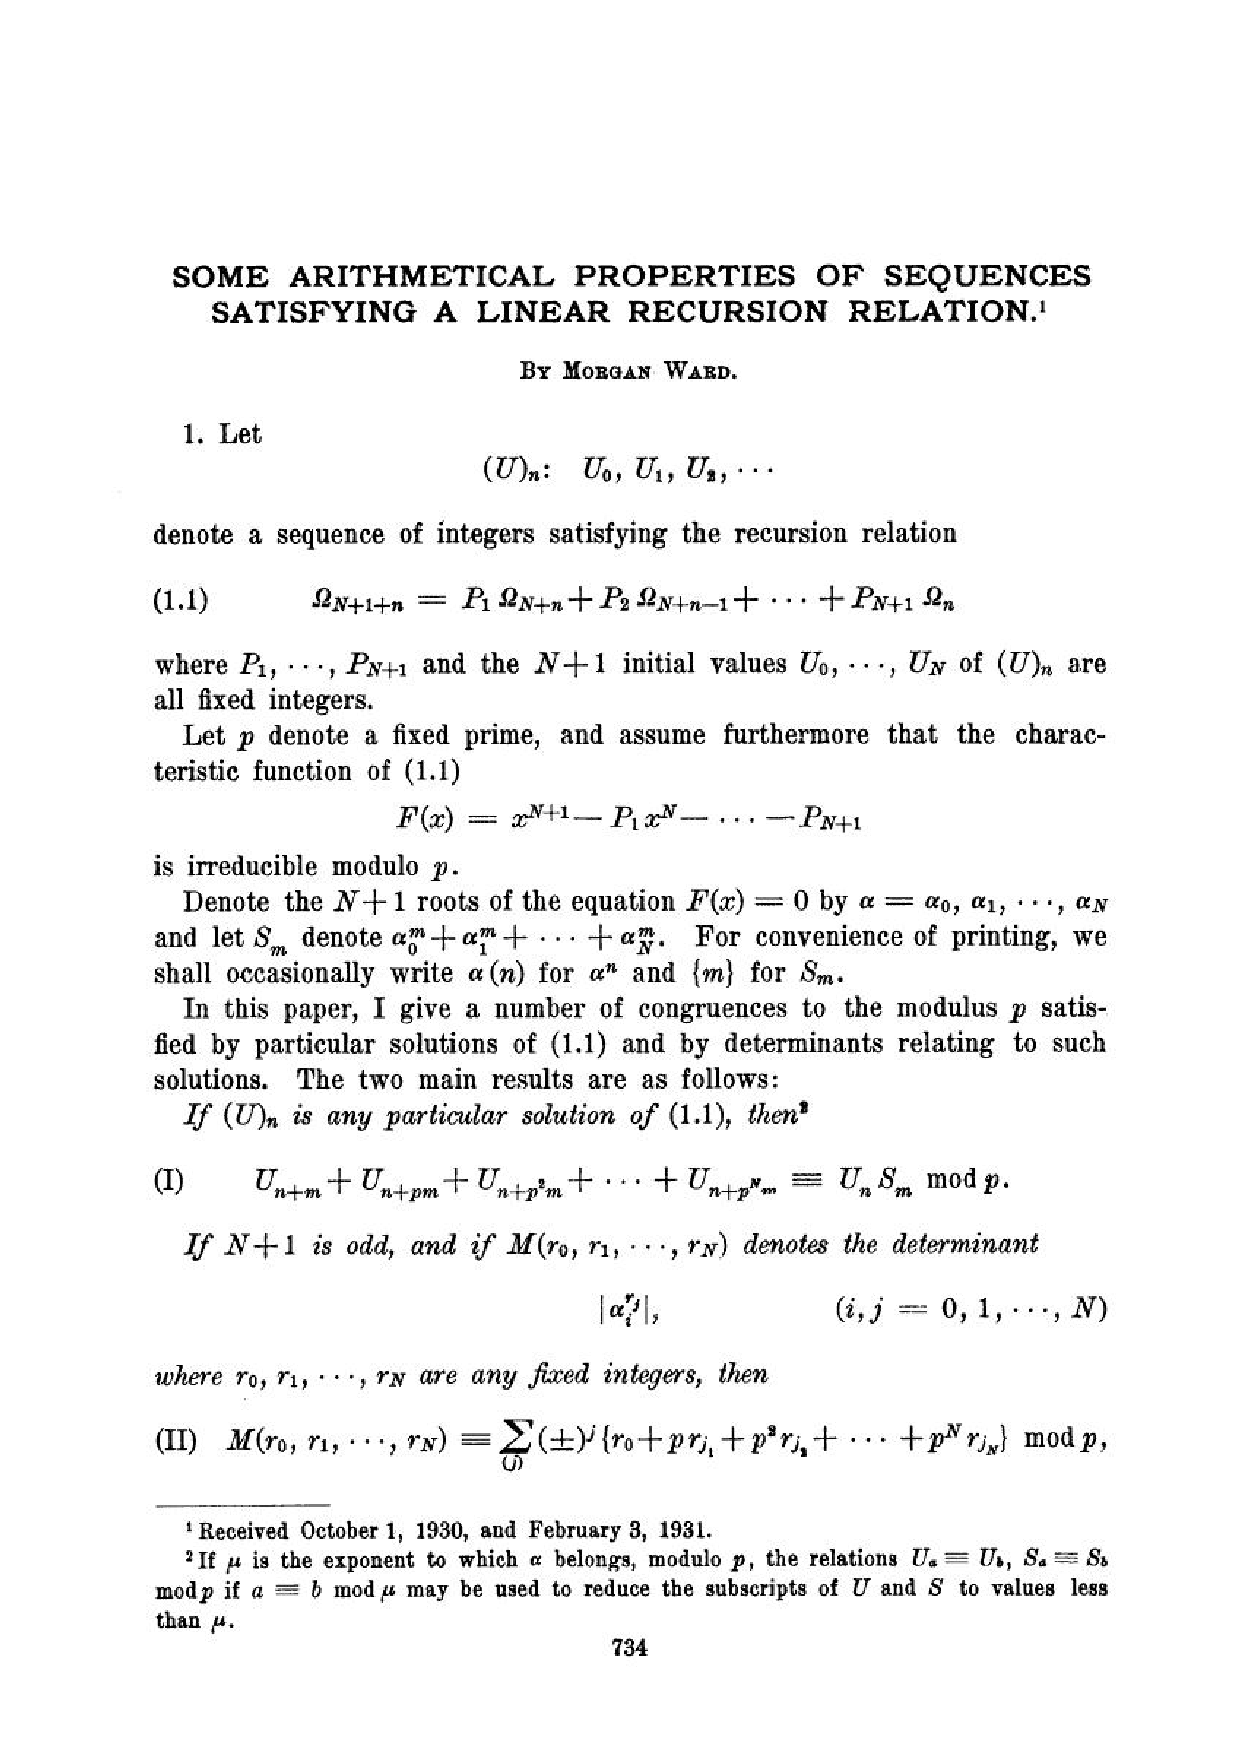
\includepdf[pages={-}]{1931-03 Some Arithmetical Properties of Sequences Satisfying a Linear Recursion Relation.pdf}
	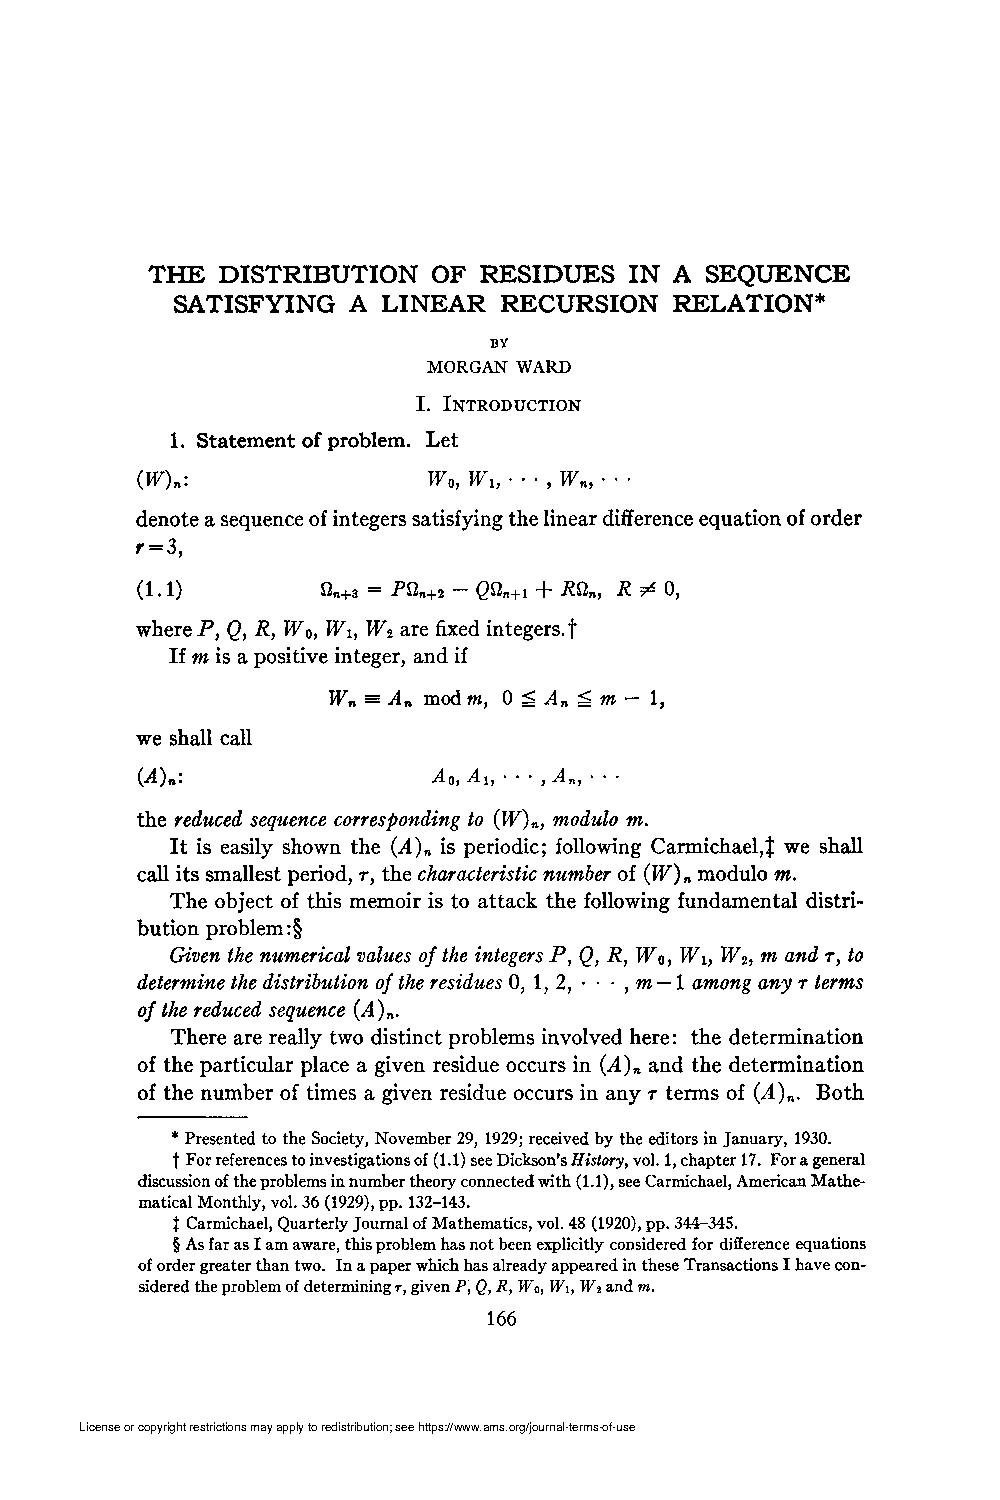
\includepdf[pages={-}]{1931-04 The distribution of residues in a sequence satisfying a linear recursion relation.pdf}
	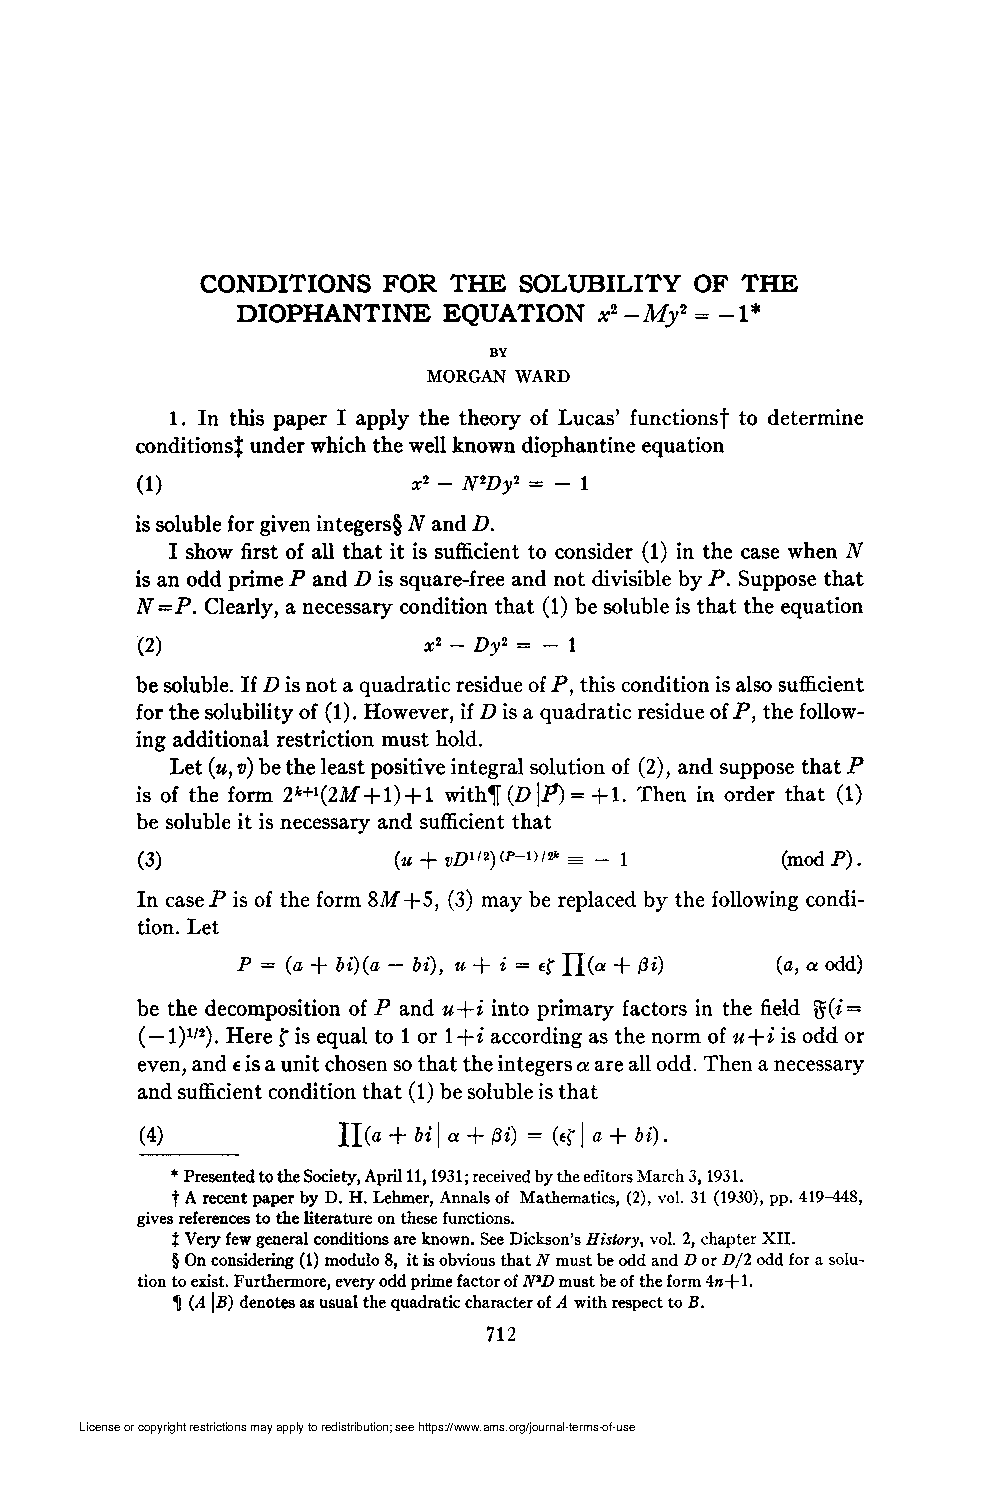
\includepdf[pages={-}]{1931-05 Conditions for the solubility of the Diophantine equation .pdf}
	\chapter{1932}
	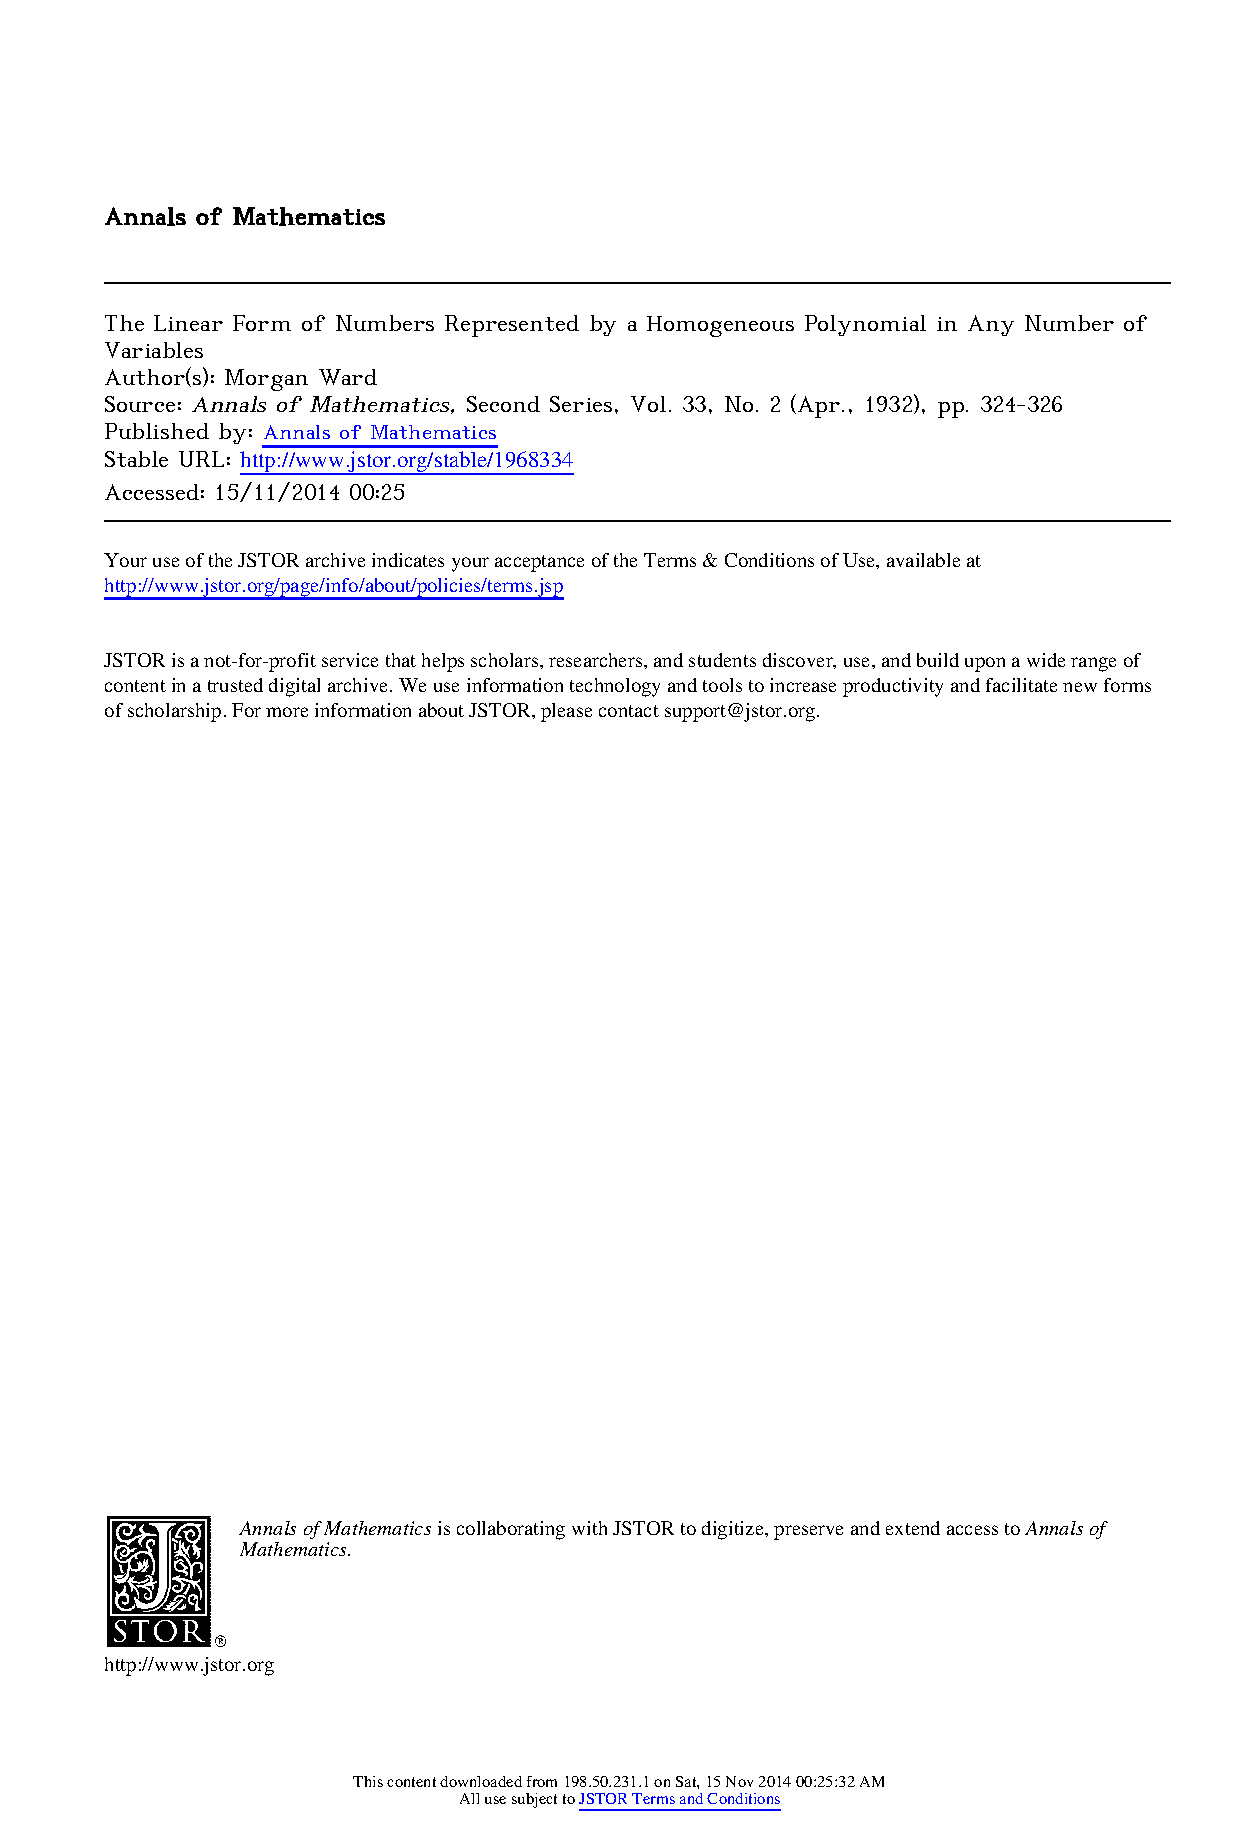
\includepdf[pages={-}]{1932-01 The Linear Form of Numbers Represented by a Homogeneous Polynomial in Any Number of.pdf}
	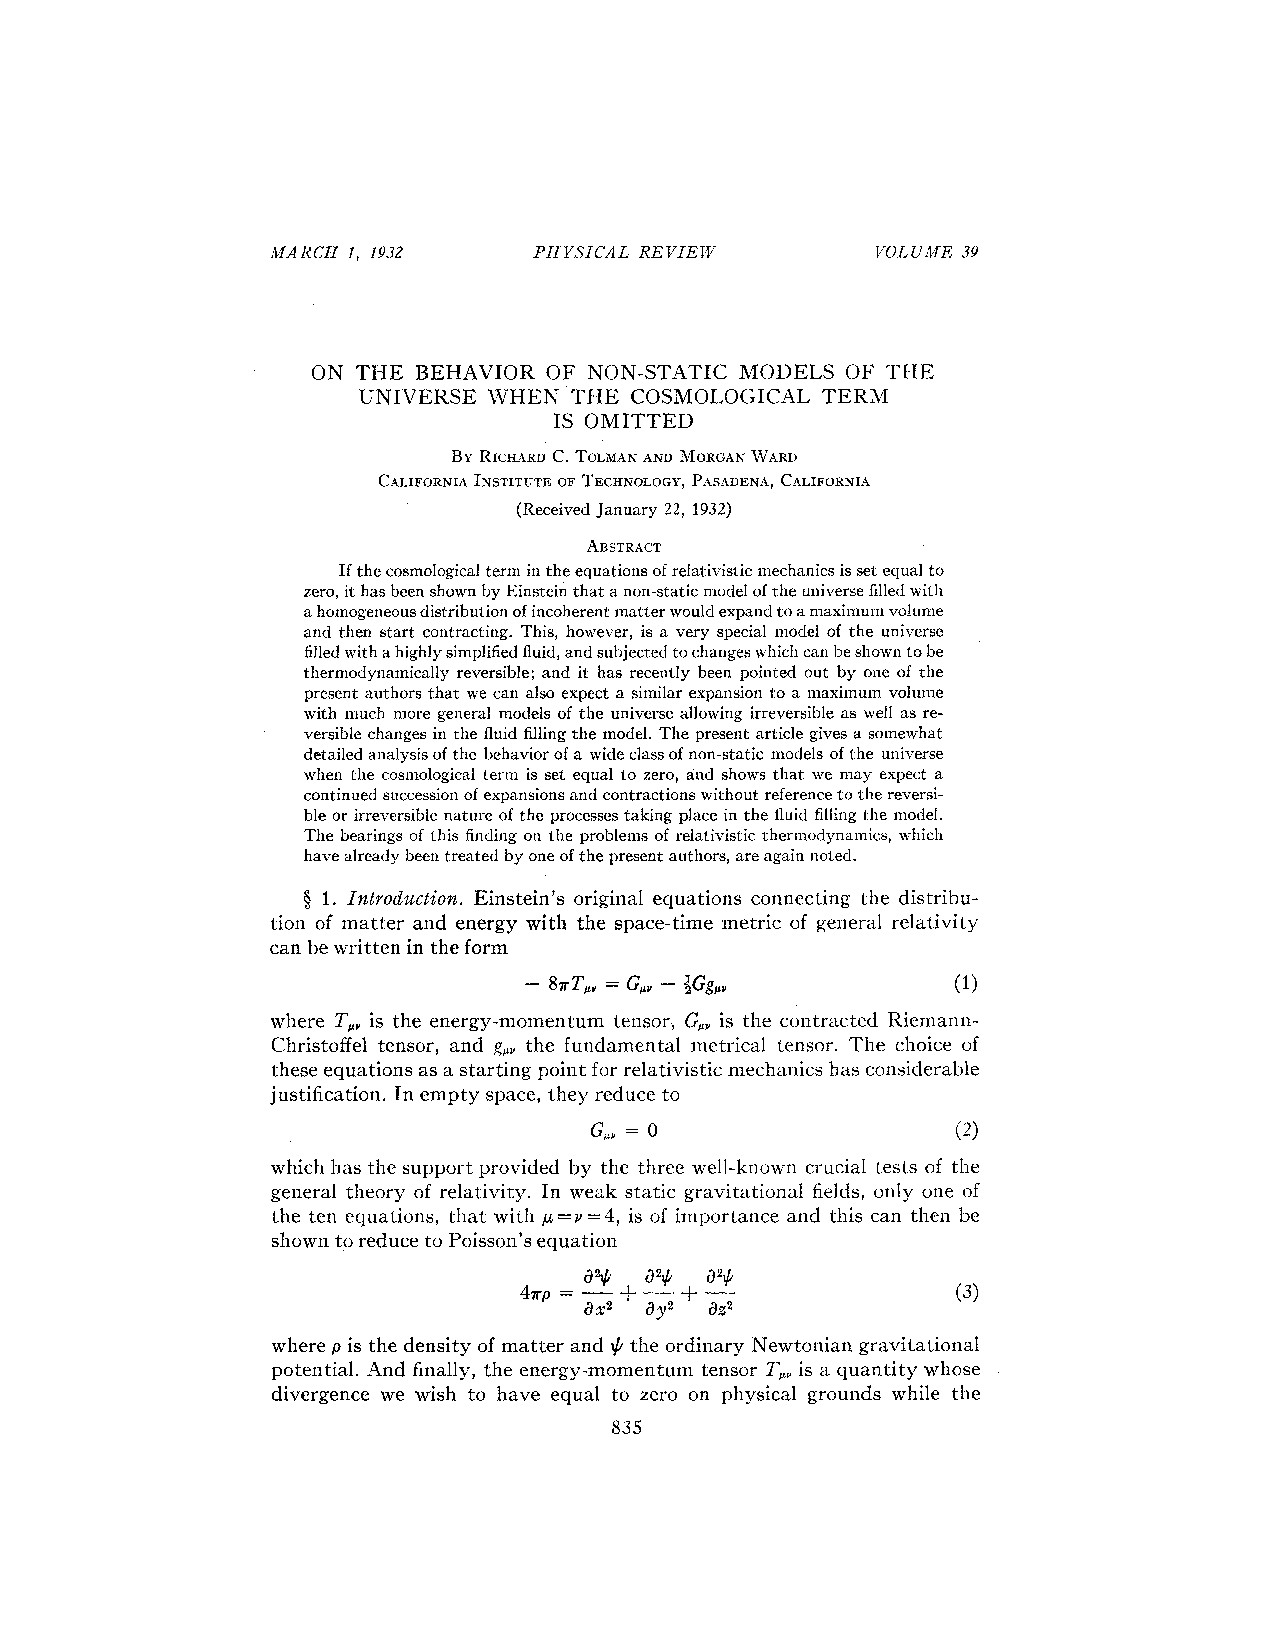
\includepdf[pages={-}]{1932-02 On the behavior of non-static models of the universe when the cosmological term is omitted.pdf}
	\chapter{1933}
	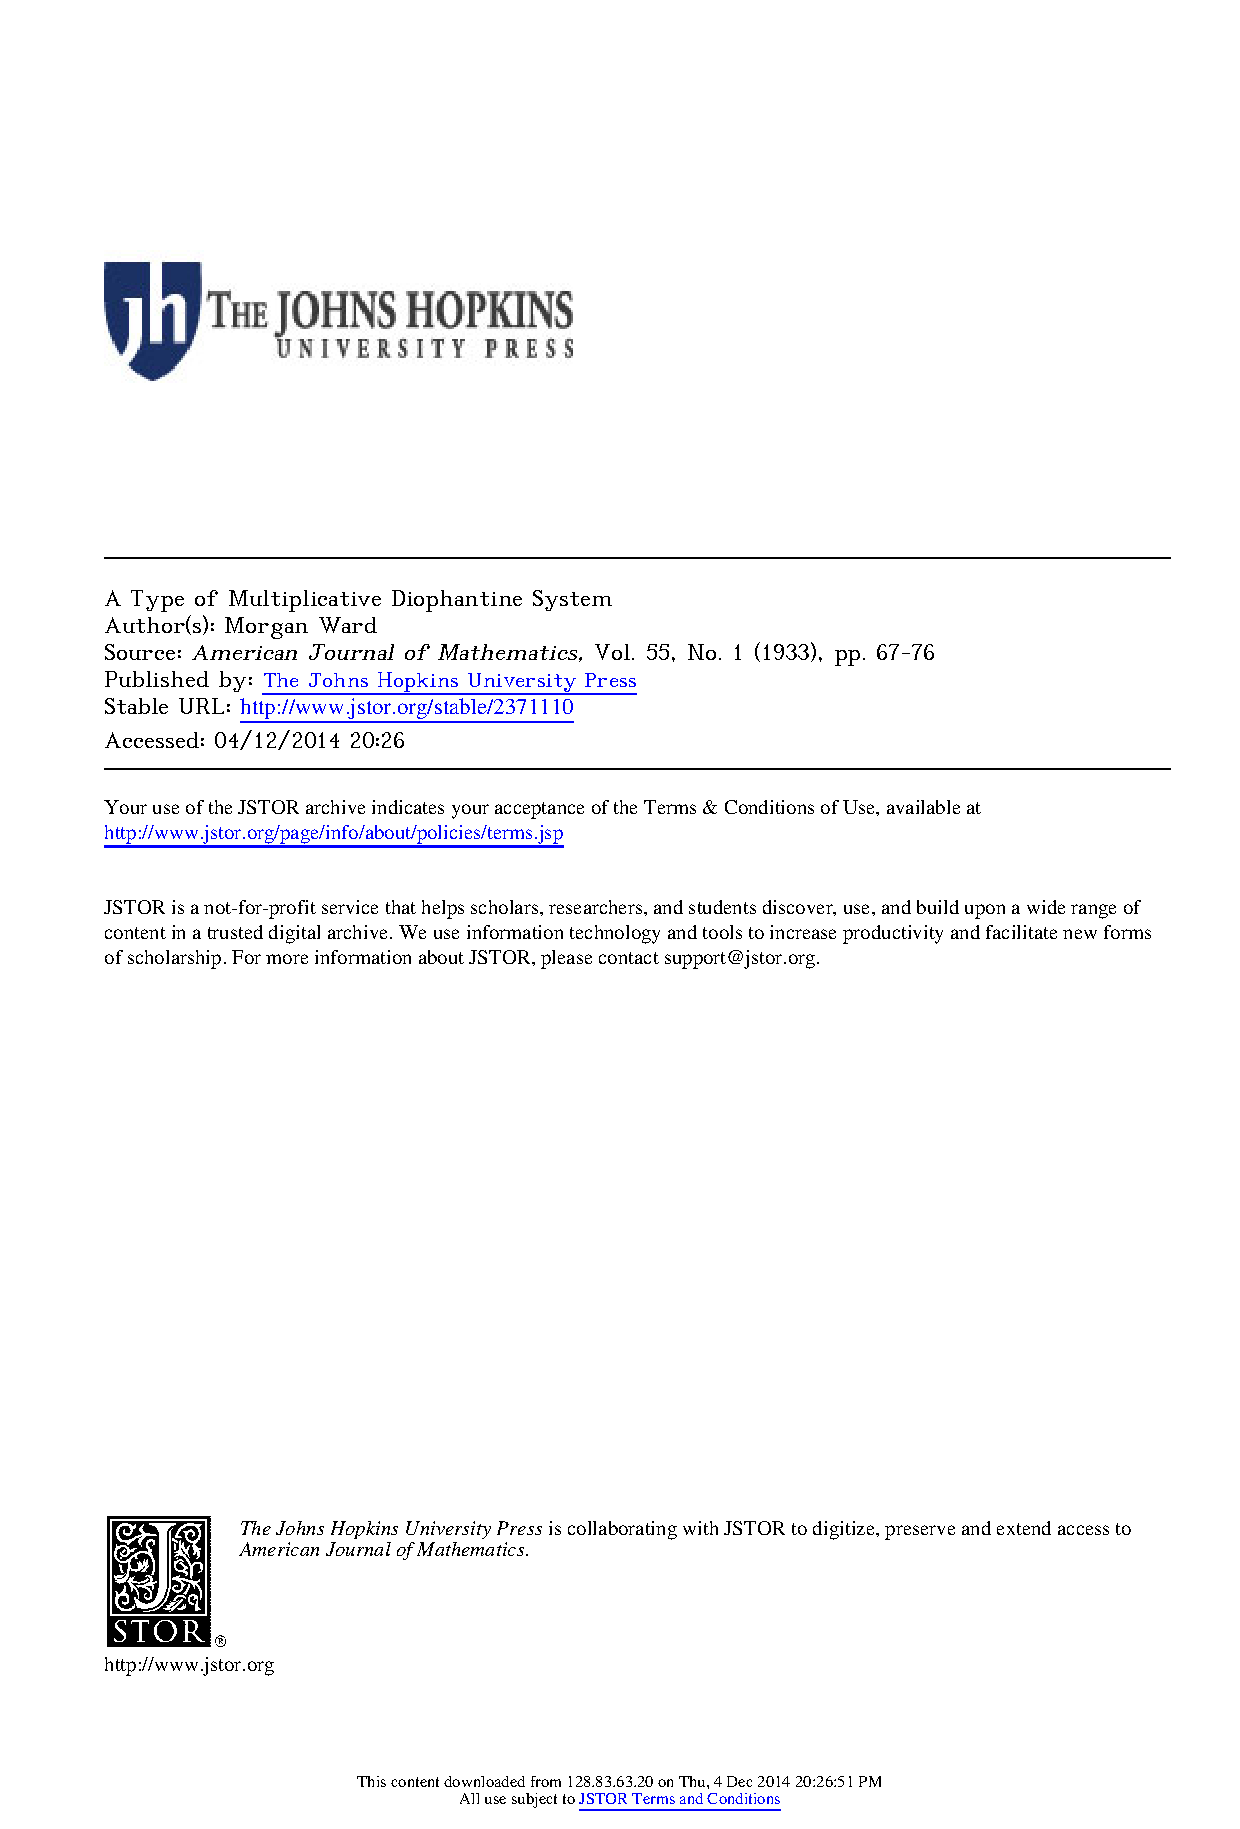
\includepdf[pages={-}]{1933-01 A Type of Multiplicative Diophantine System.pdf}
	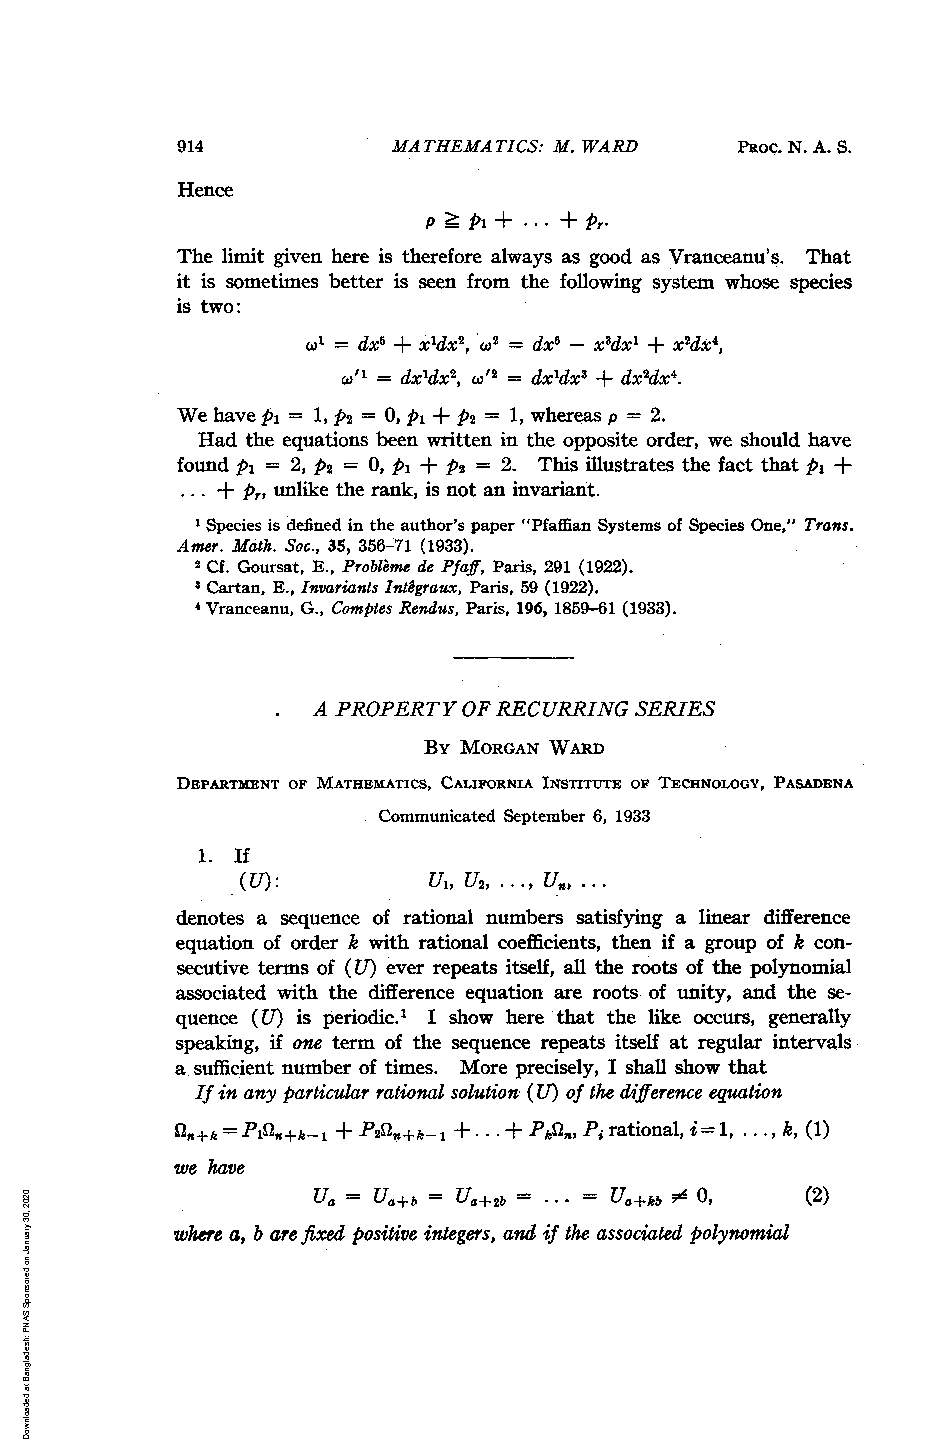
\includepdf[pages={-}]{1933-02 A property of recurring series.pdf}
	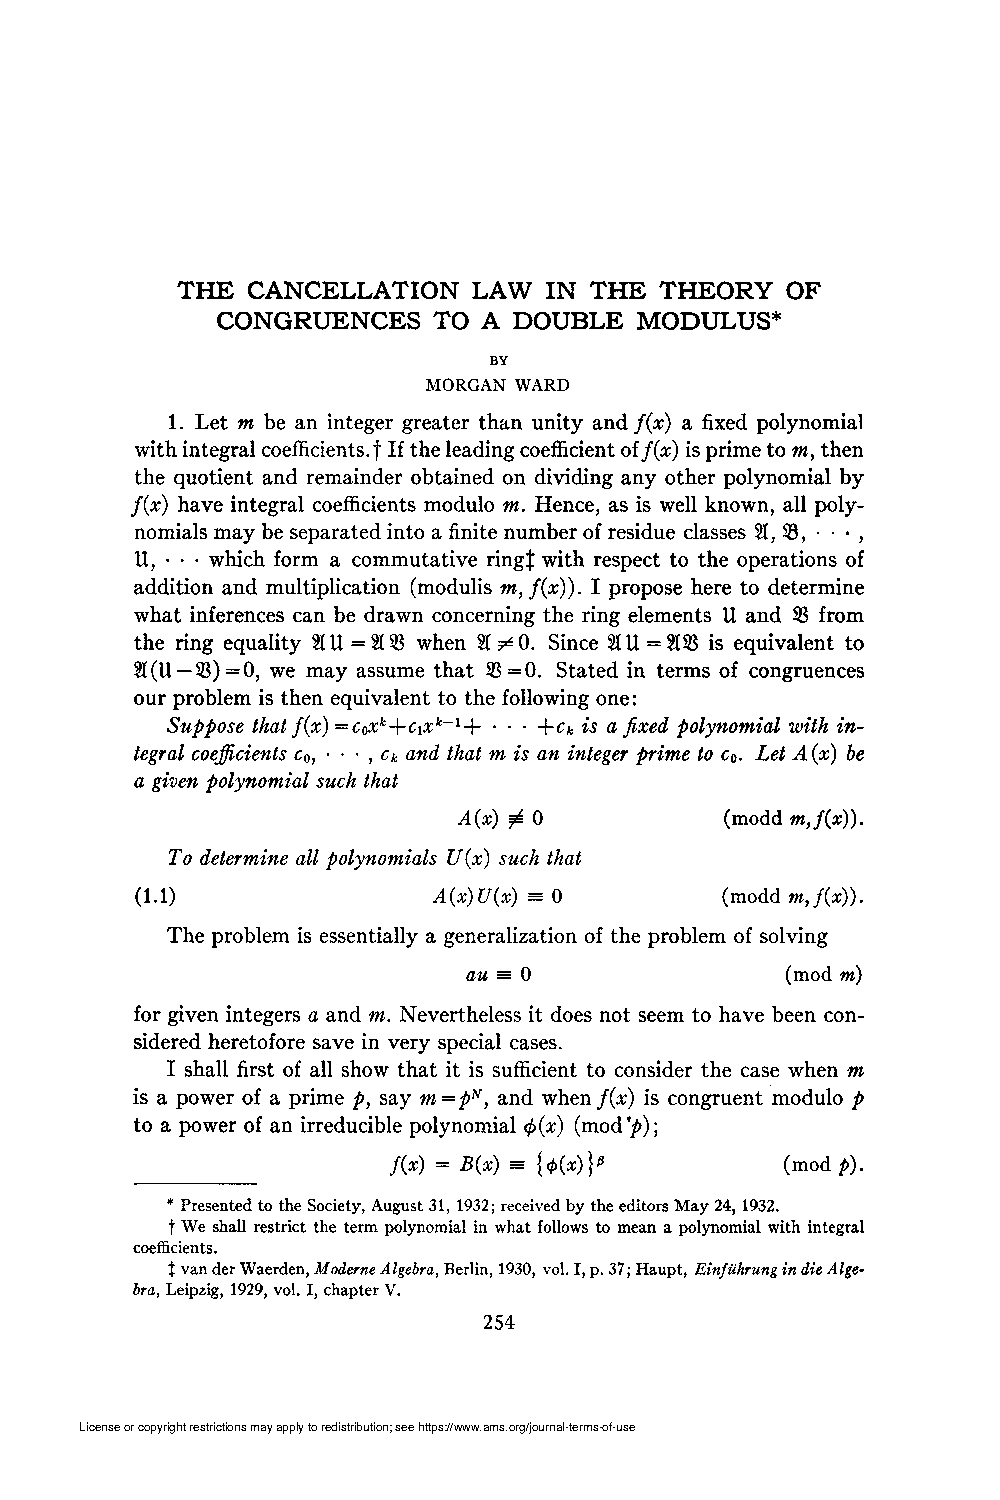
\includepdf[pages={-}]{1933-03 The cancellation law in the theory of congruences to a double modulus.pdf}
	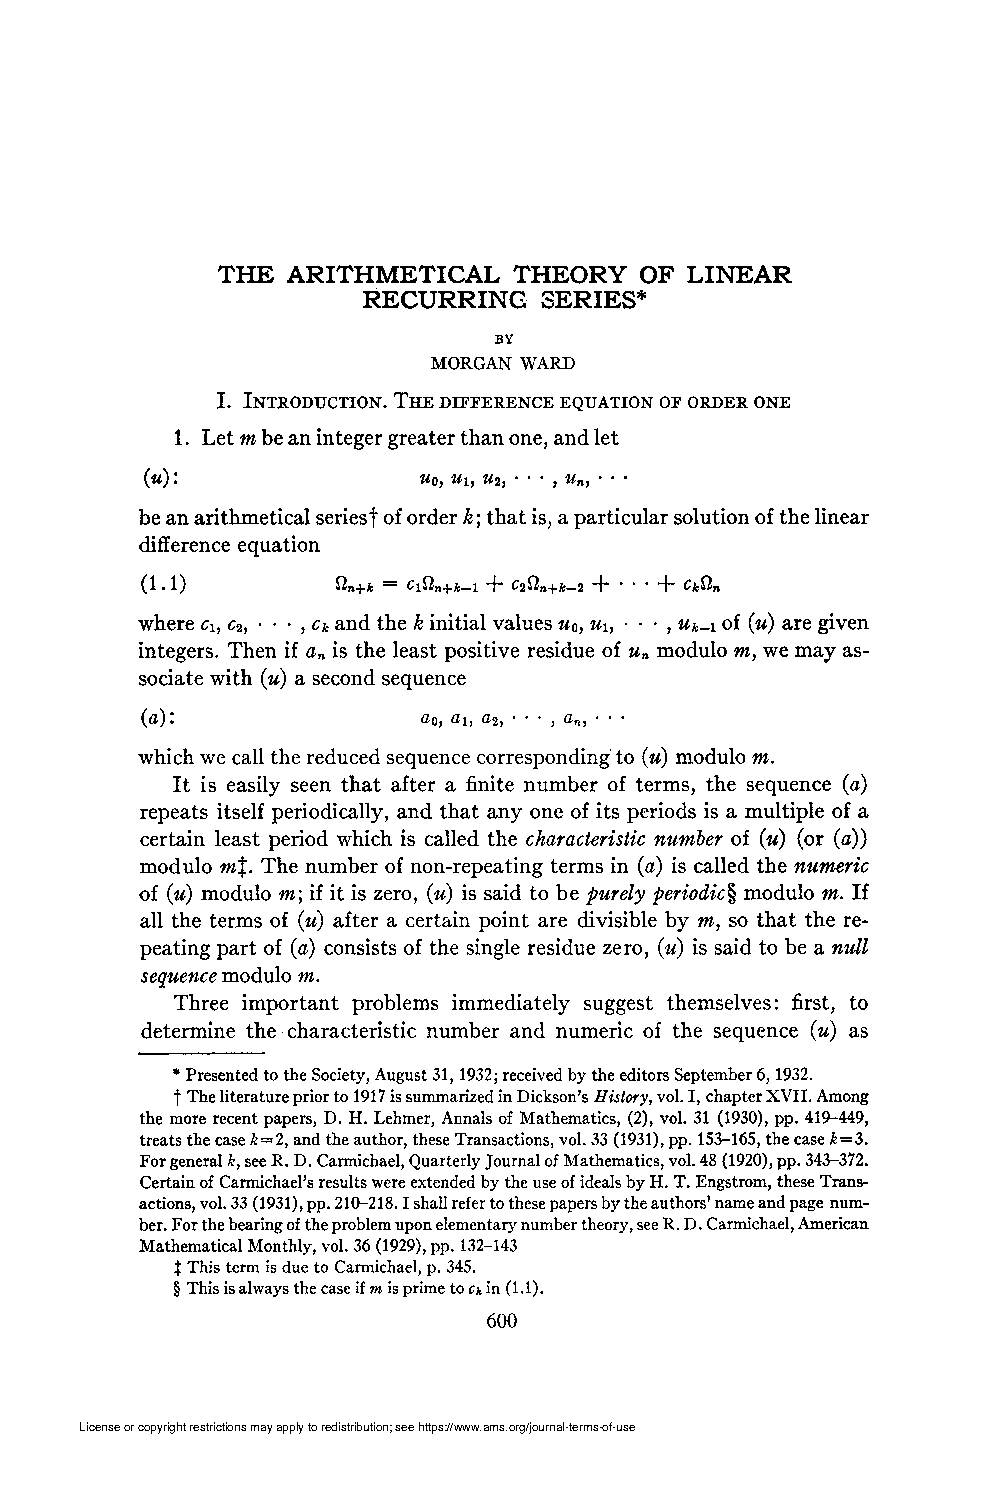
\includepdf[pages={-}]{1933-04 The arithmetical theory of linear recurring series.pdf}
	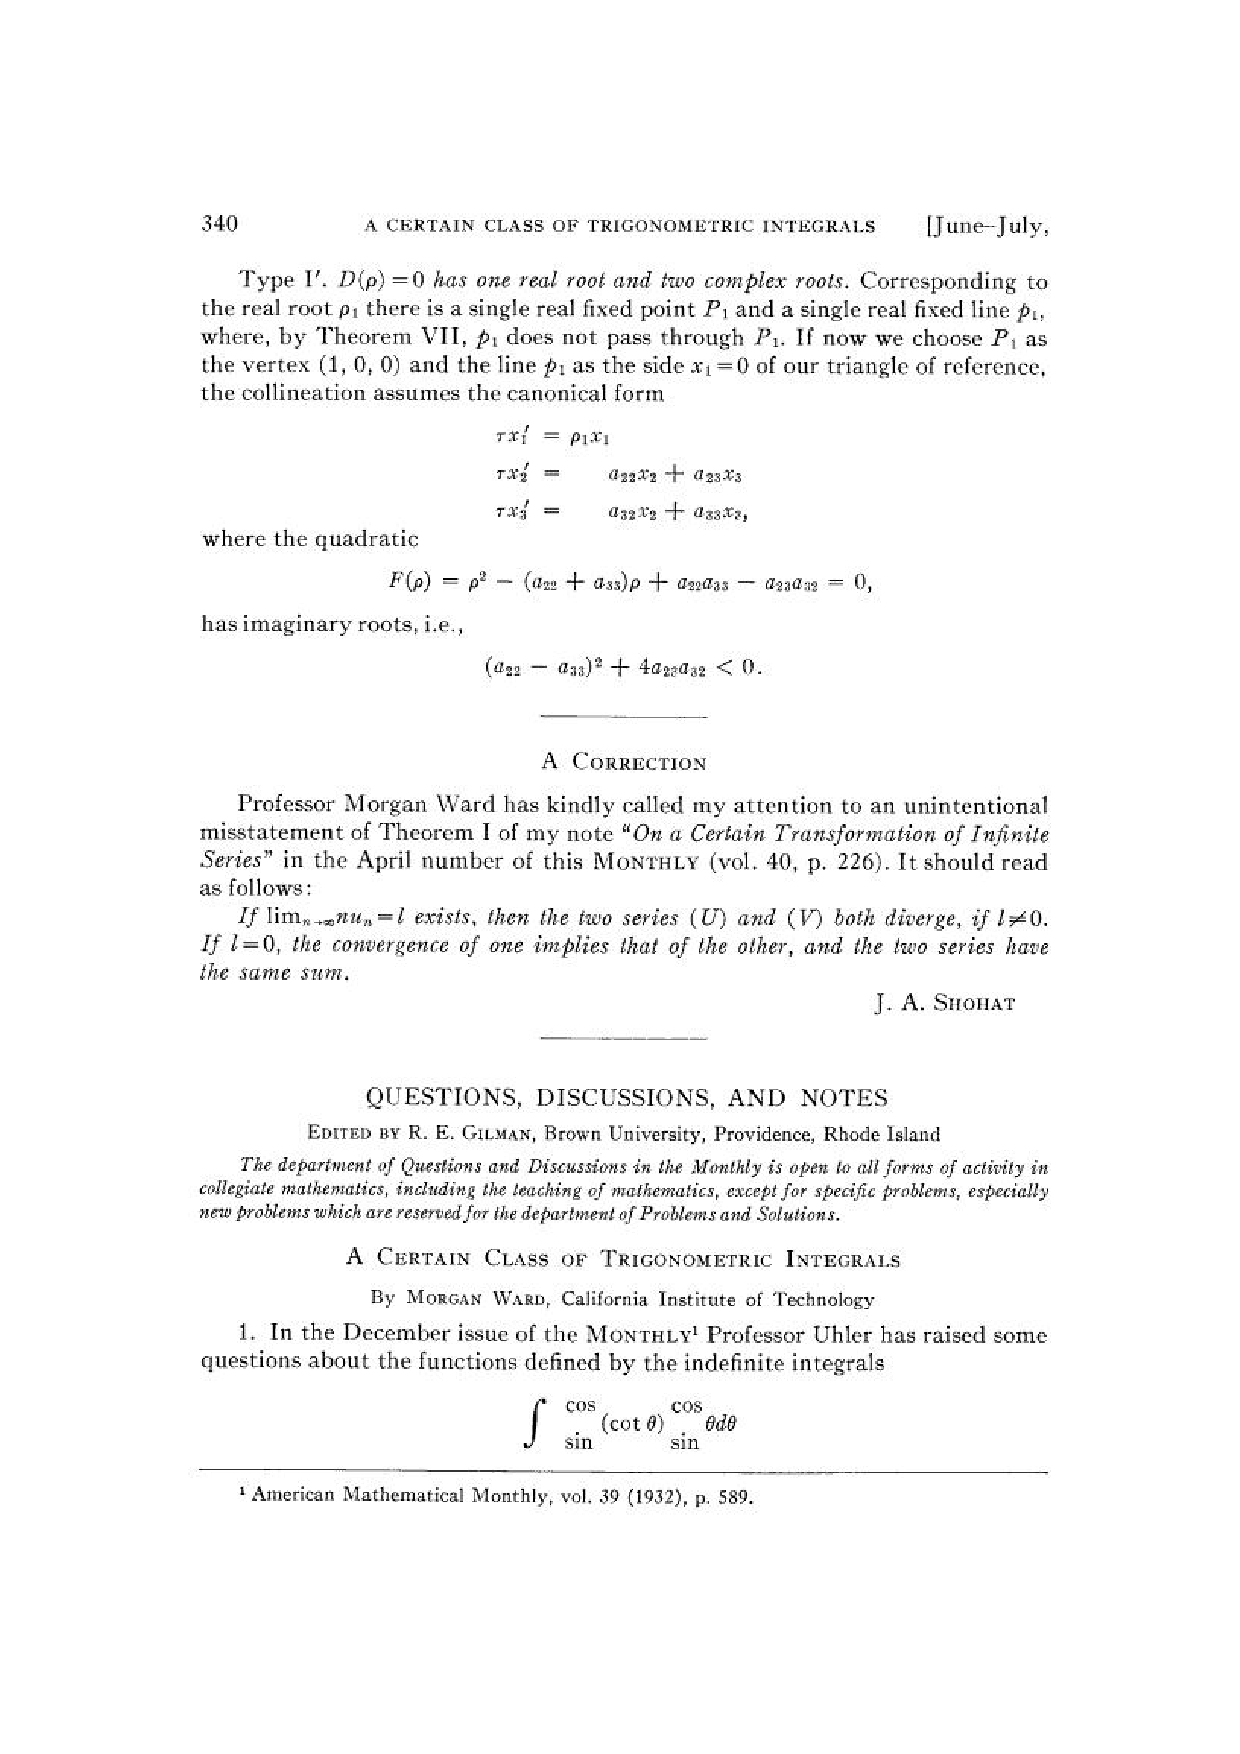
\includepdf[pages={-}]{1933-05 A Certain Class of Trigonometric Integrals.pdf}
	\chapter{1934}
	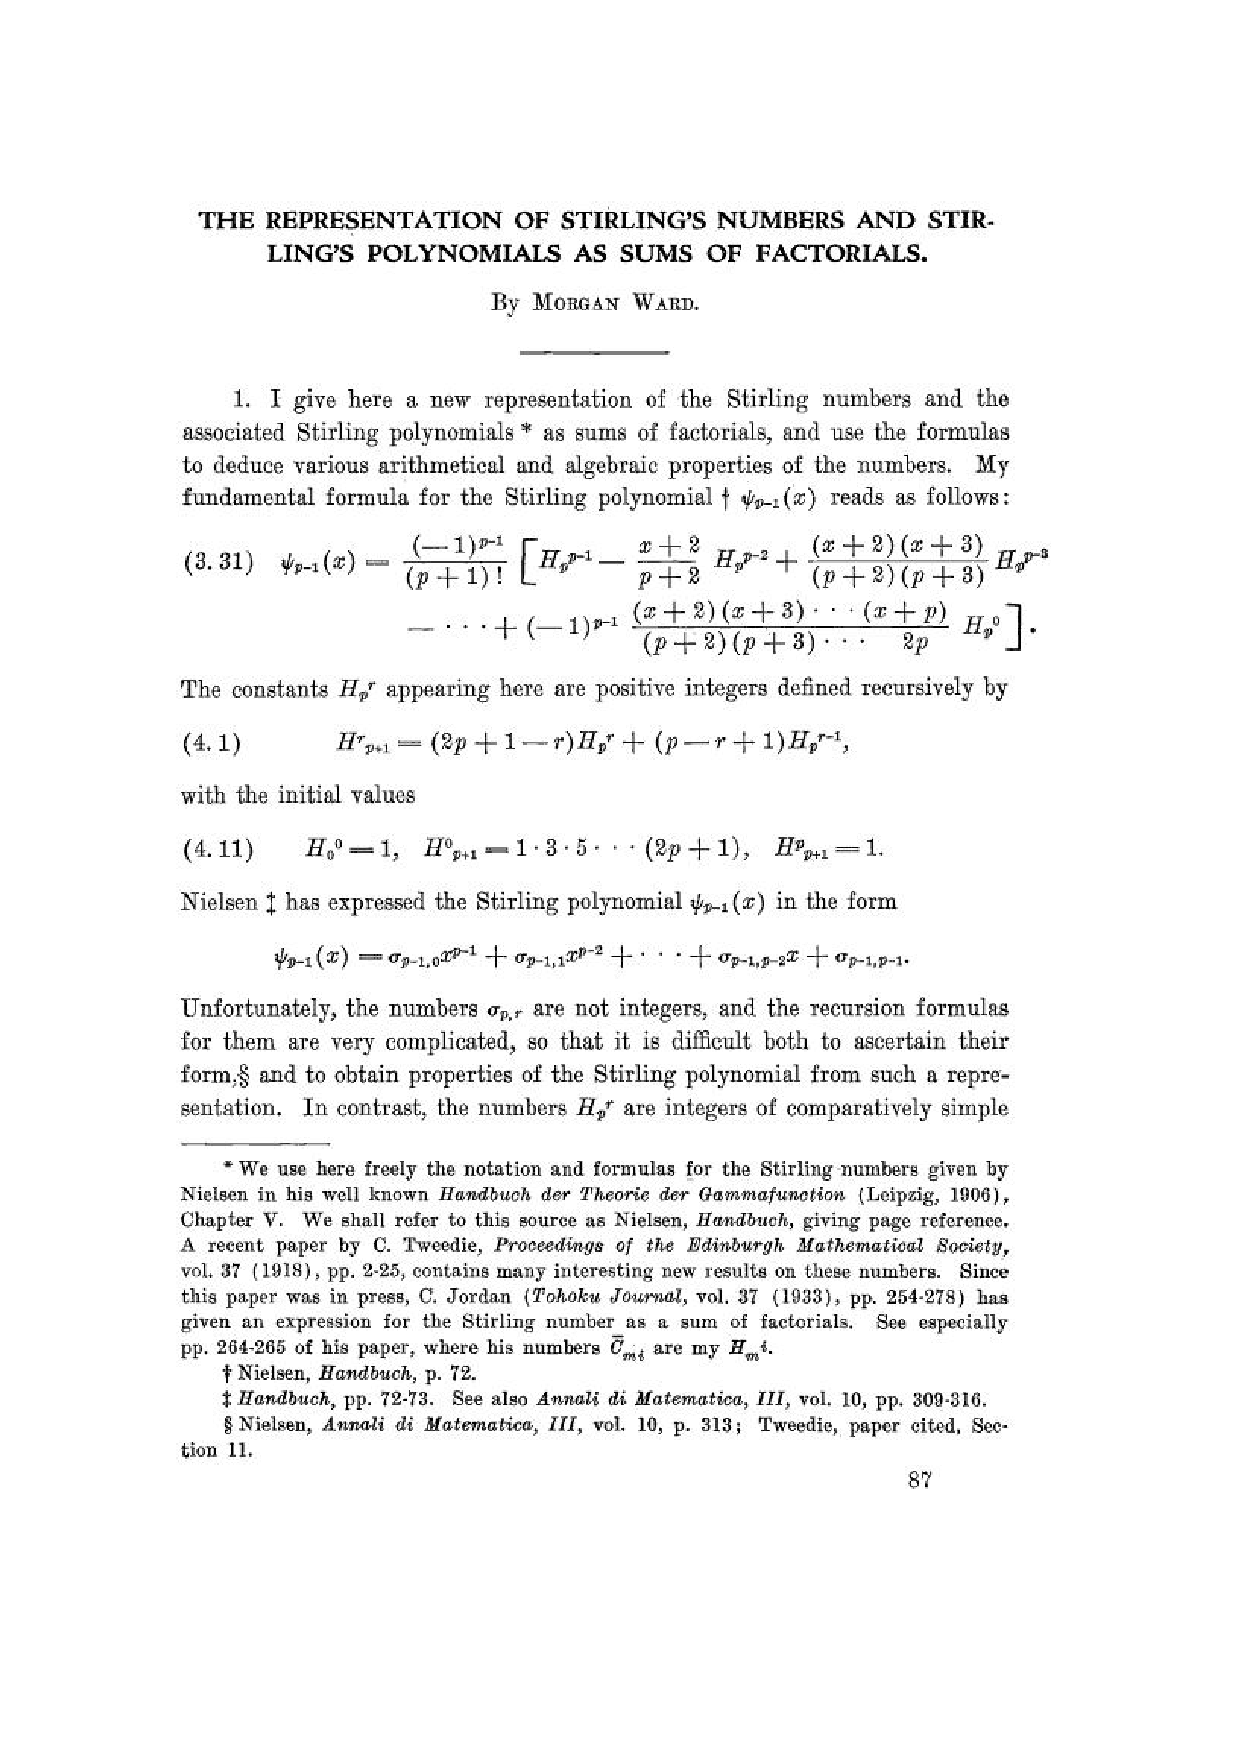
\includepdf[pages={-}]{1934-01 The Representation of Stirling's Numbers and Stirling's Polynomials as Sums of Factorials.pdf}
	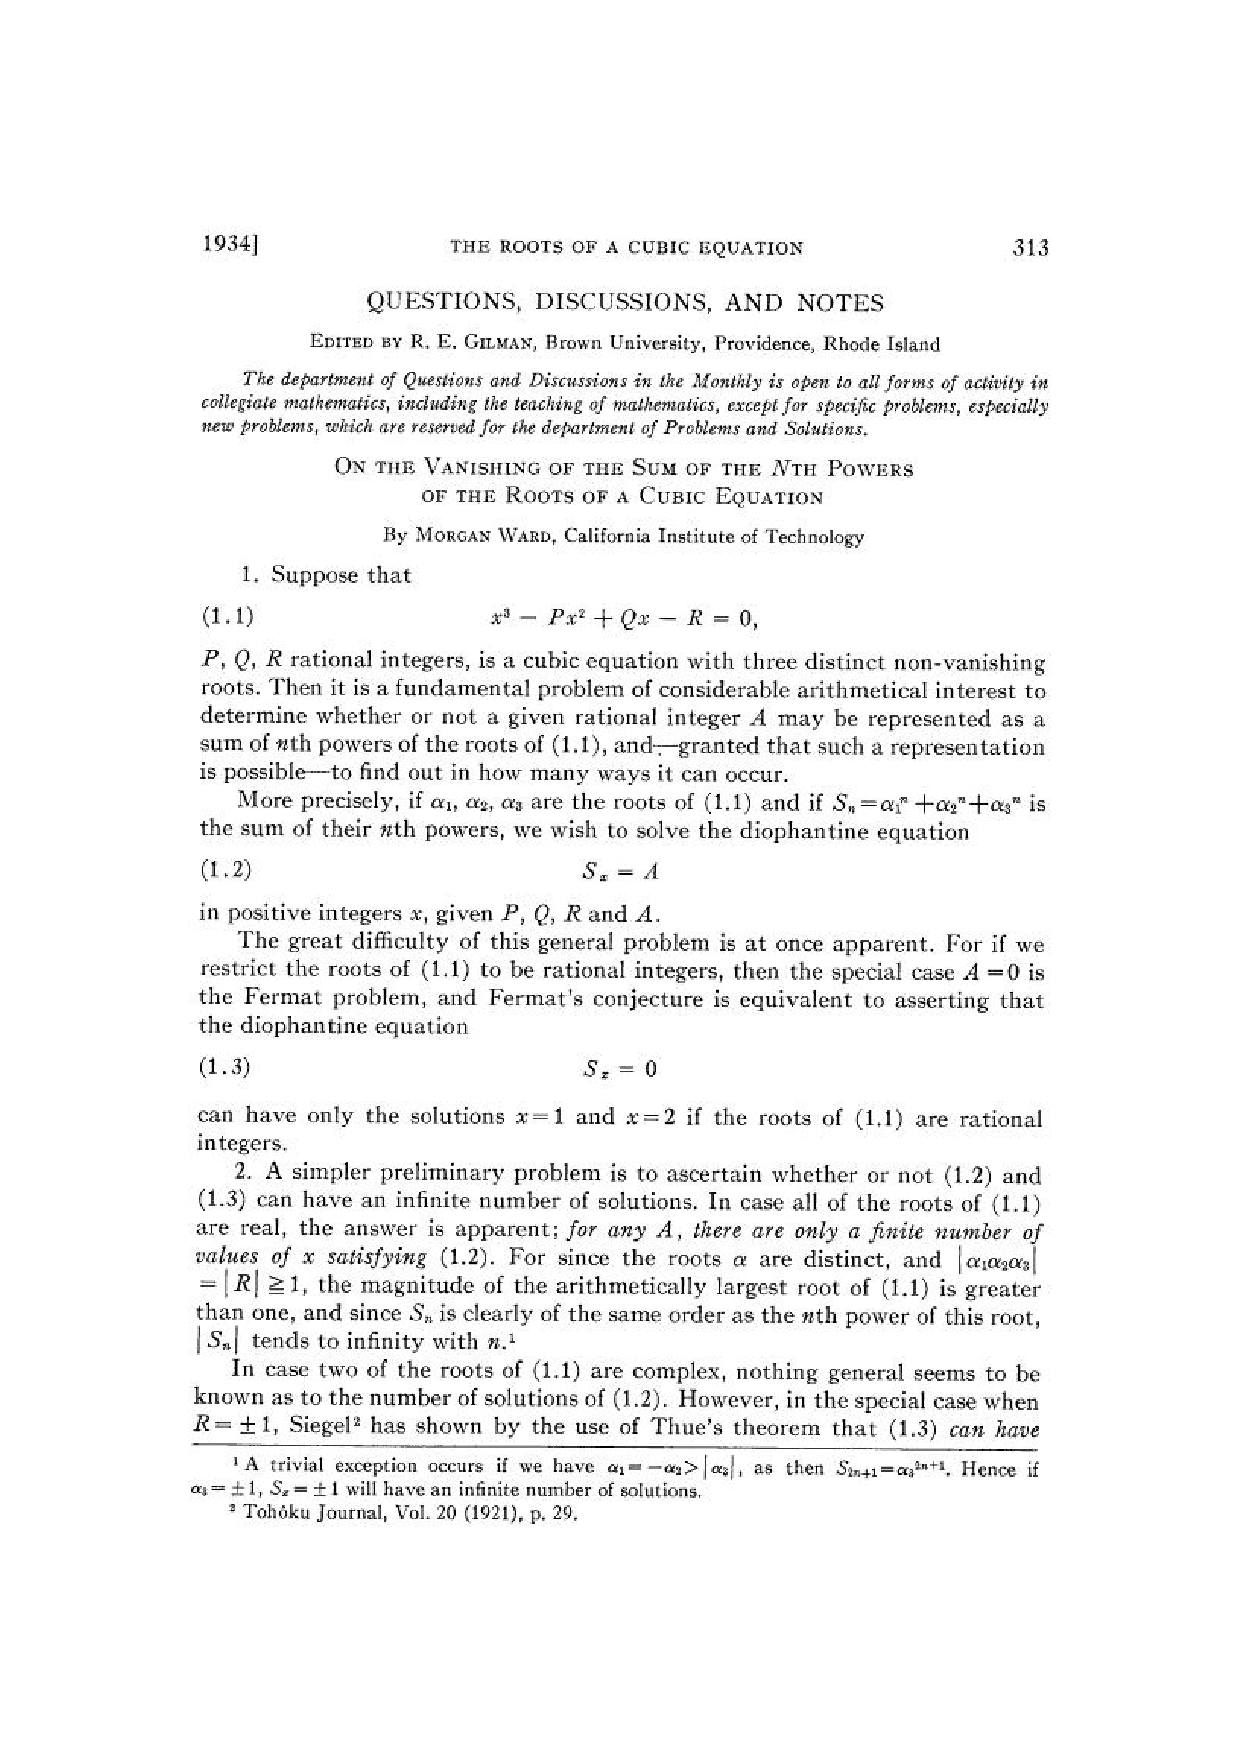
\includepdf[pages={-}]{1934-02 On the Vanishing of the Sum of the Nth Powers of the Roots of a Cubic Equation.pdf}
	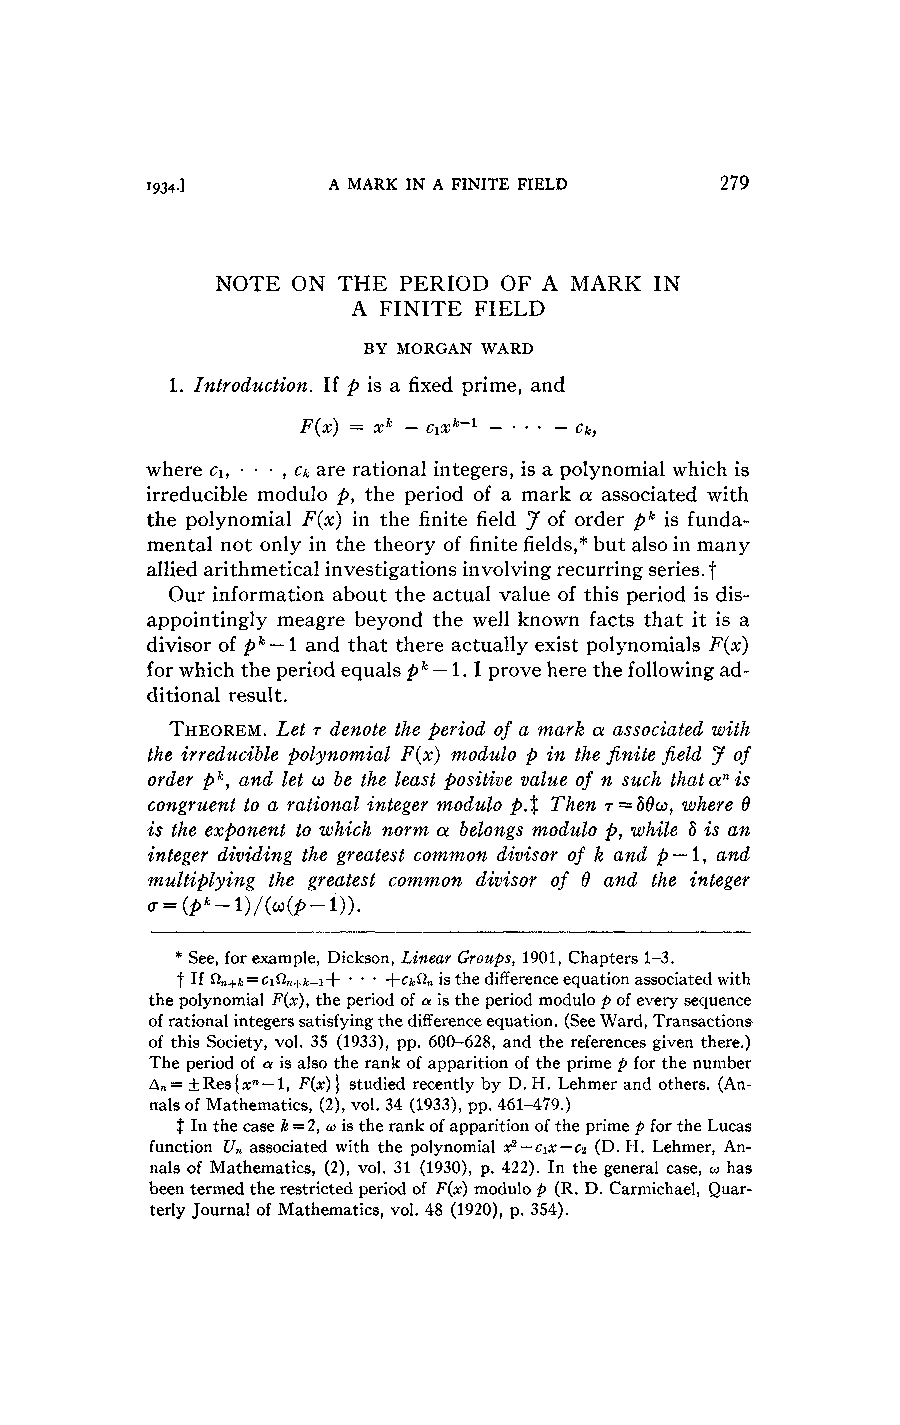
\includepdf[pages={-}]{1934-03 Note on the period of a mark in a finite field.pdf}
	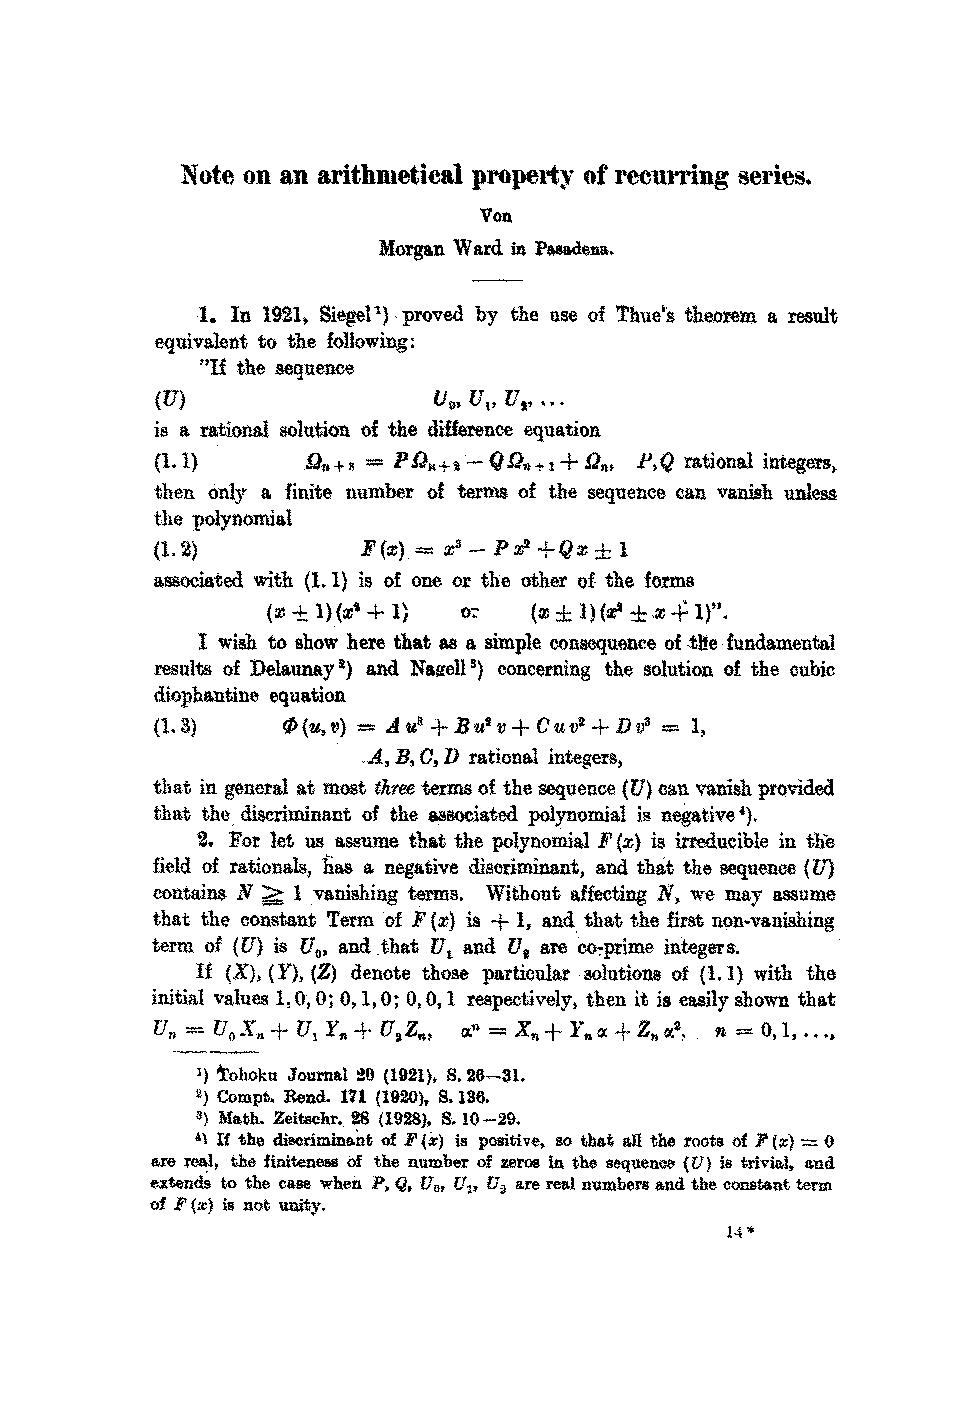
\includepdf[pages={-}]{1934-04 Note on an arithmetical property of recurring series.pdf}
	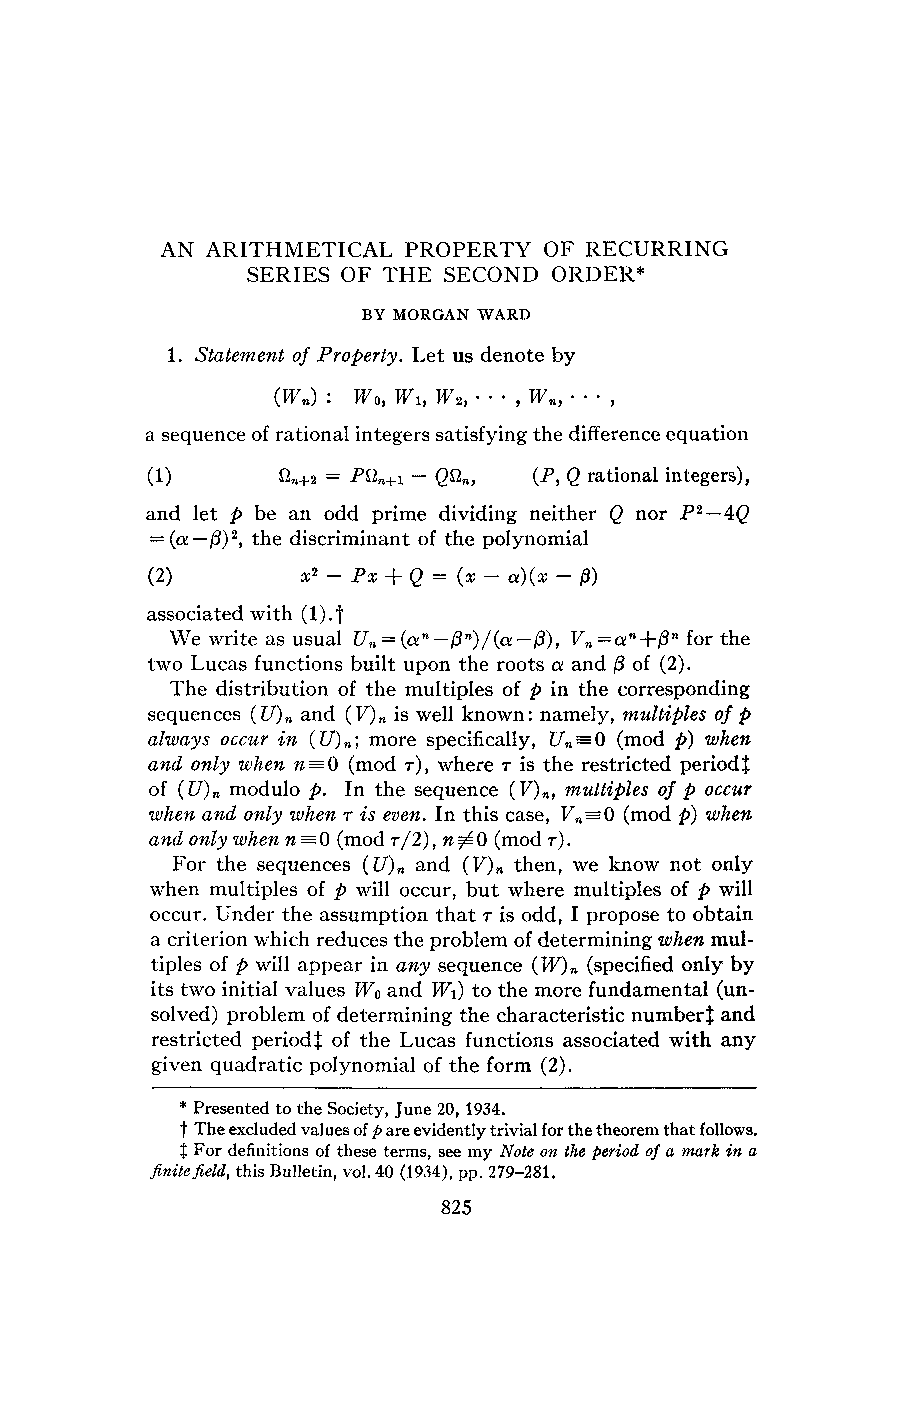
\includepdf[pages={-}]{1934-05 An arithmetical property of recurring series of the second order.pdf}
	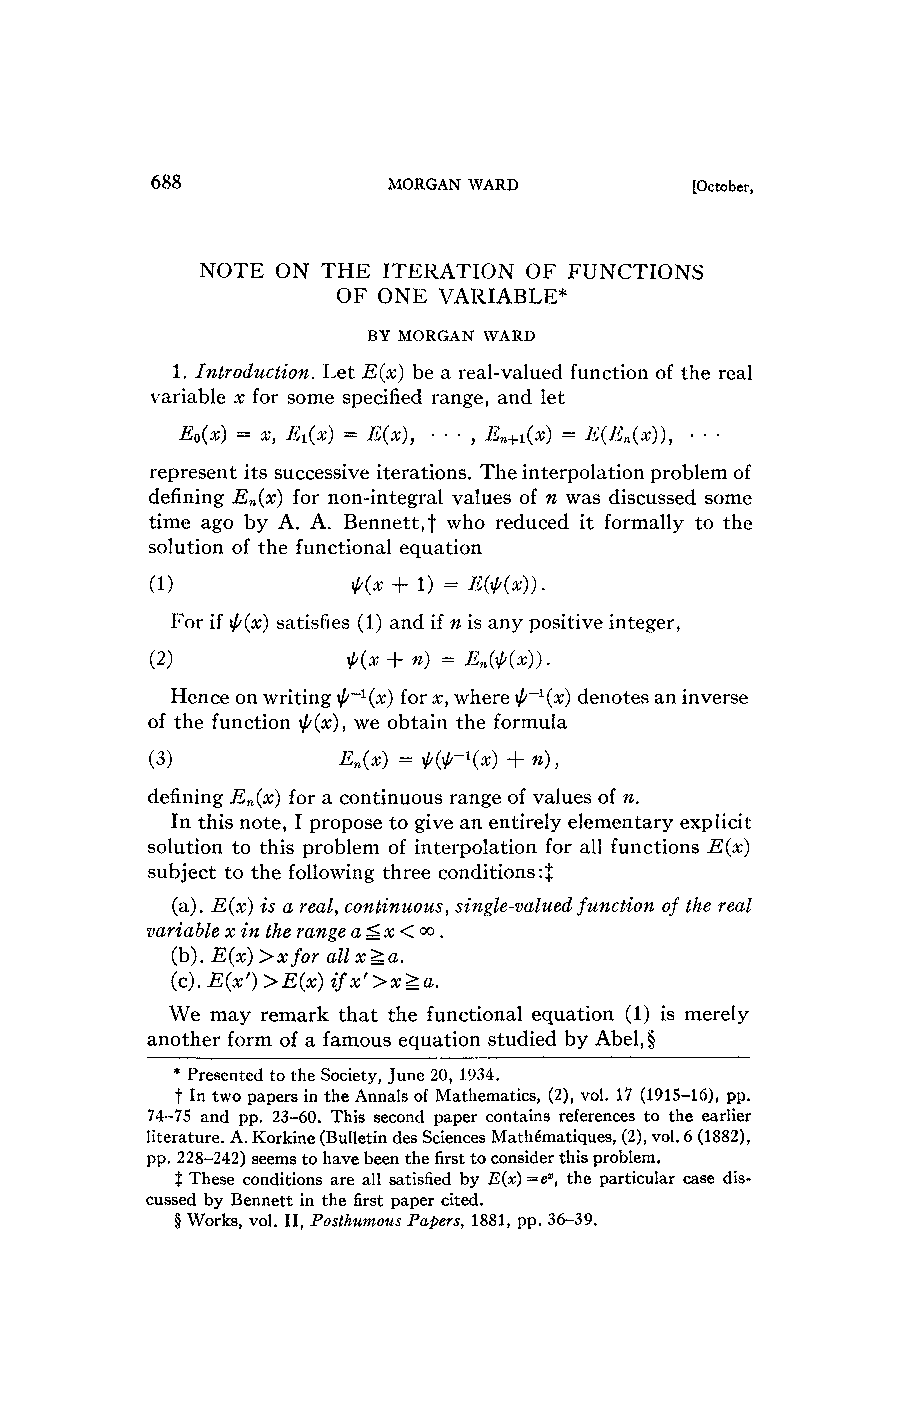
\includepdf[pages={-}]{1934-06 Note on the iteration of functions of one variable.pdf}
	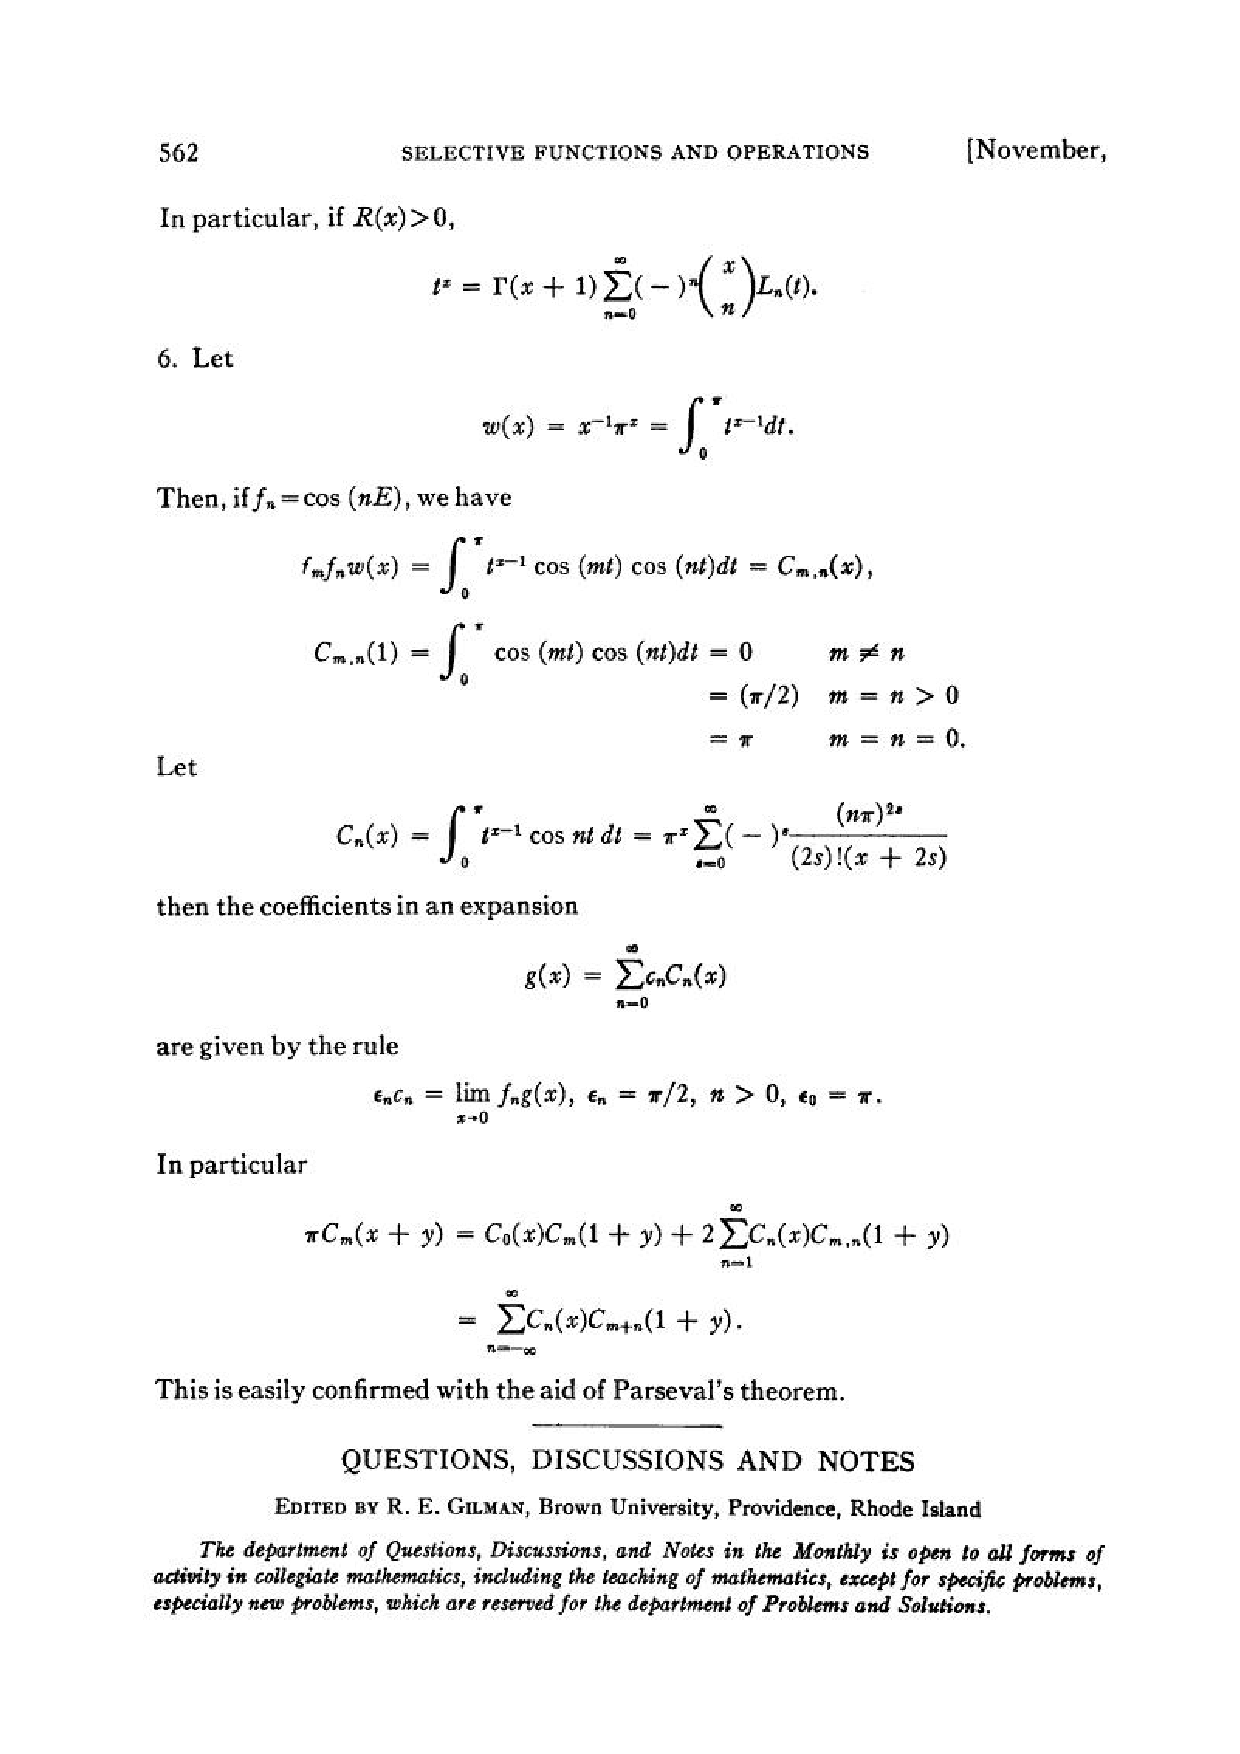
\includepdf[pages={-}]{1934-07 The Numerical Evaluation of a Class of Trigonometric Series.pdf}
	\chapter{1935}
	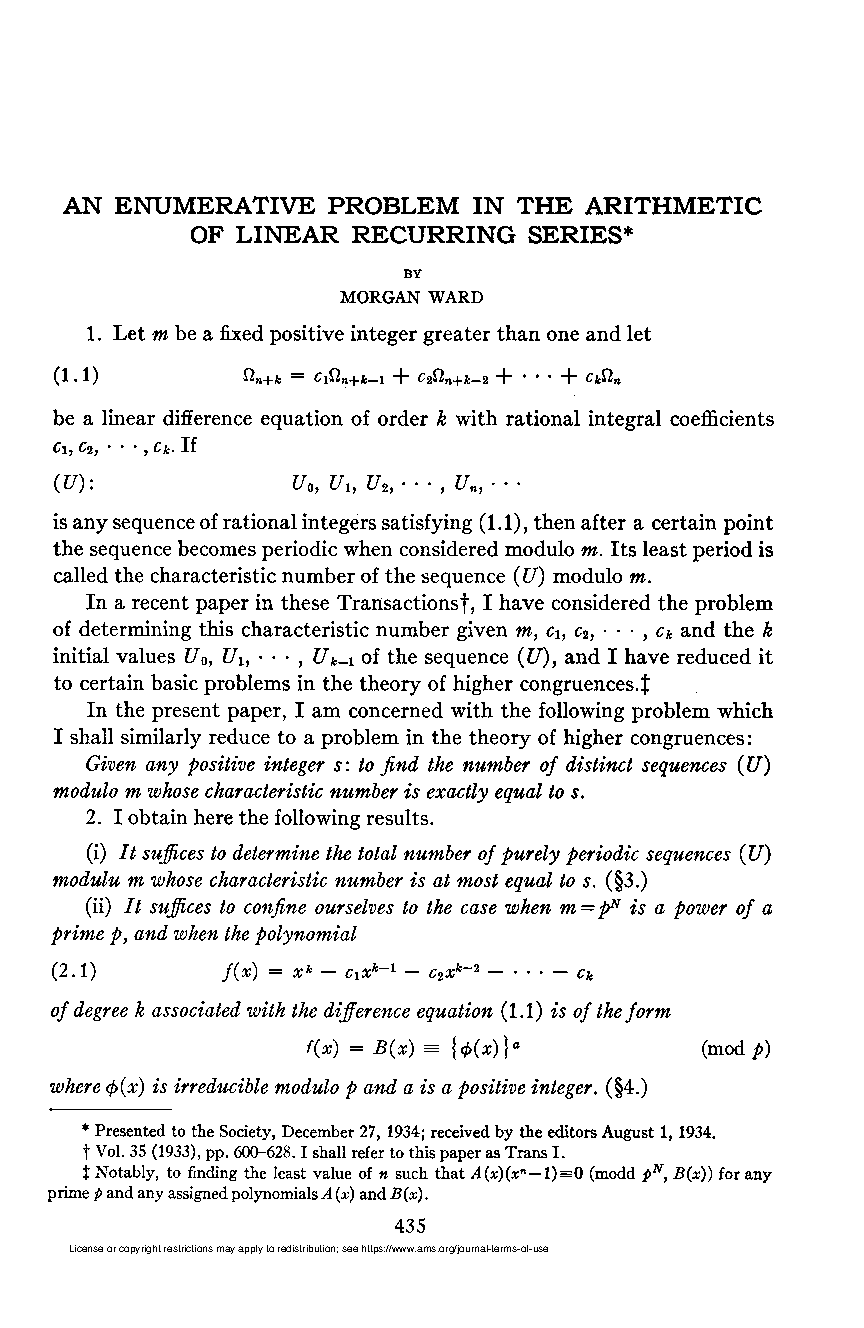
\includepdf[pages={-}]{1935-01 An enumerative problem in the arithmetic of linear recurring series.pdf}
	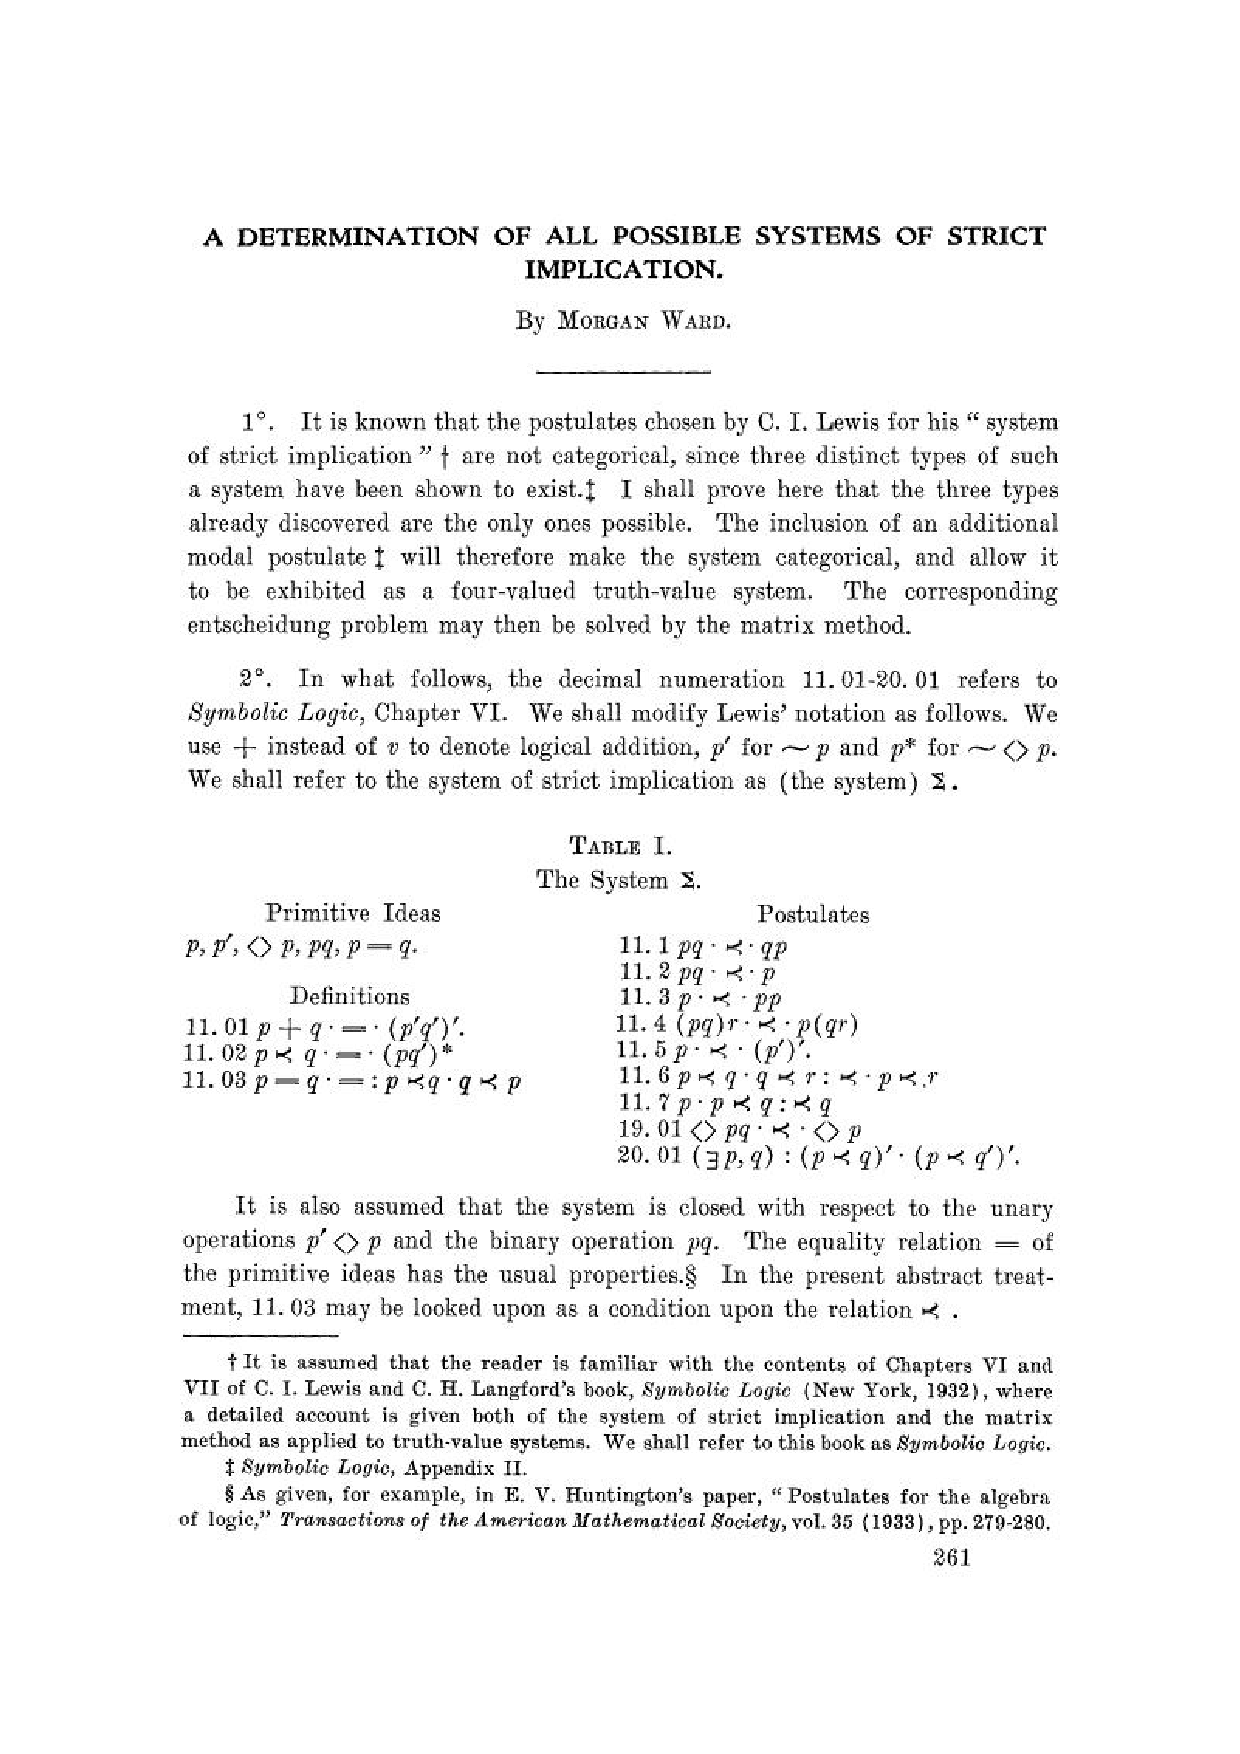
\includepdf[pages={-}]{1935-02 A Determination of all Possible Systems of Strict Implication.pdf}
	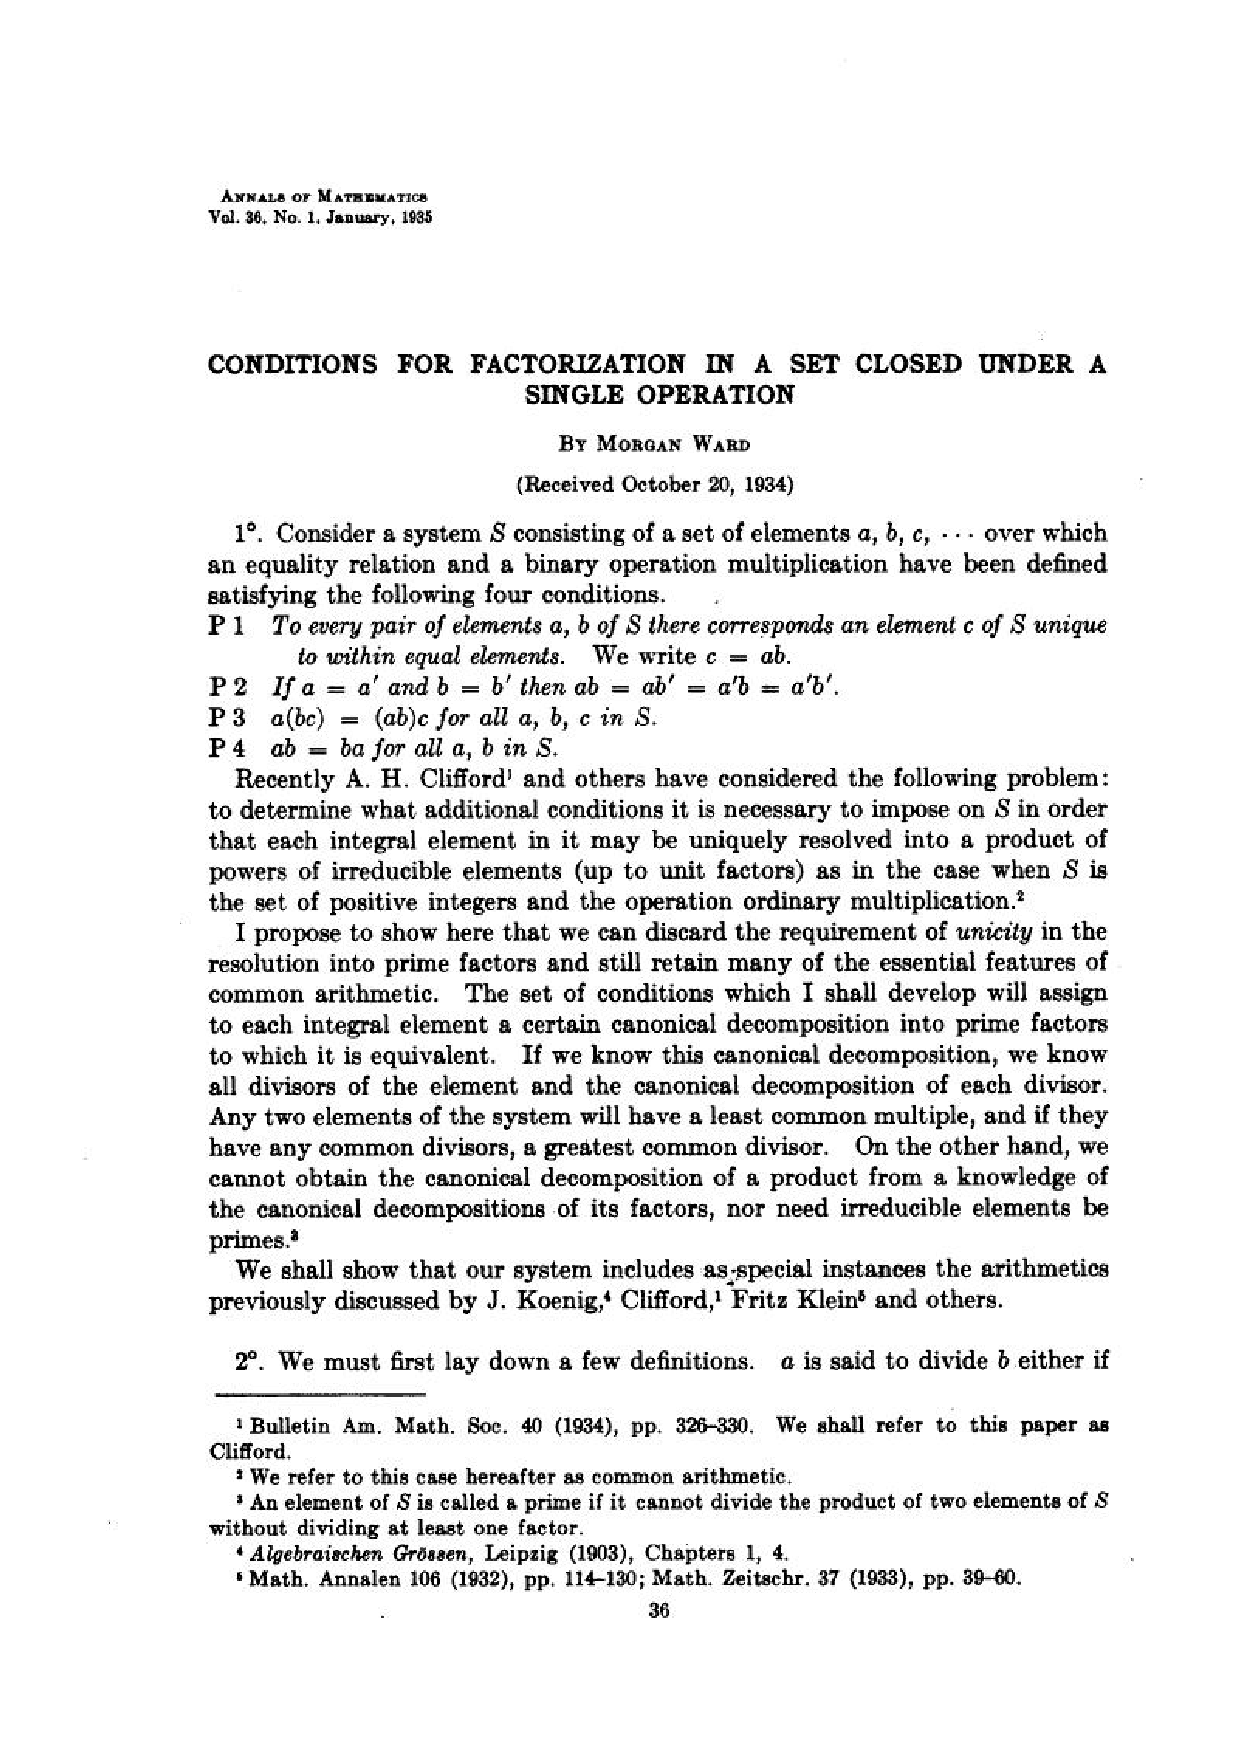
\includepdf[pages={-}]{1935-03 Conditions for Factorization in a Set Closed Under a Single Operation.pdf}
	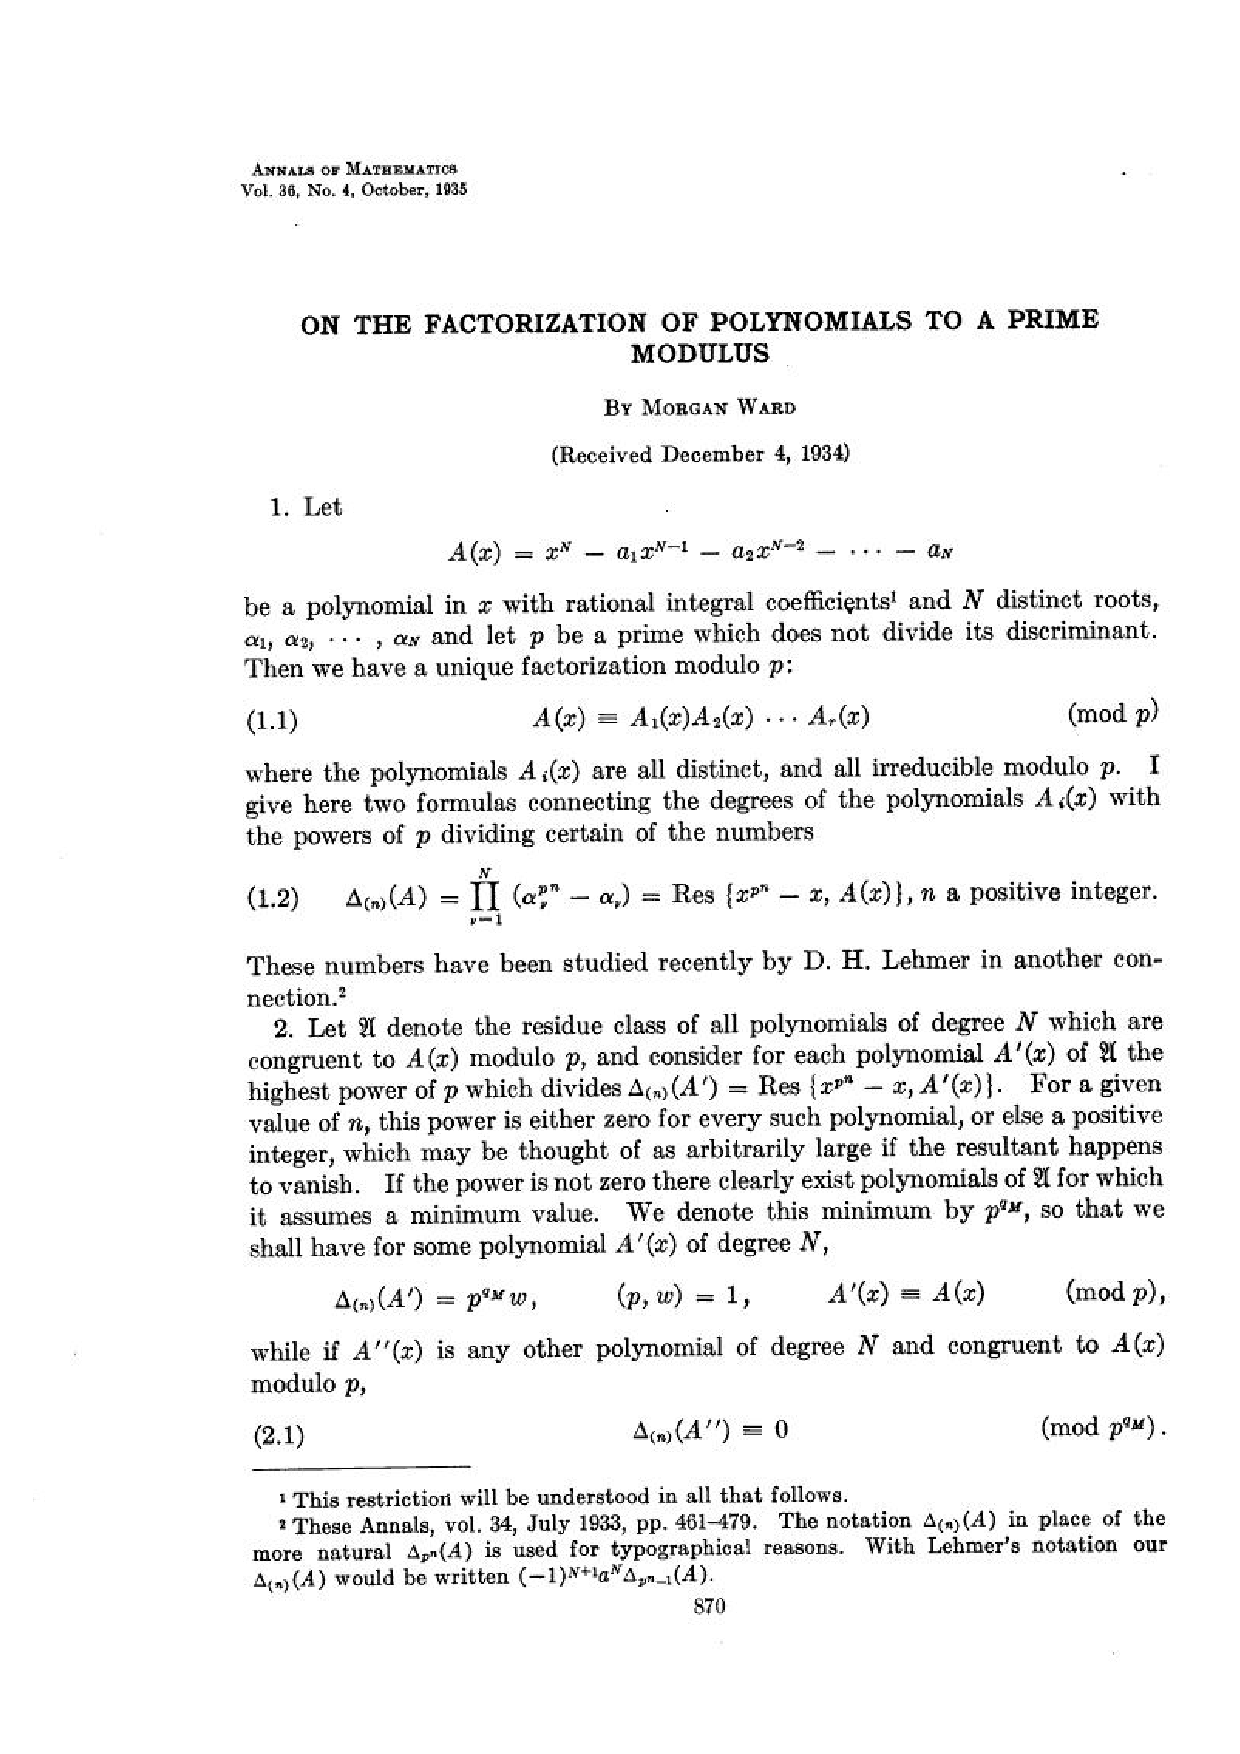
\includepdf[pages={-}]{1935-04 On the Factorization of Polynomials to a Prime Modulus.pdf}
	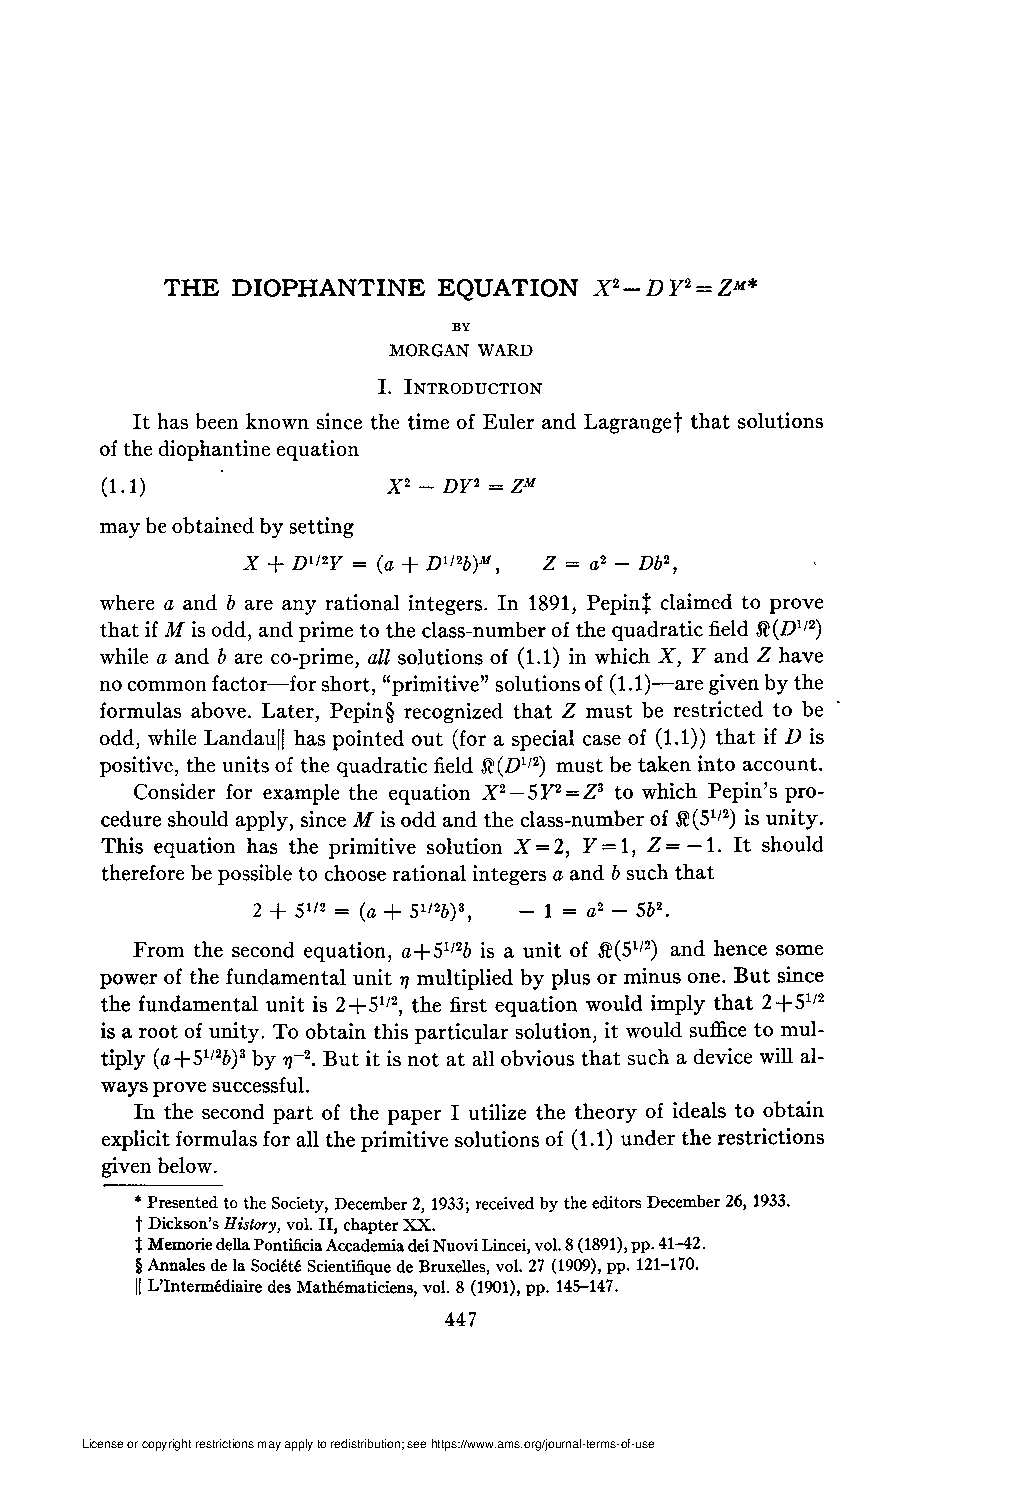
\includepdf[pages={-}]{1935-05 The diophantine equation.pdf}
	\chapter{1936}
	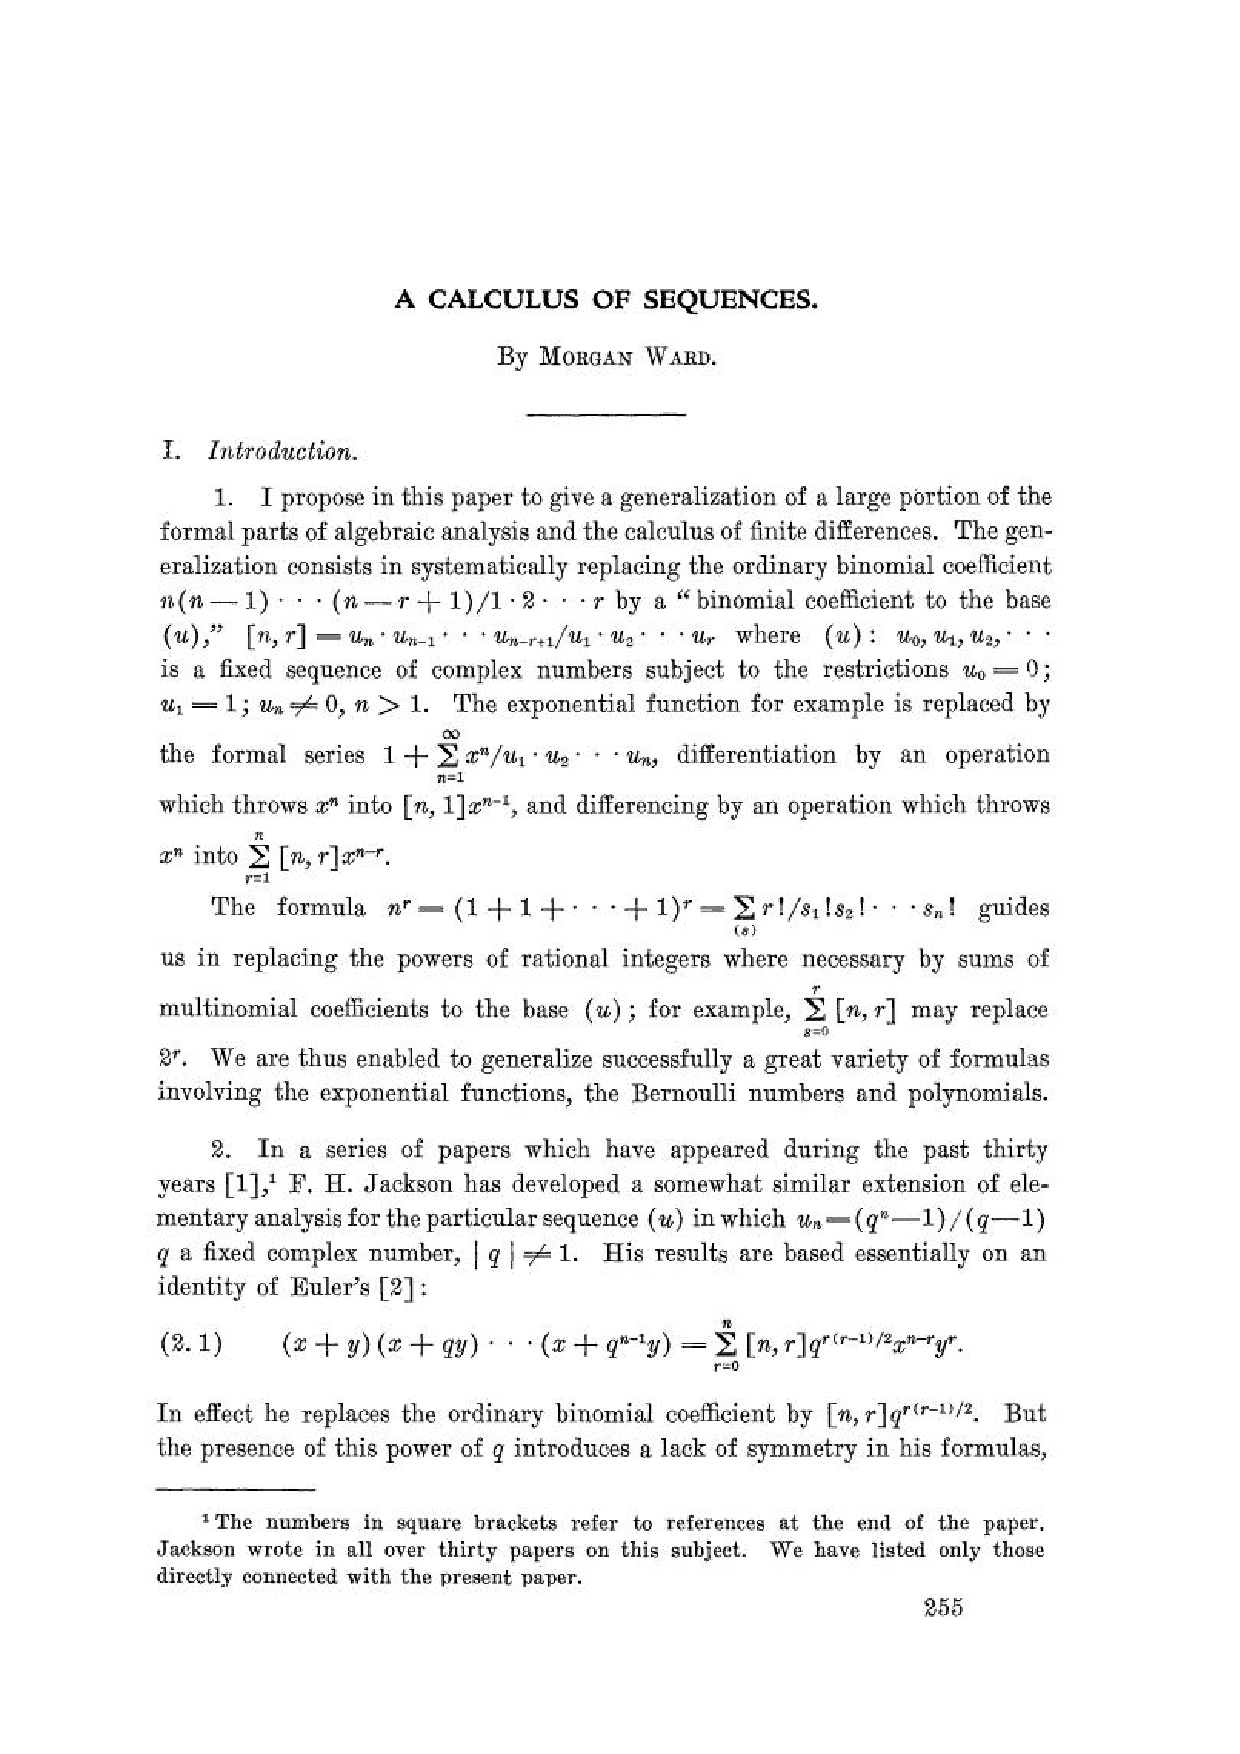
\includepdf[pages={-}]{1936-01 A Calculus of Sequences.pdf}
	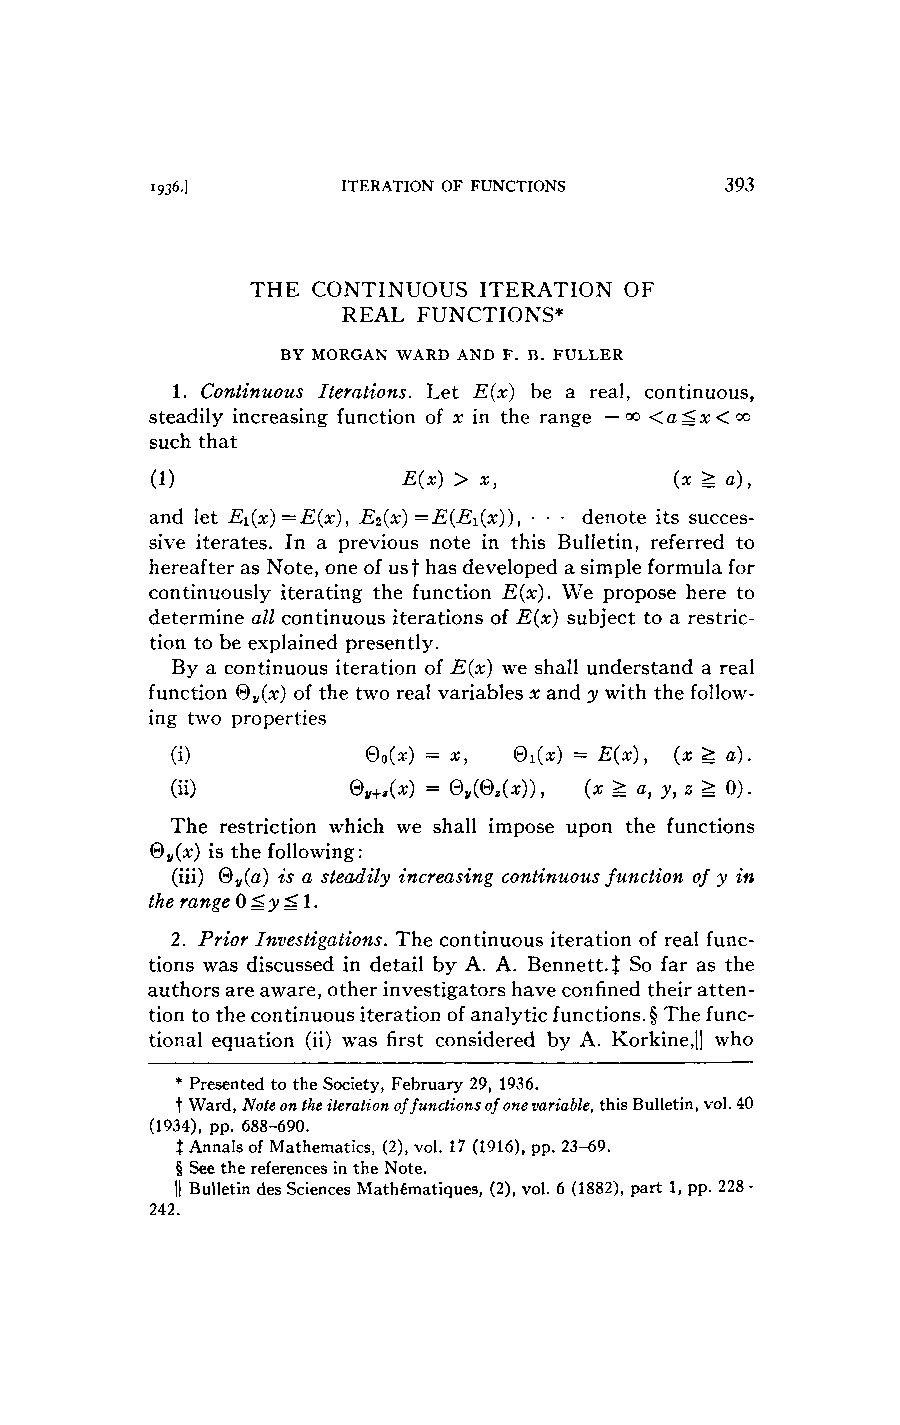
\includepdf[pages={-}]{1936-02 The continuous iteration of real functions.pdf}
	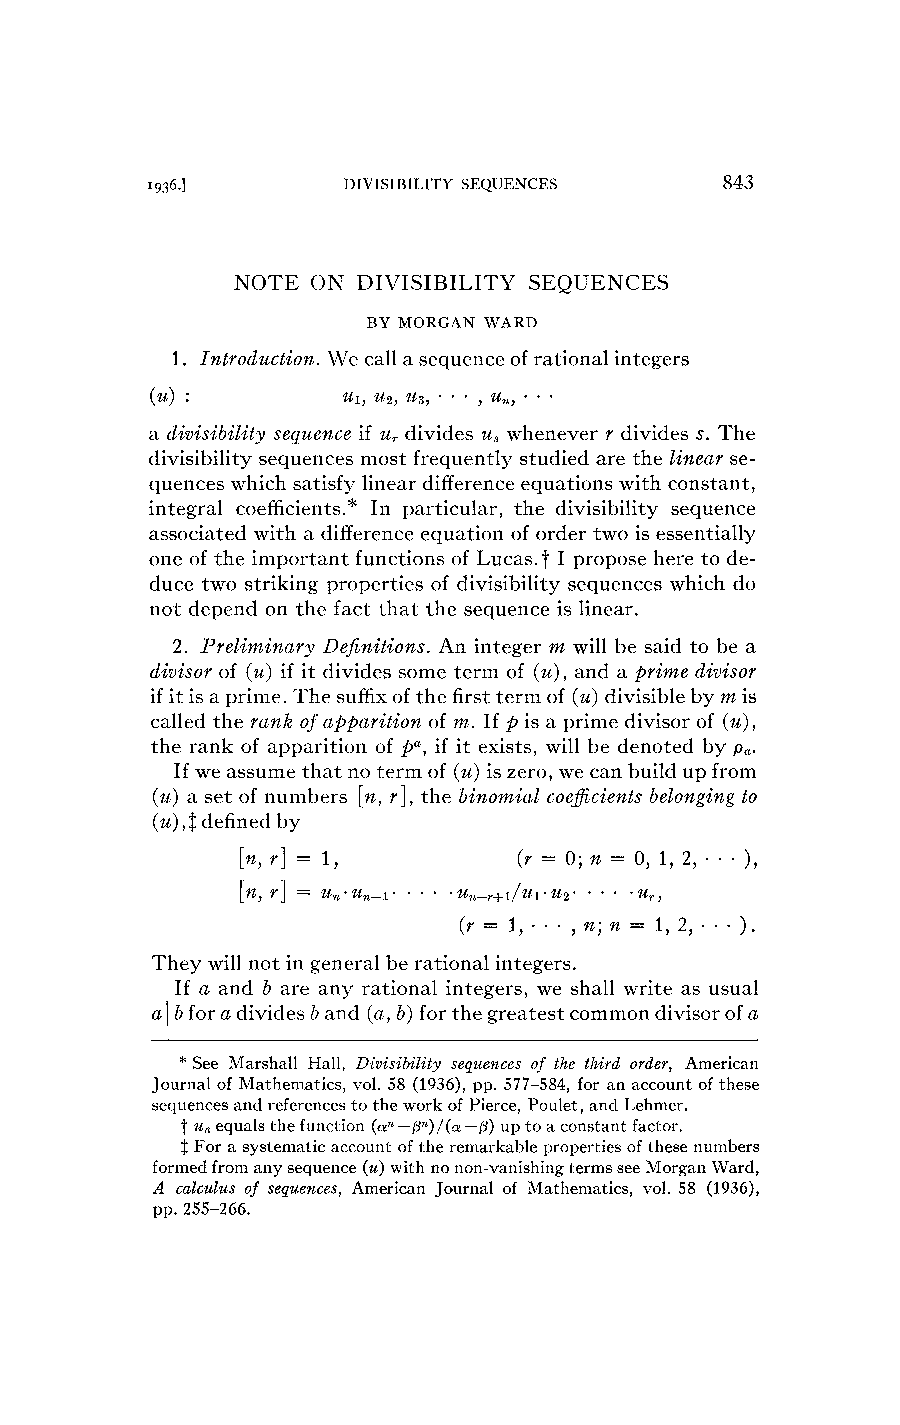
\includepdf[pages={-}]{1936-04 Note on divisibility sequences.pdf}
	\chapter{1937}
	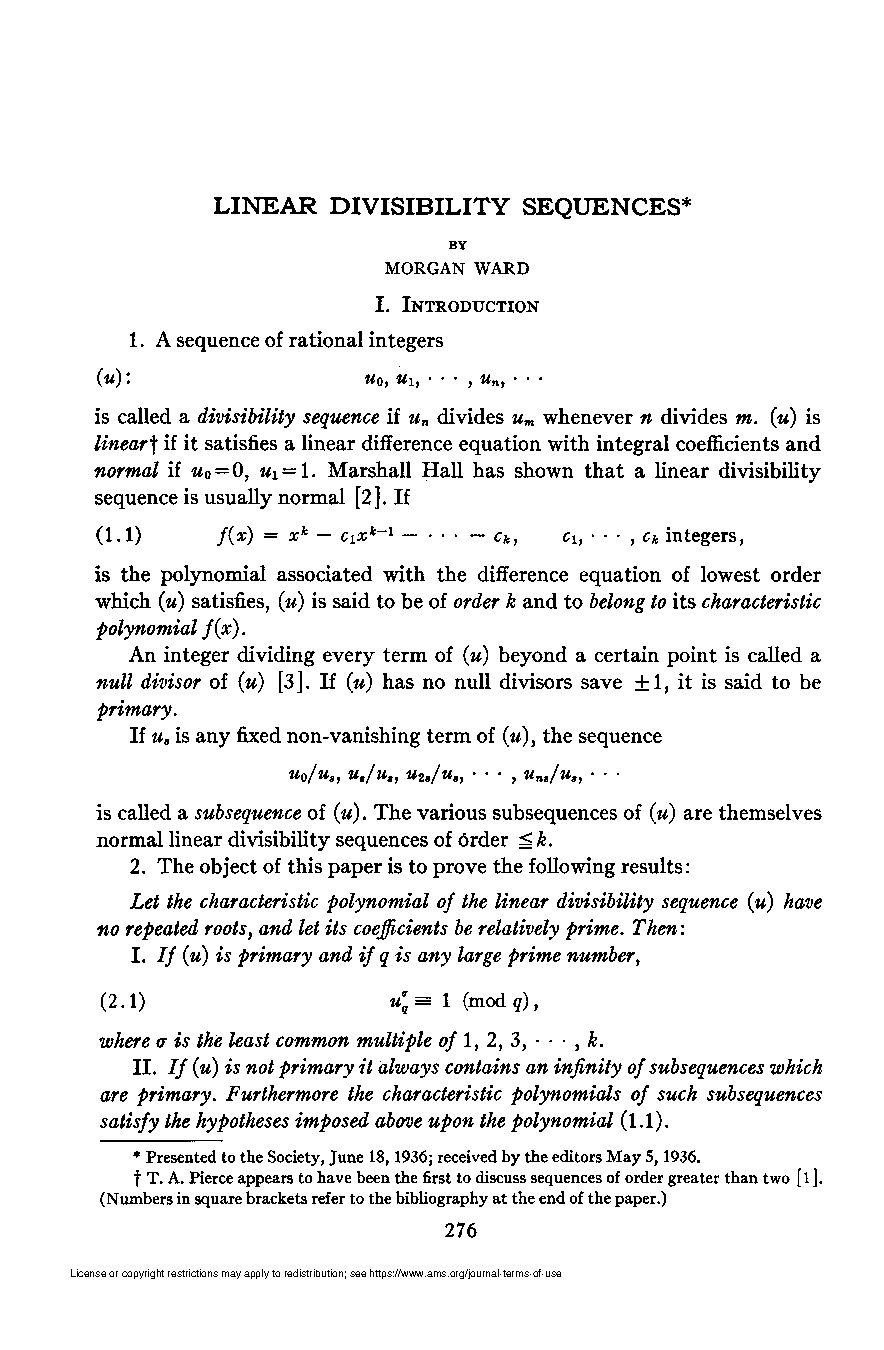
\includepdf[pages={-}]{1937-01 Linear divisibility sequences.pdf}
	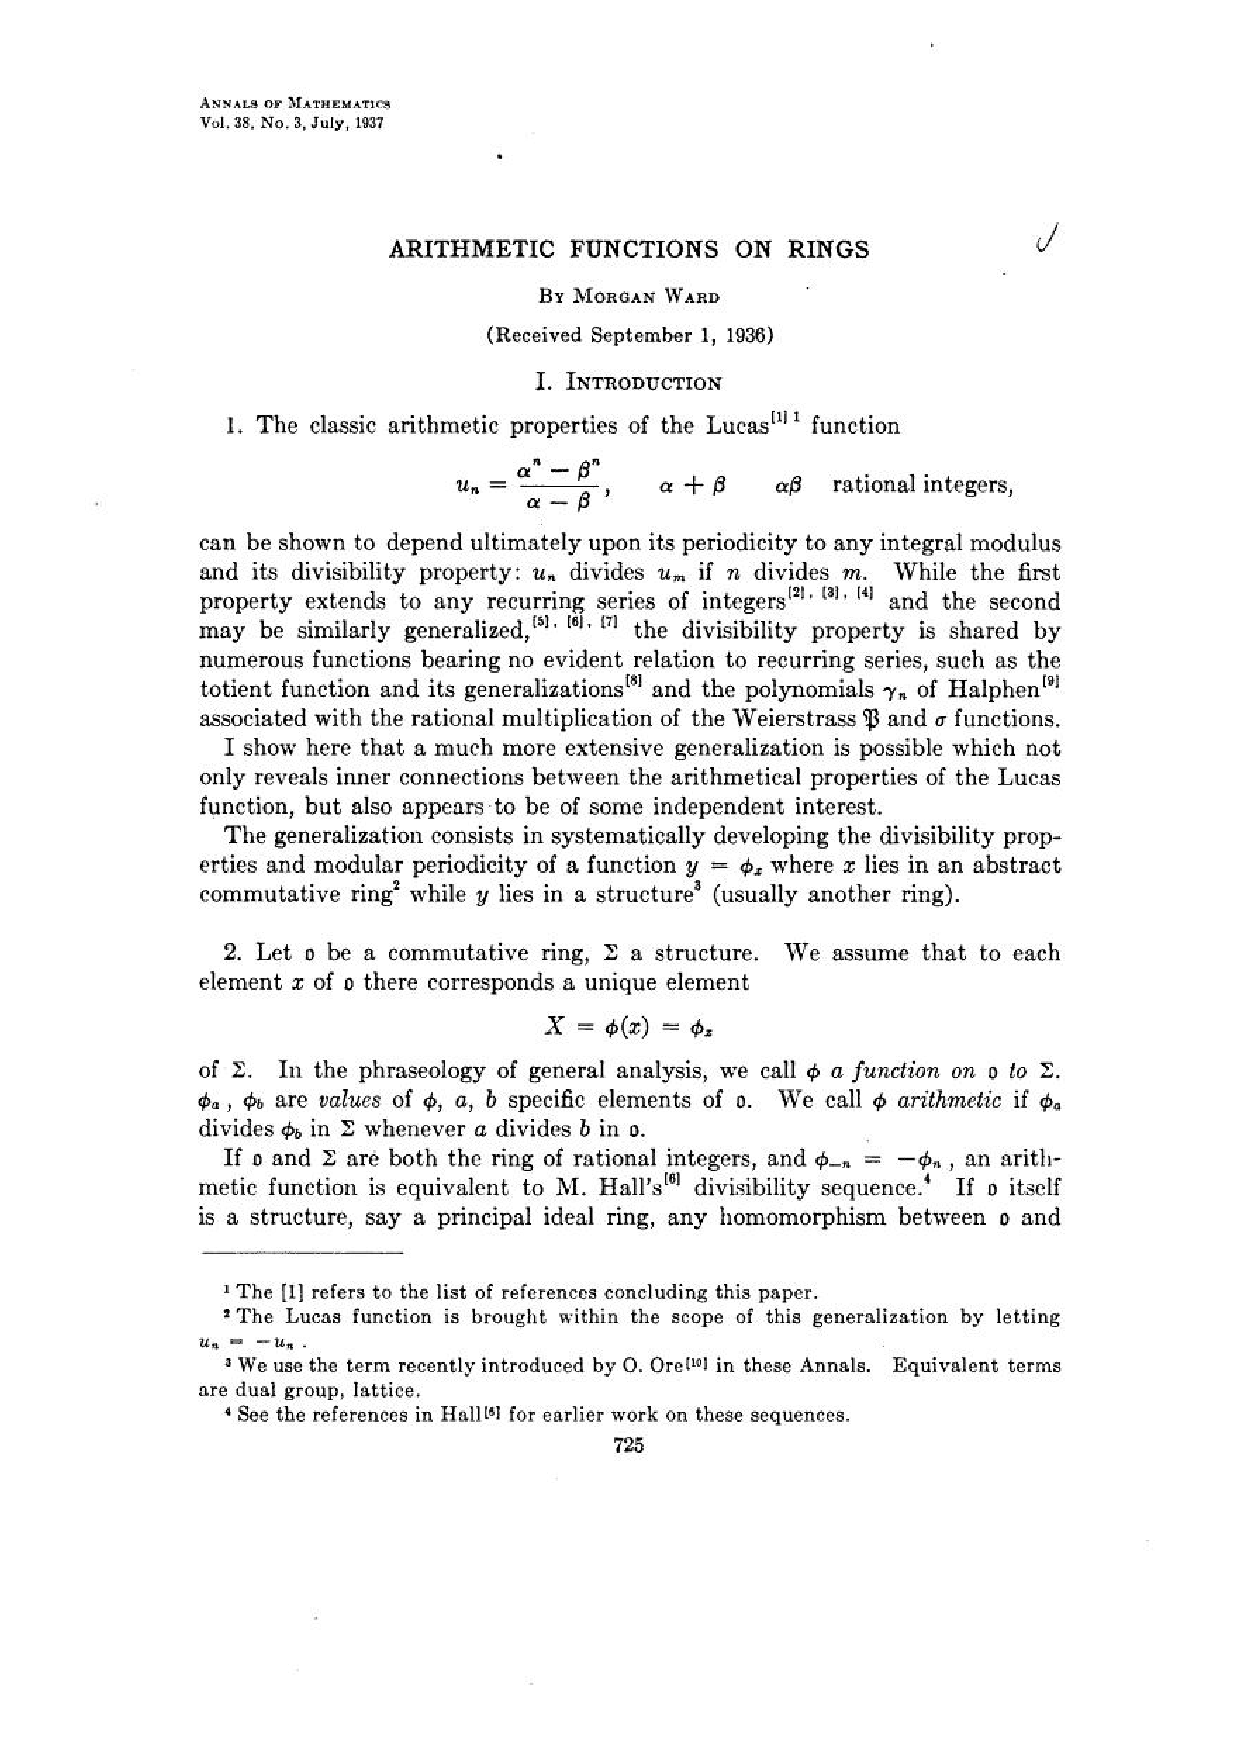
\includepdf[pages={-}]{1937-02 Arithmetic Functions on Rings.pdf}
	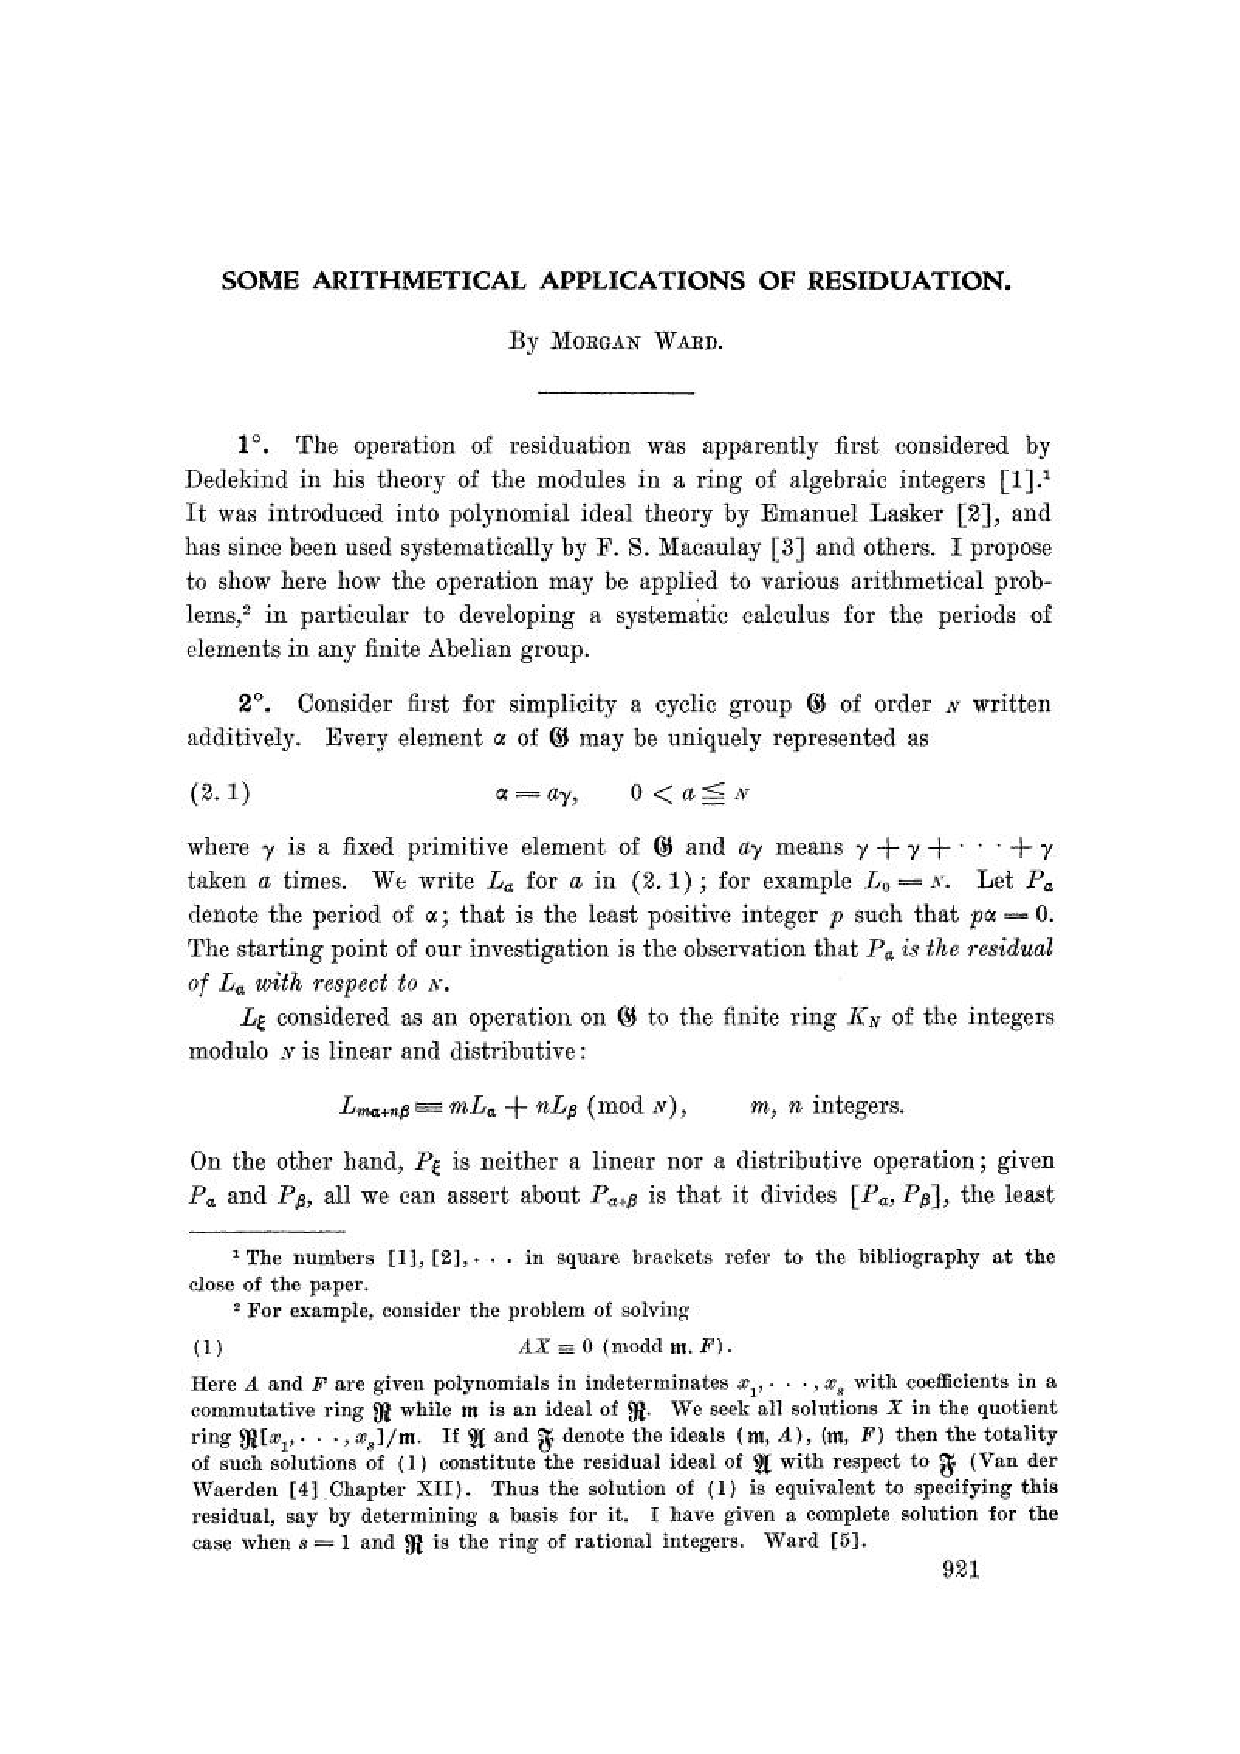
\includepdf[pages={-}]{1937-03 Some Arithmetical Applications of Residuation.pdf}
	\chapter{1938}
	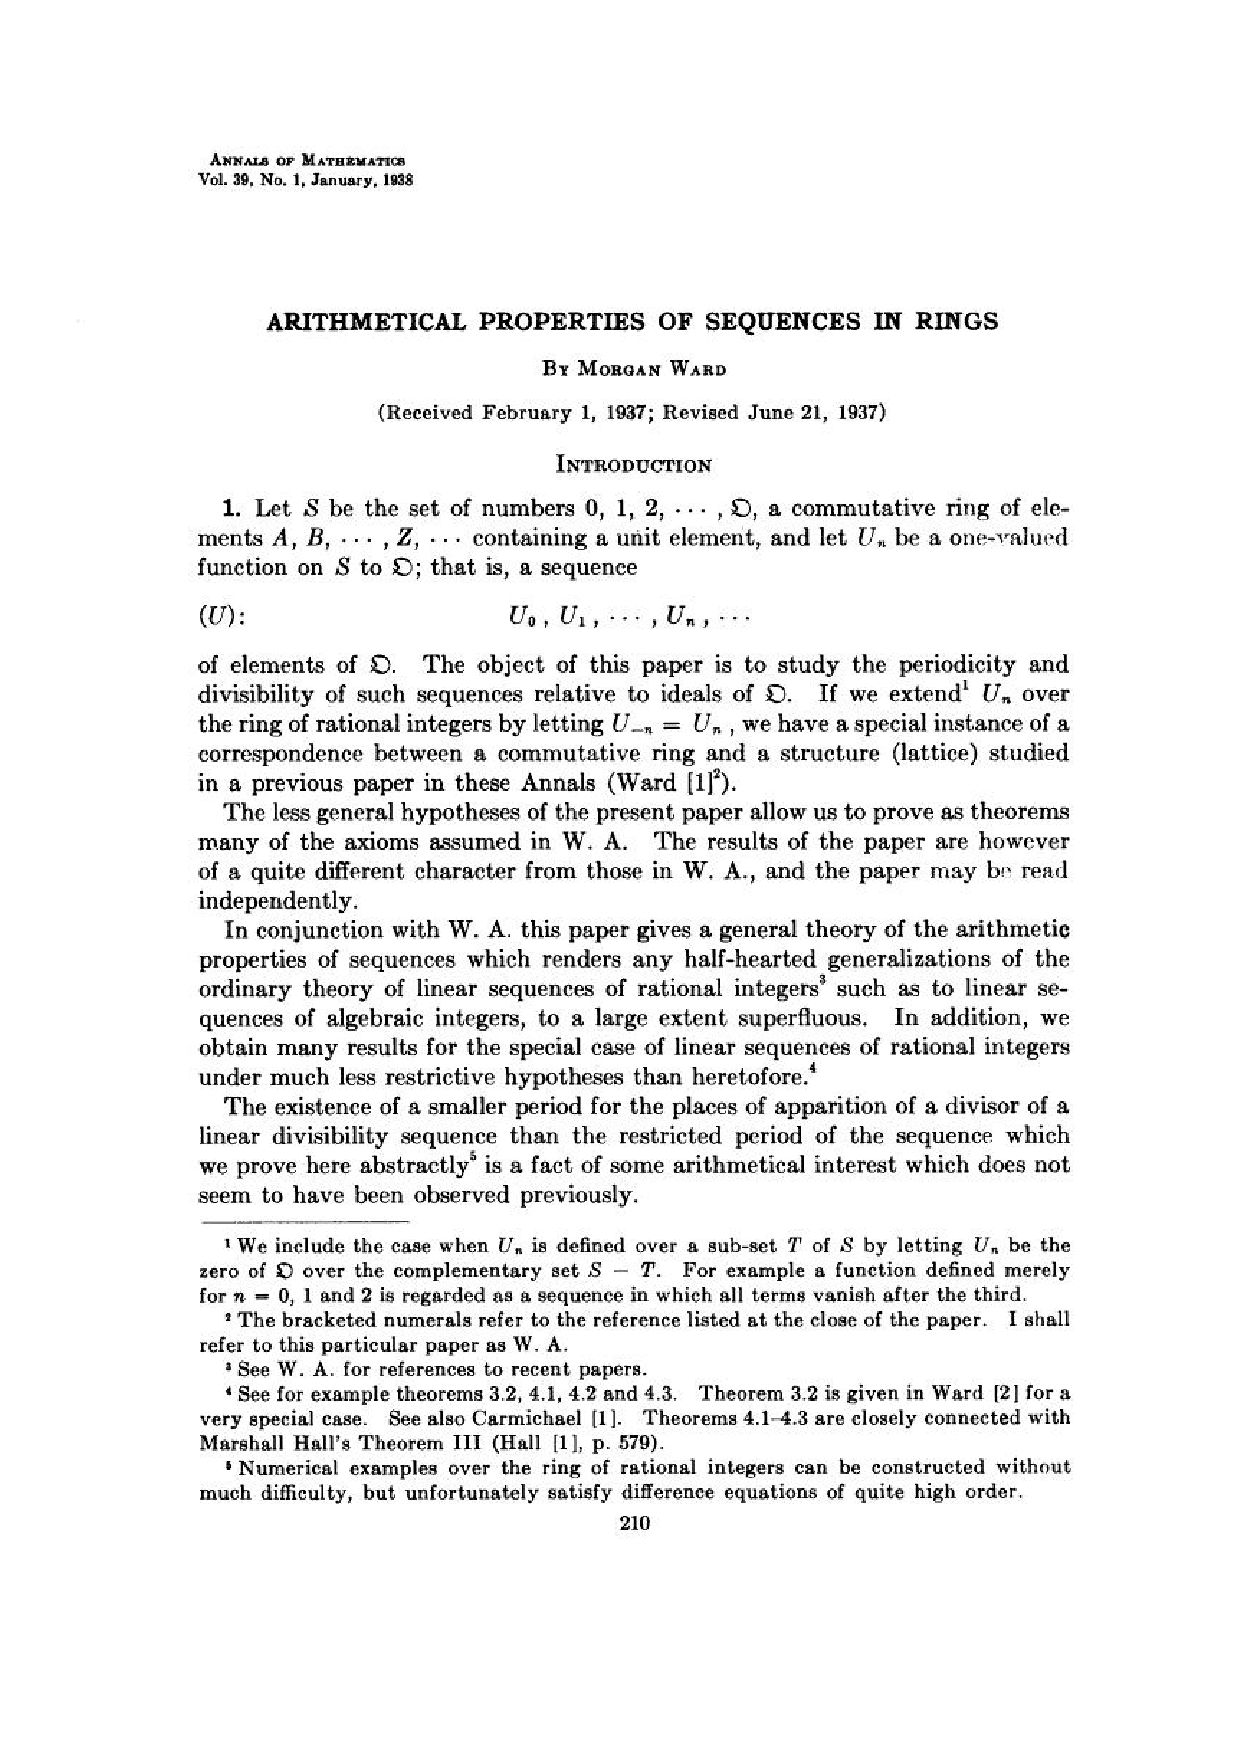
\includepdf[pages={-}]{1938-01 Arithmetical Properties of Sequences in Rings.pdf}
	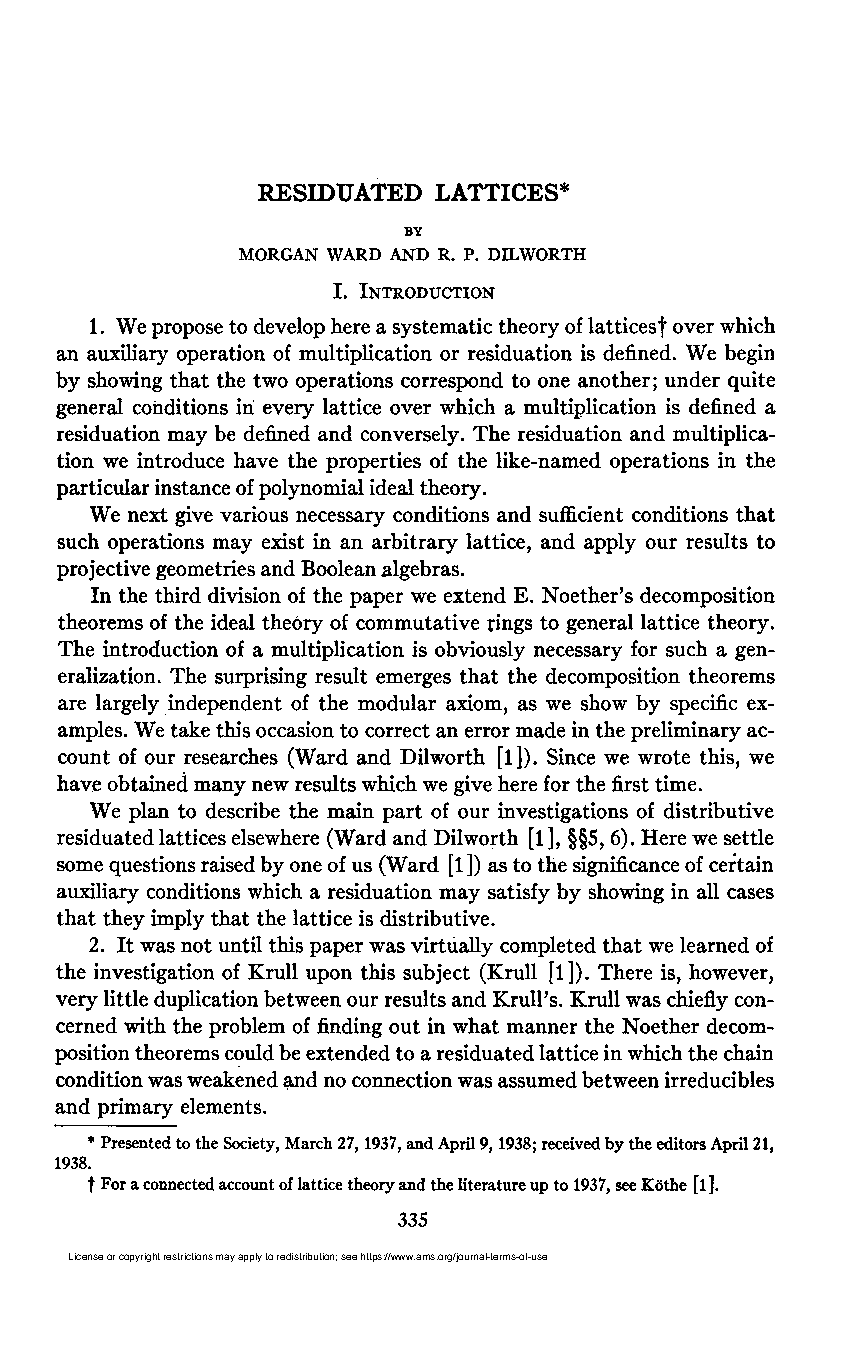
\includepdf[pages={-}]{1938-02 Residuated Lattices.pdf}
	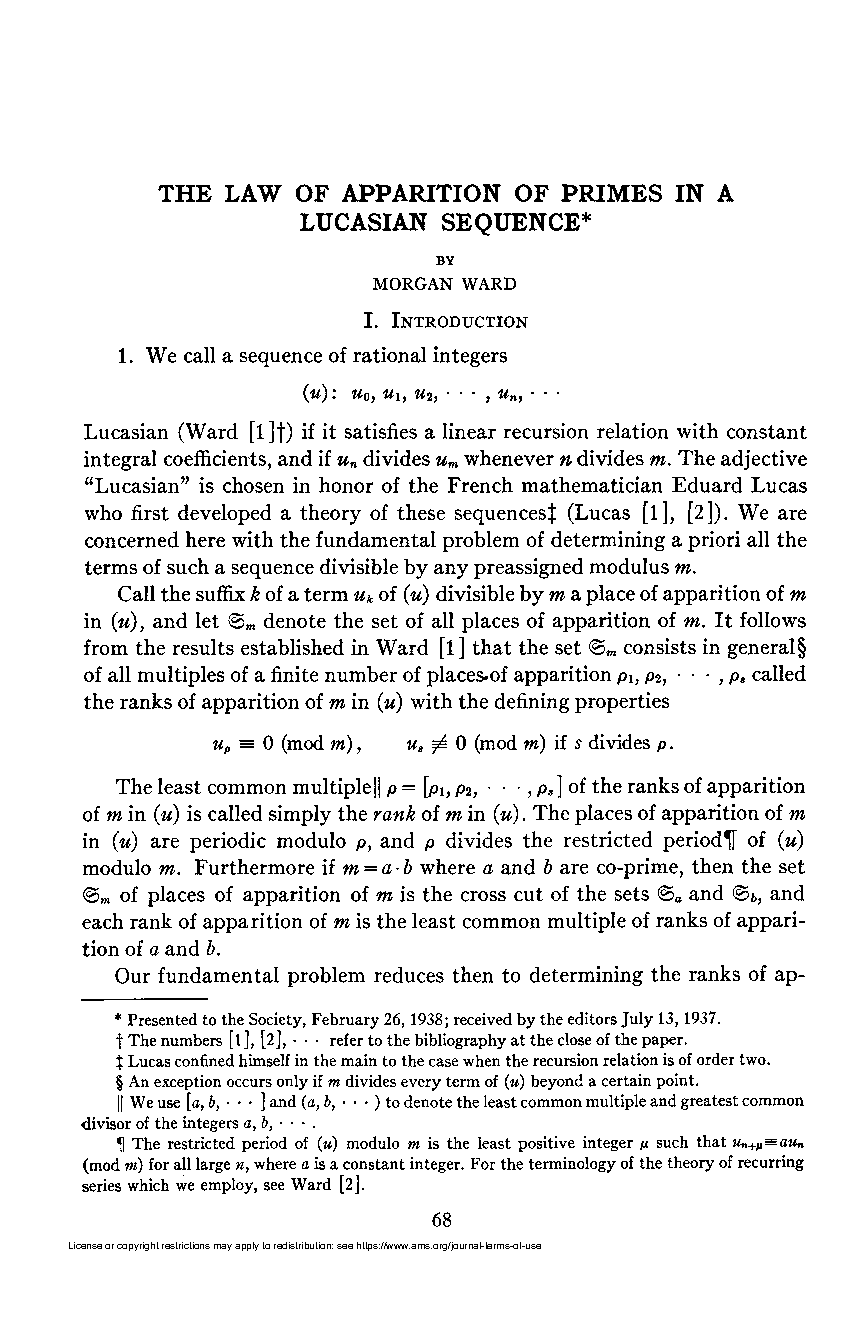
\includepdf[pages={-}]{1938-03 The Law of Apparition of Primes in a Lucasian Sequence.pdf}
	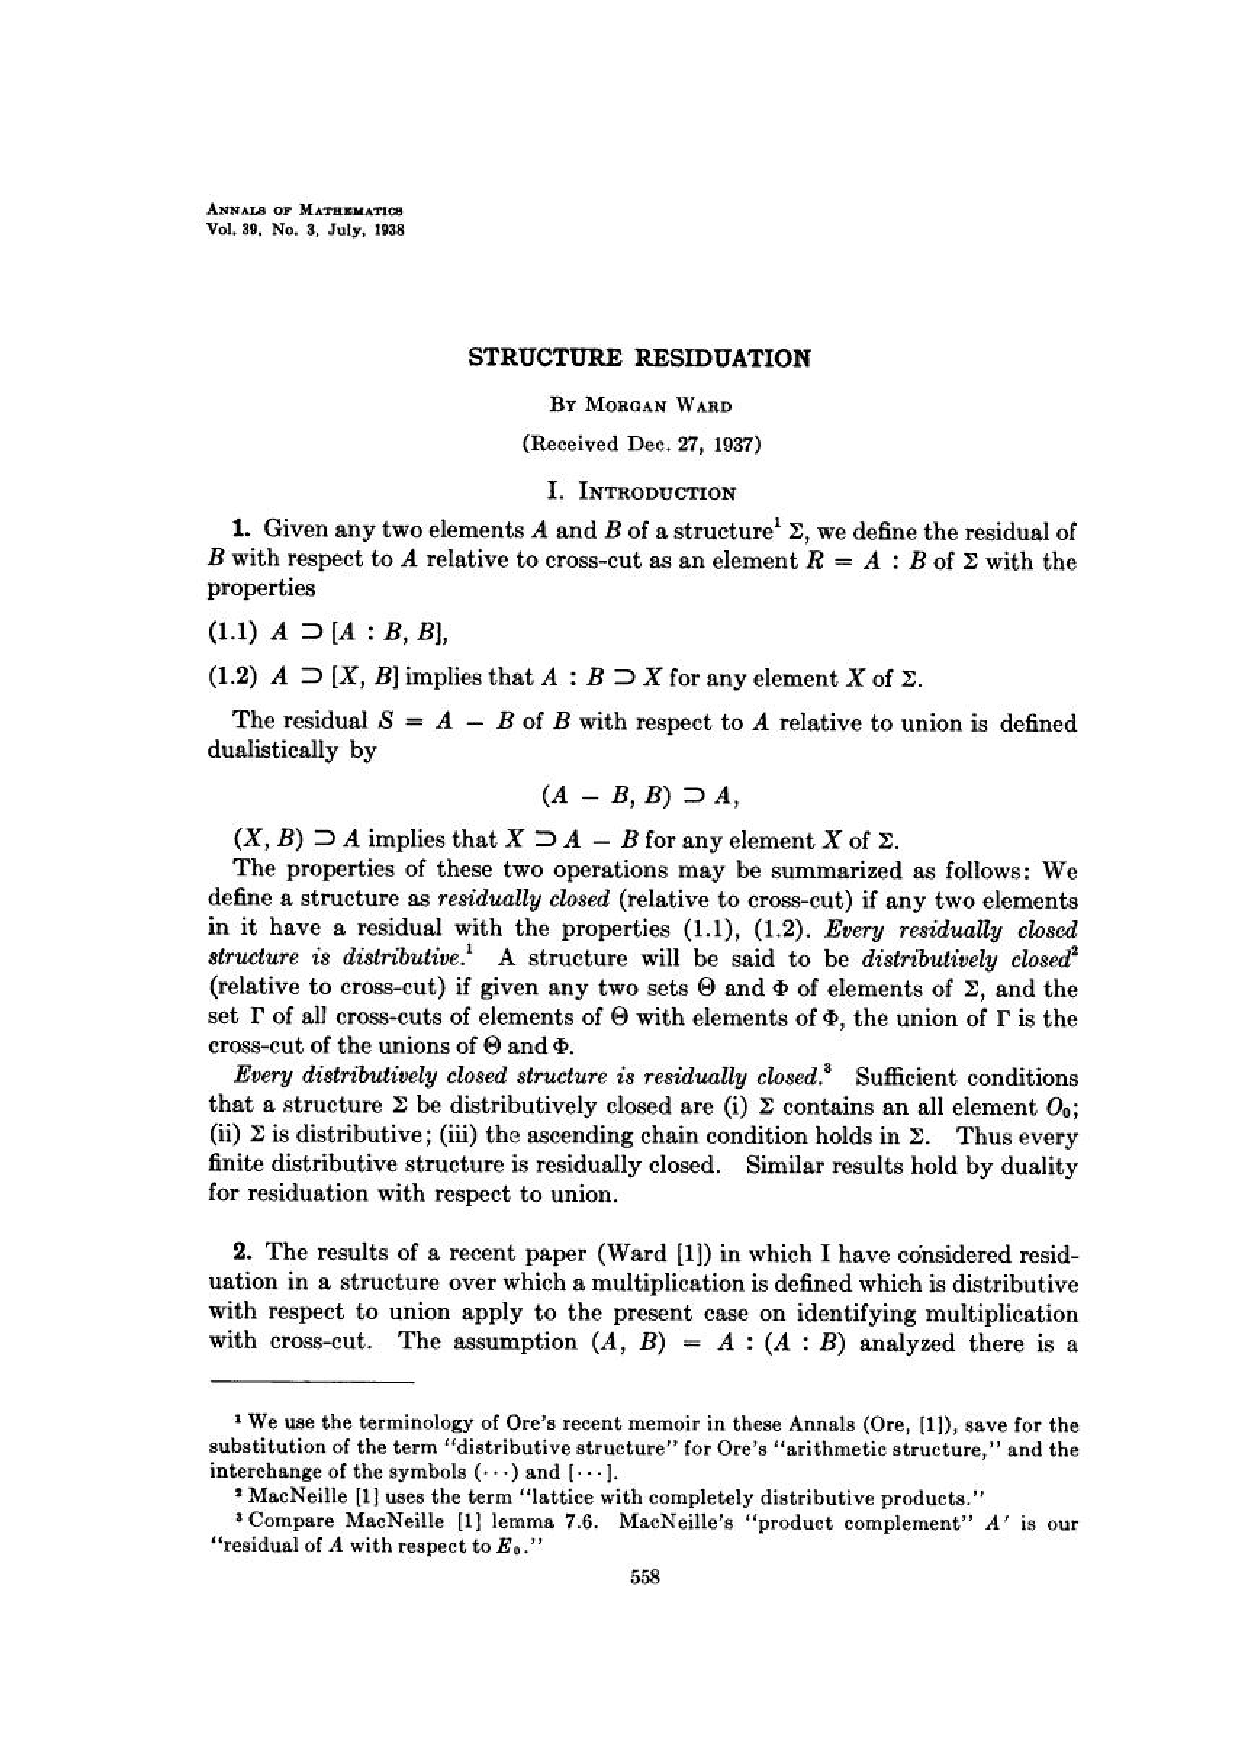
\includepdf[pages={-}]{1938-04 Structure Residuation.pdf}
	\chapter{1939}
	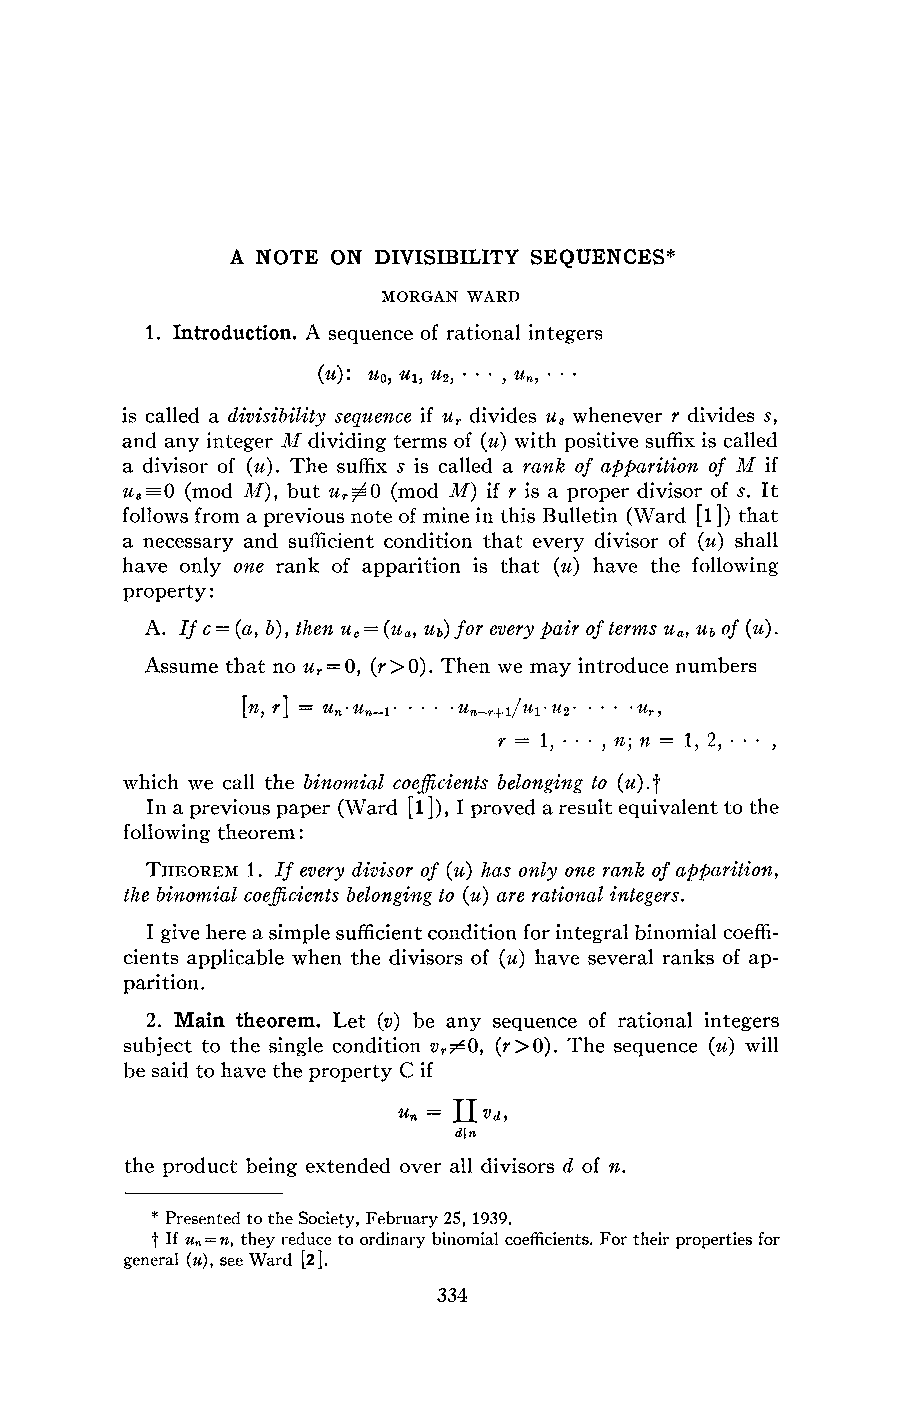
\includepdf[pages={-}]{1939-01 A note on divisibility sequences.pdf}
	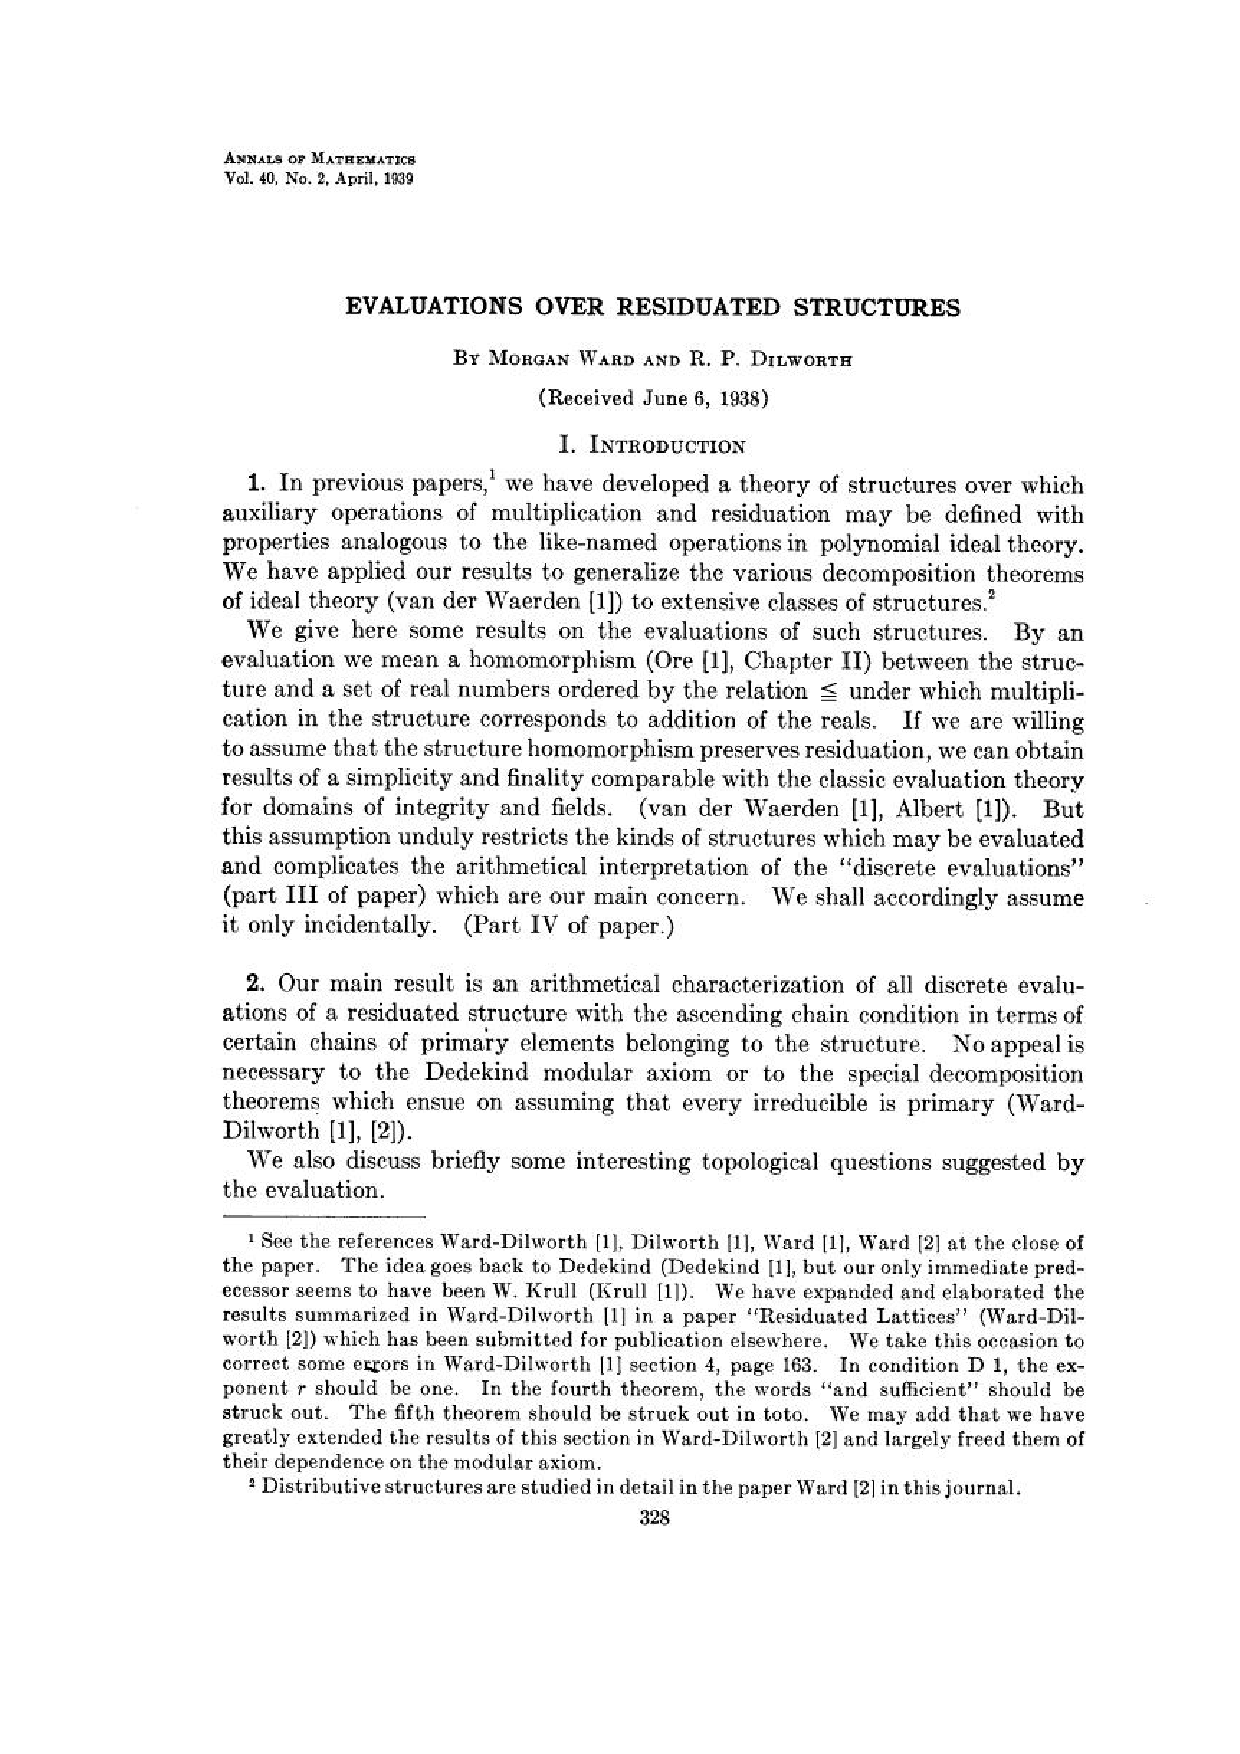
\includepdf[pages={-}]{1939-02 Evaluations Over Residuated Structures.pdf}
	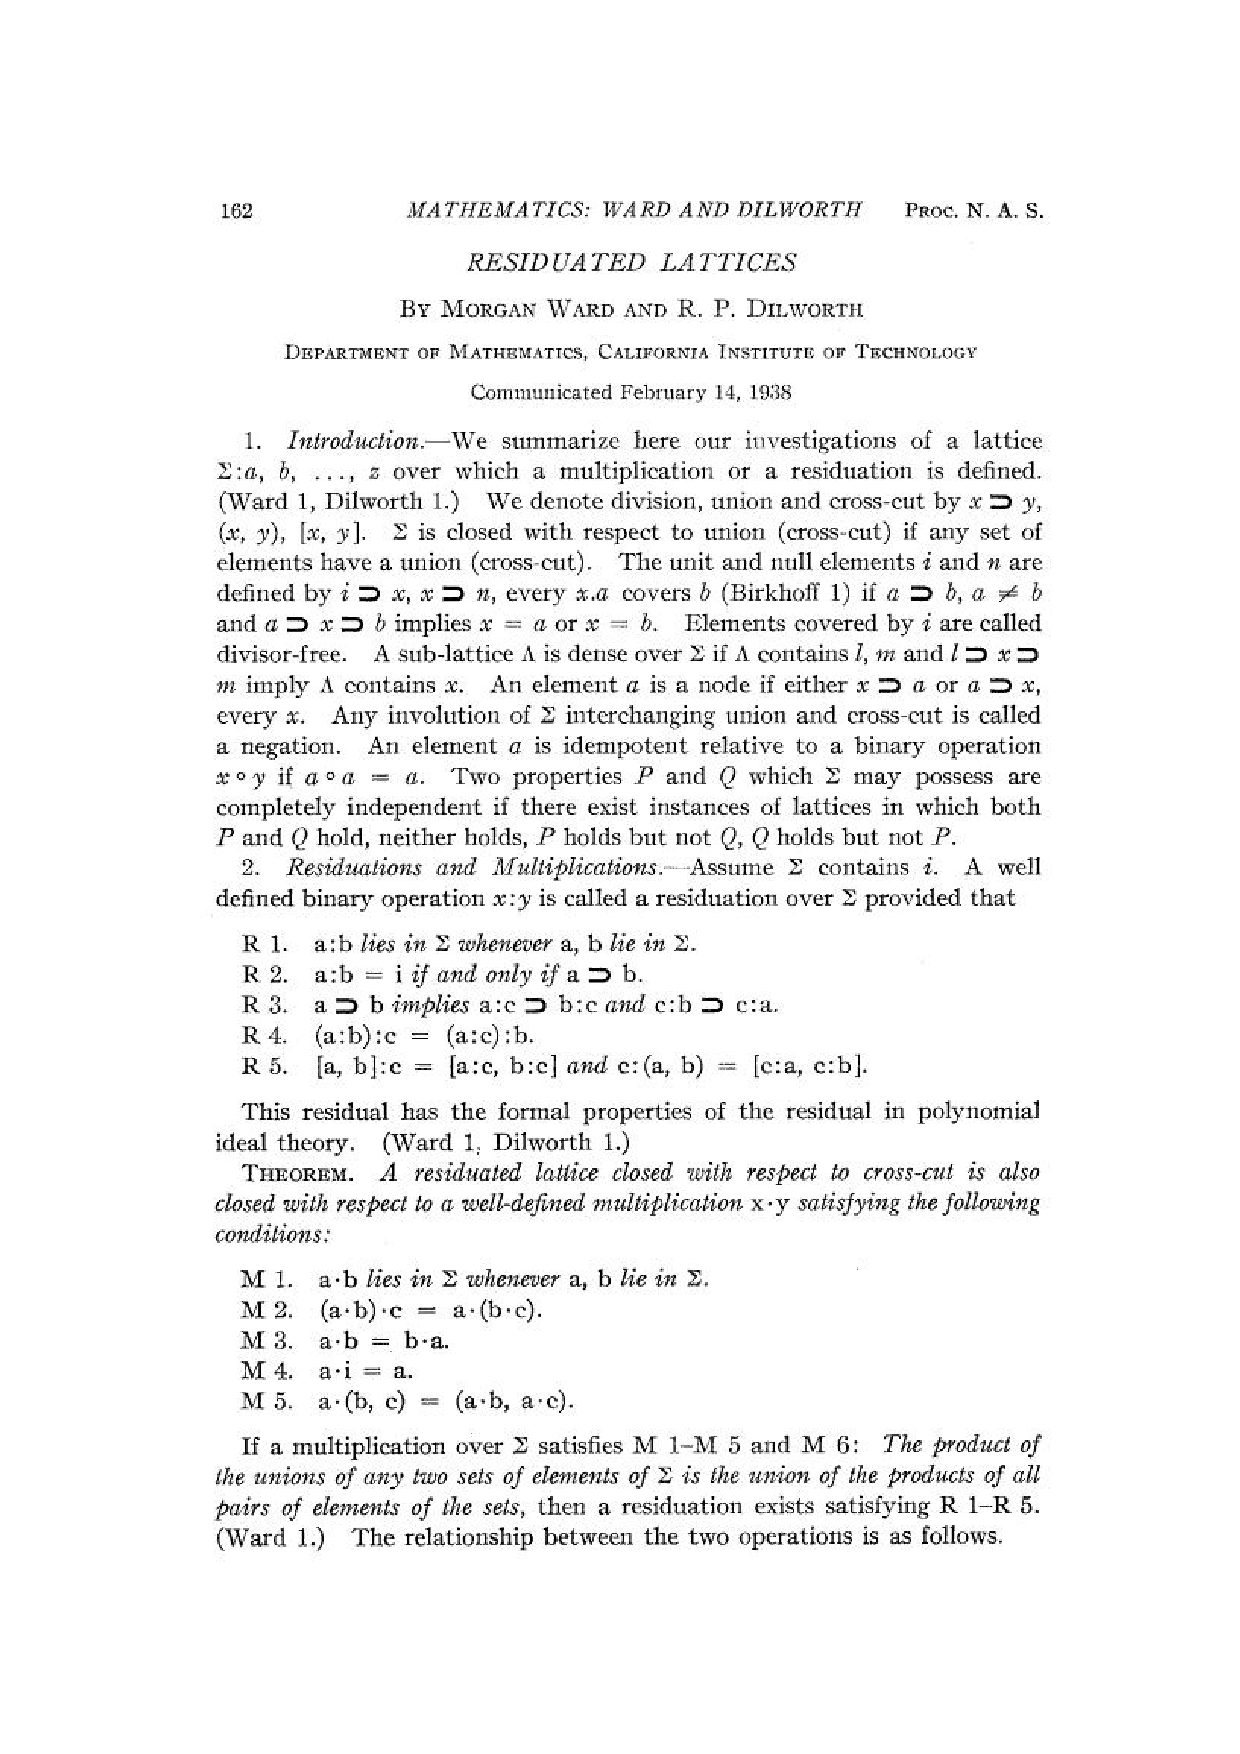
\includepdf[pages={-}]{1939-03 Residuated Lattices.pdf}
	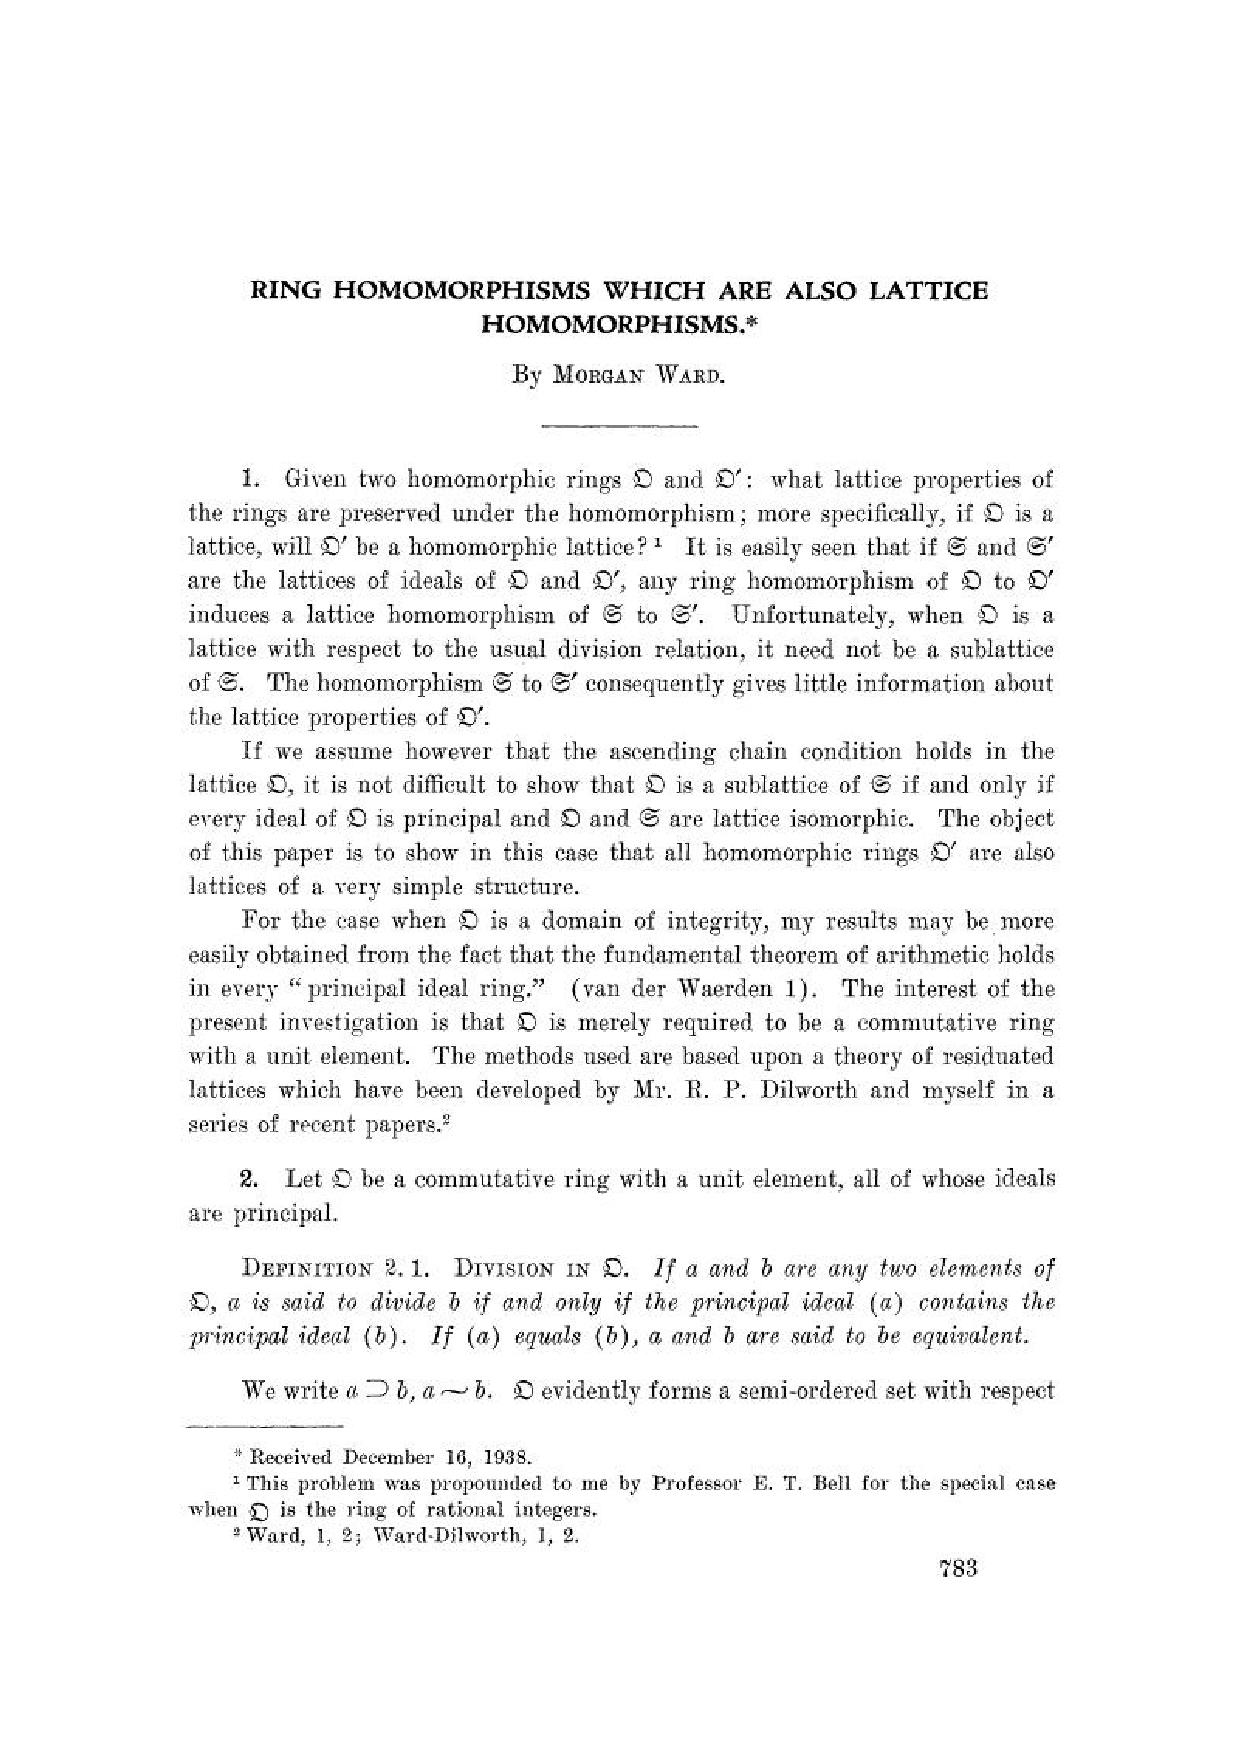
\includepdf[pages={-}]{1939-05 Ring Homomorphisms which are Also Lattice Homomorphisms.pdf}
	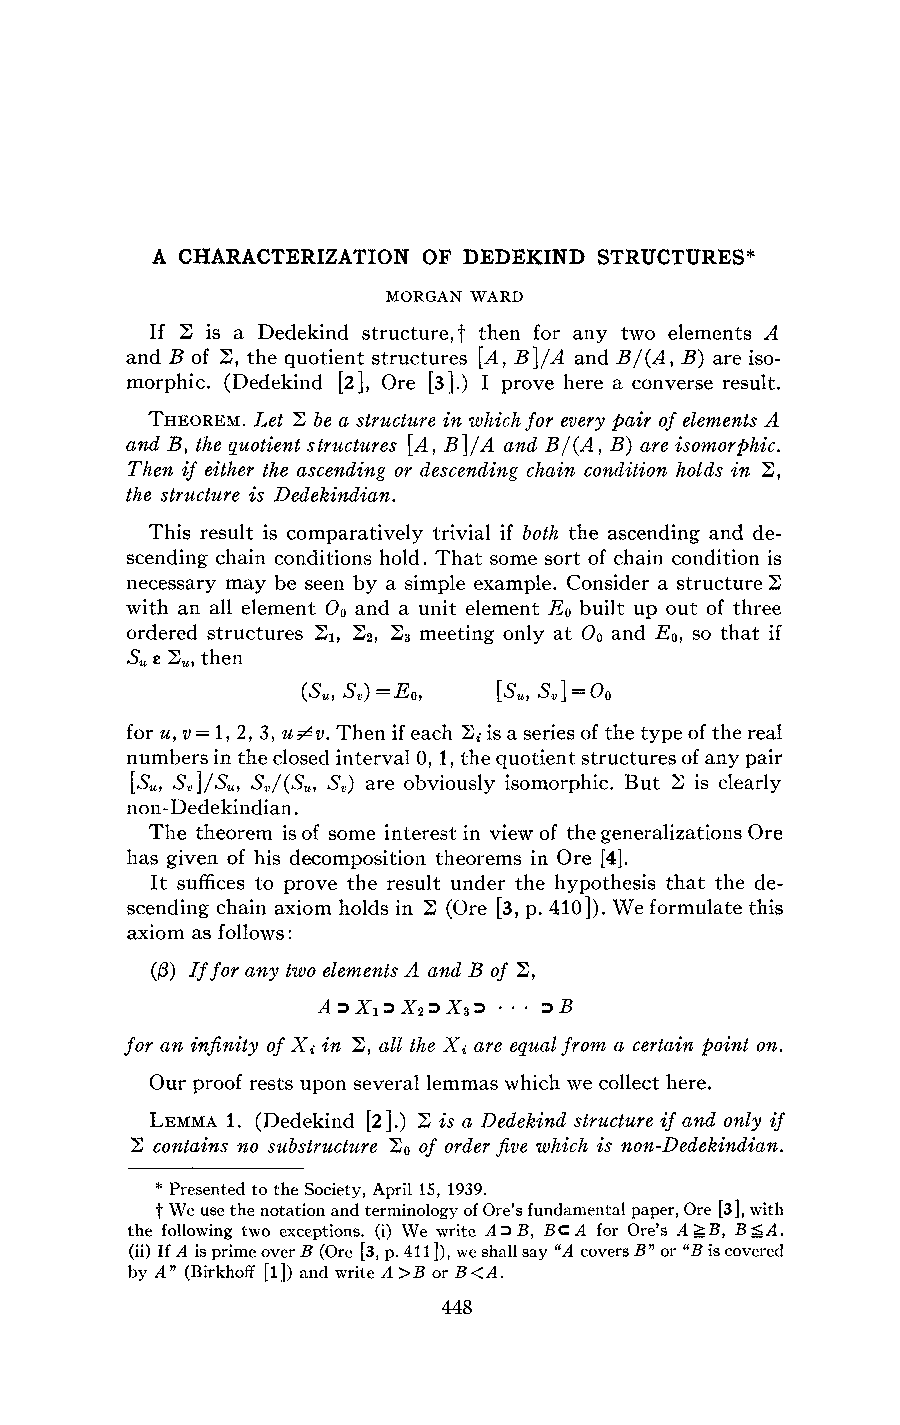
\includepdf[pages={-}]{1939-06 A characterization of Dedekind structures.pdf}
	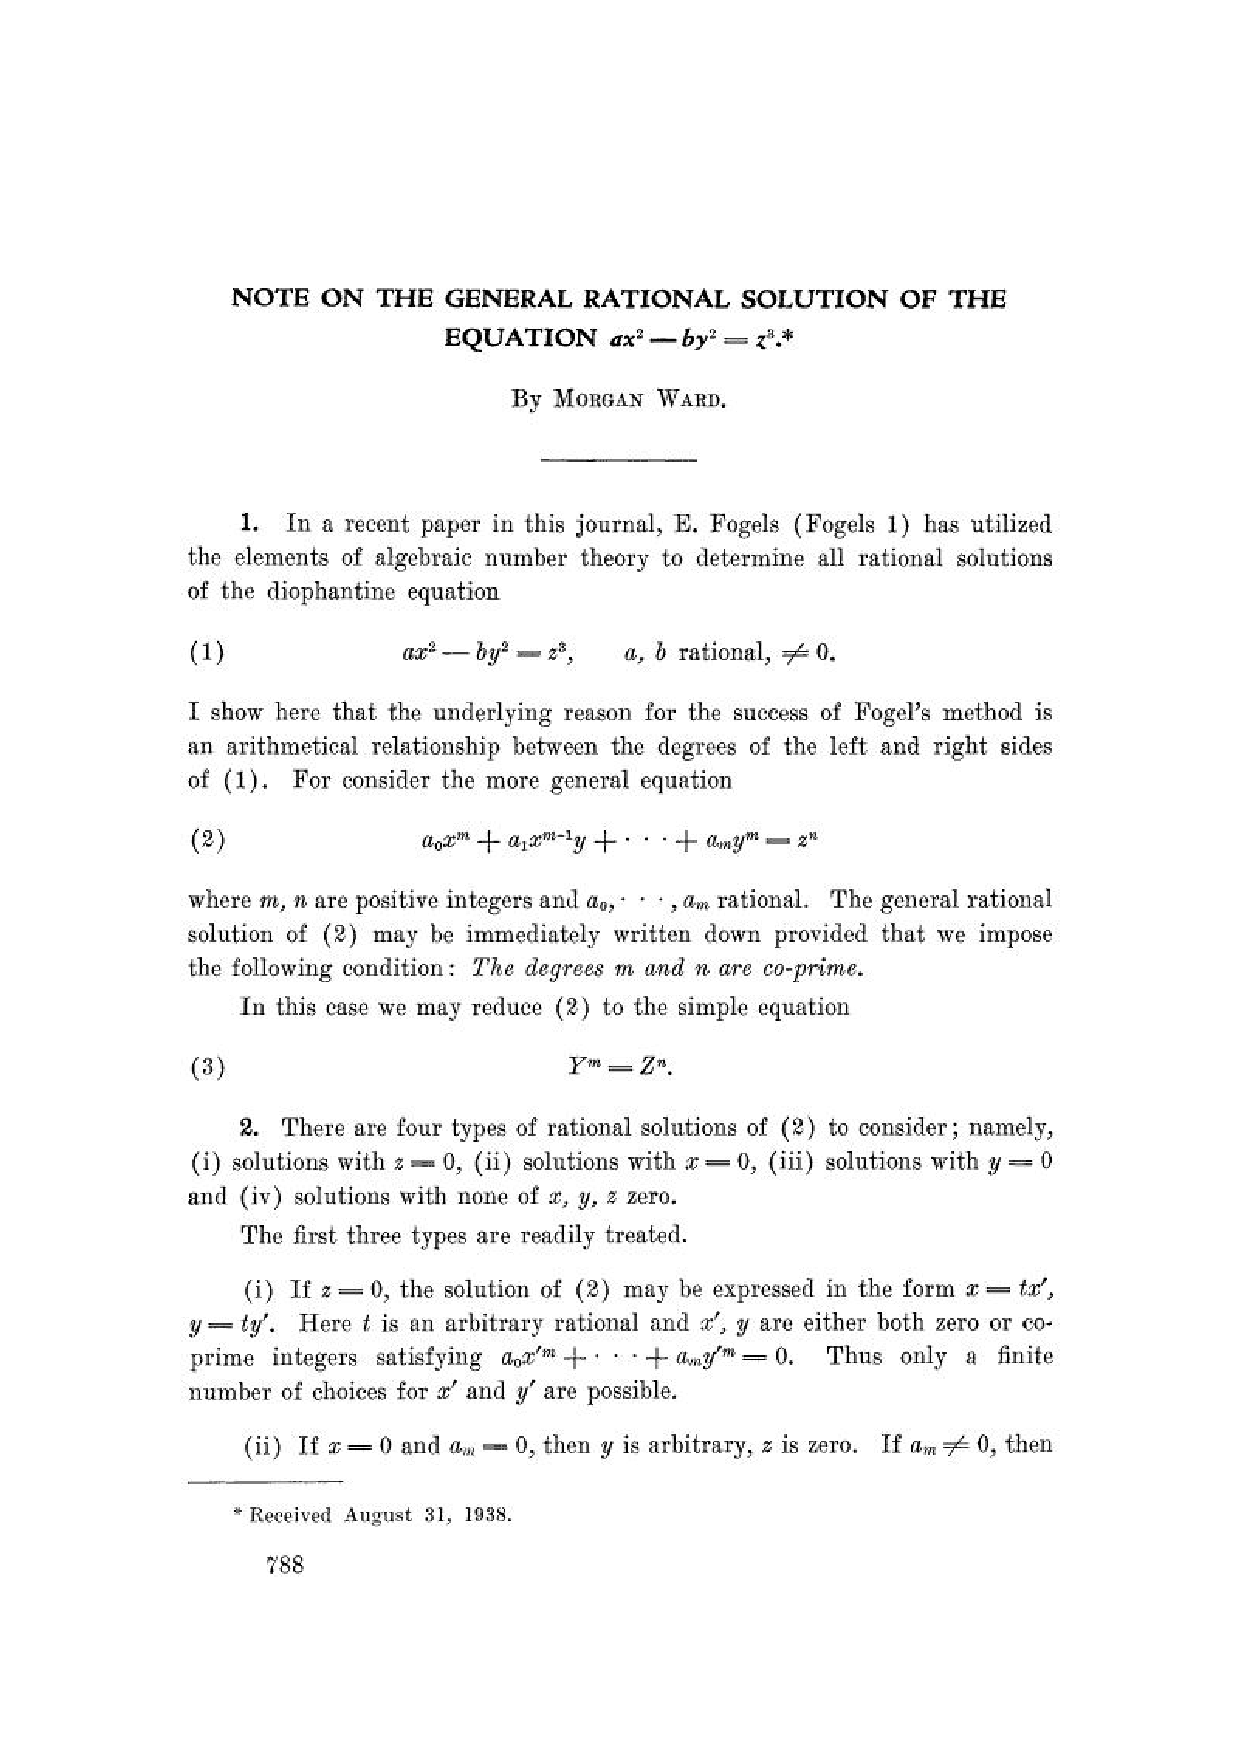
\includepdf[pages={-}]{1939-07 Note on the General Rational Solution of the Equation ax2 - by2 = z3.pdf}
	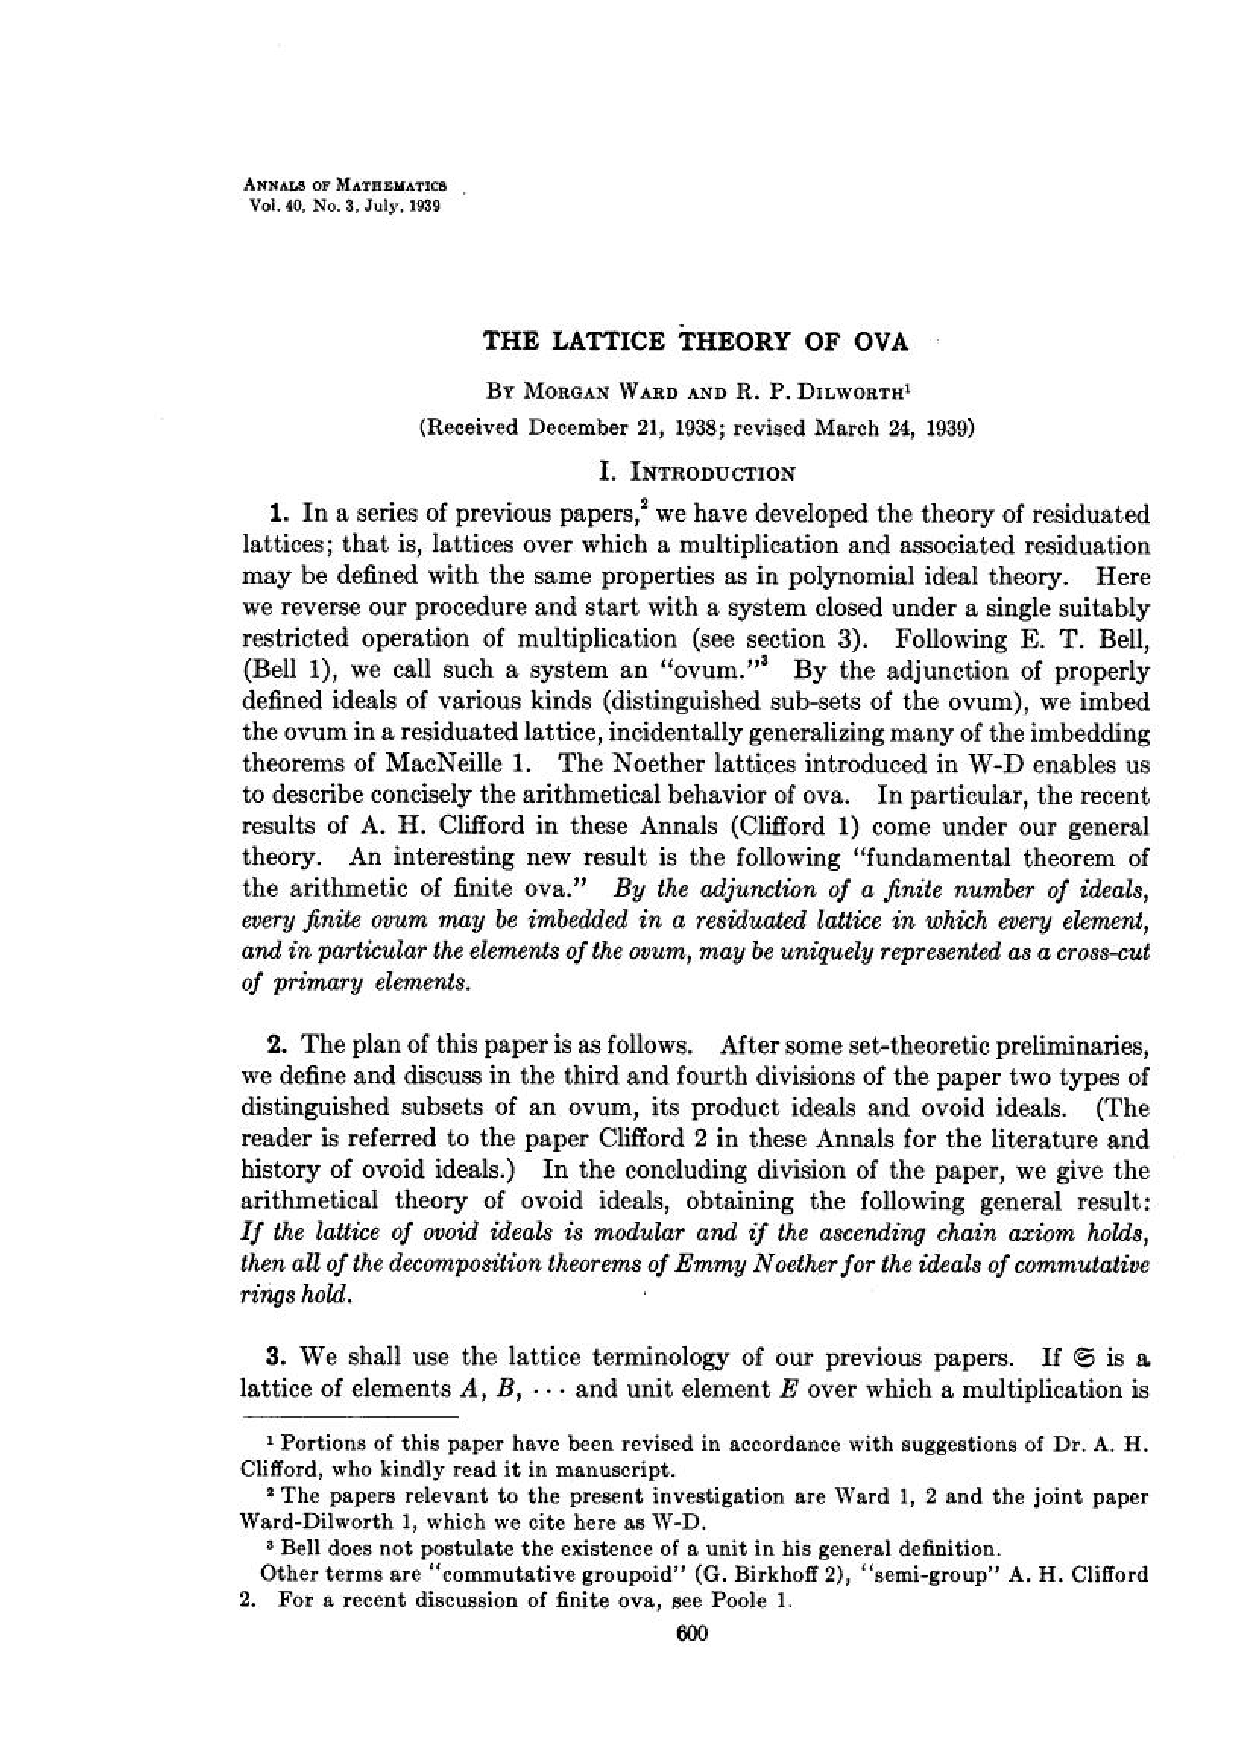
\includepdf[pages={-}]{1939-08 The Lattice Theory of Ova.pdf}
	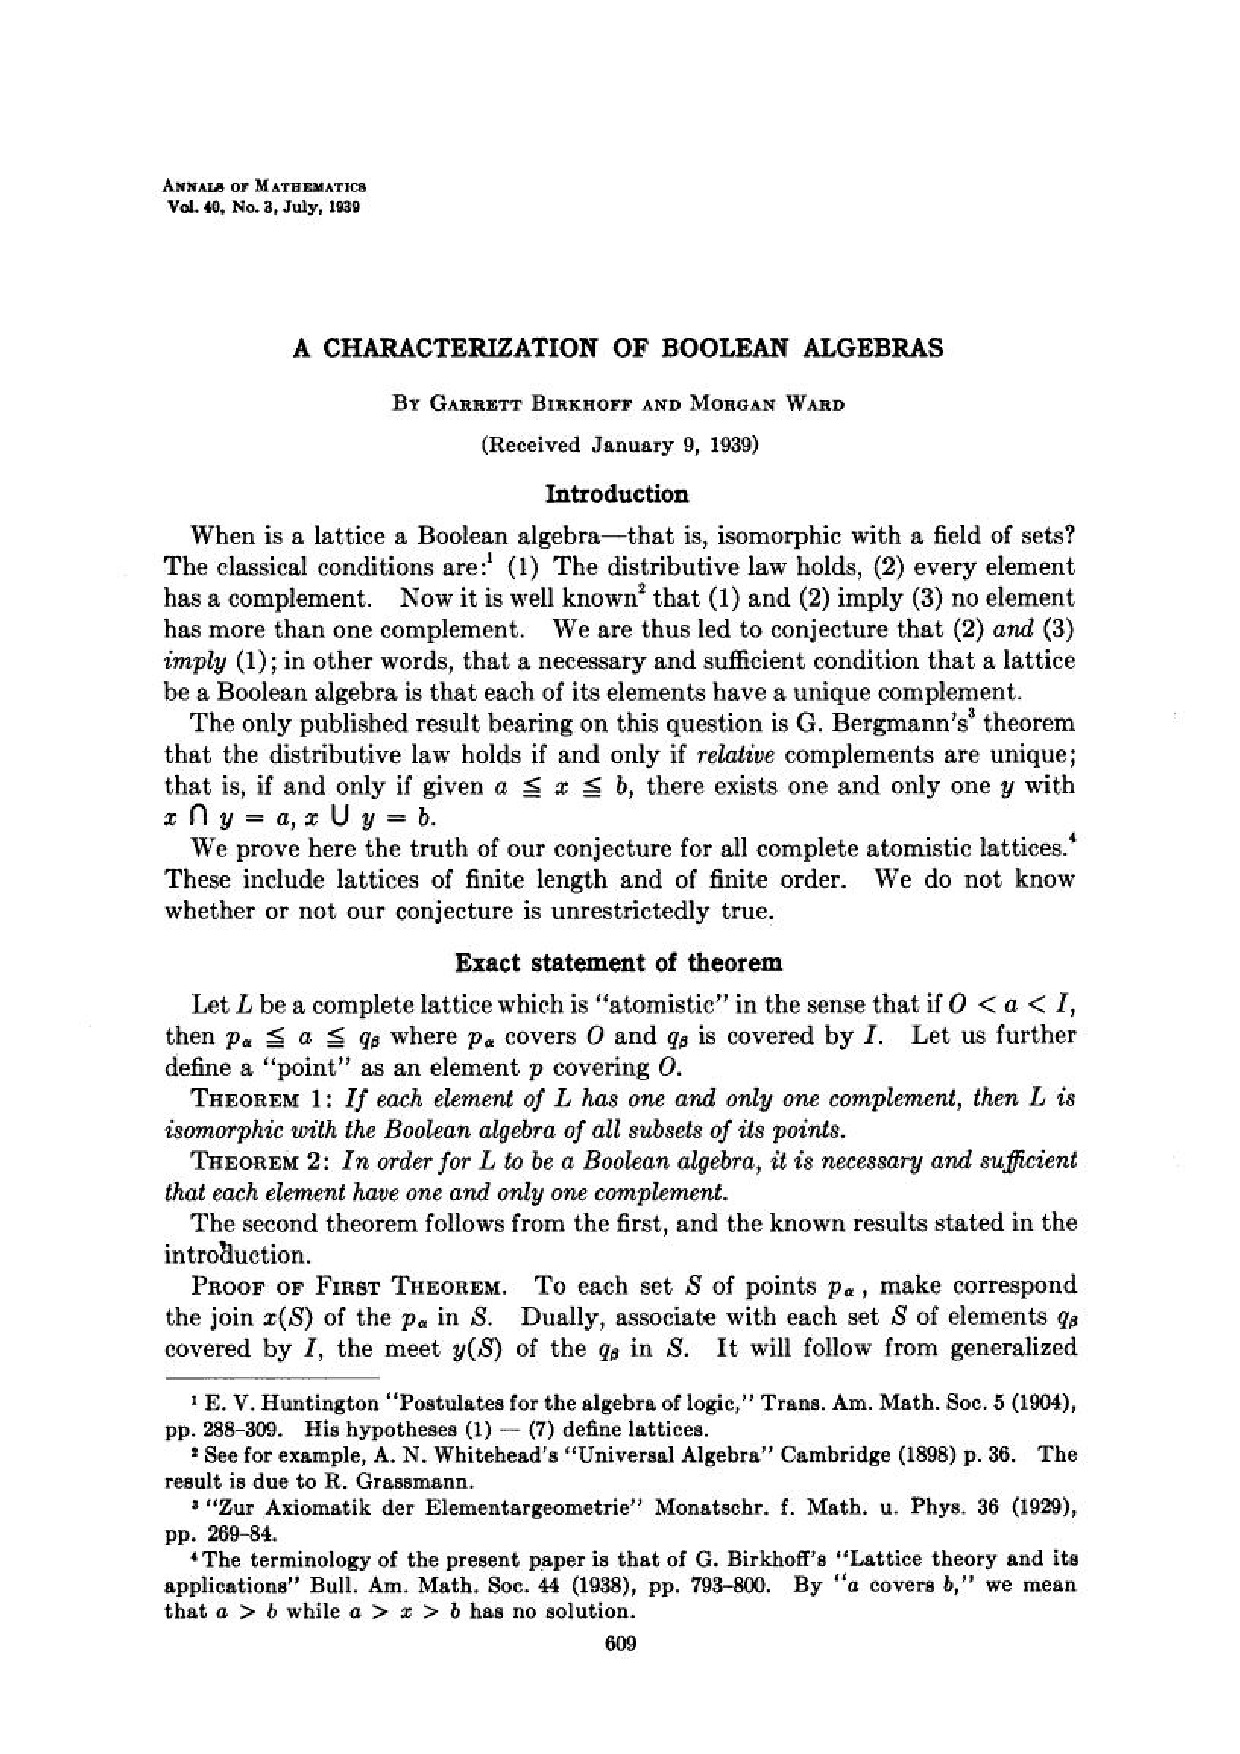
\includepdf[pages={-}]{1939-09 A Characterization of Boolean Algebras.pdf}
	\chapter{1942}
	\includepdf[pages={-}]{1942-01 The Closure Operators of a Lattice.pdf}
	\chapter{1945}
	\includepdf[pages={-}]{1945-01 Eulers three biquadrate problem.pdf}
	\chapter{1948}
	\includepdf[pages={-}]{1948-01 Memoir on Elliptic Divisibility Sequences.pdf}
	\chapter{1949}
	\includepdf[pages={-}]{1949-01 A Generalized Integral Test for Convergence of Series.pdf}
	\includepdf[pages={-}]{1949-02 Note on a paper by C E Rickart.pdf}
	\chapter{1950}
	\includepdf[pages={-}]{1950-01 Arithmetical Properties of the Elliptic Polynomials Arising from the Real Multiplication of the Jacobi Functions.pdf}
	\includepdf[pages={-}]{1950-02 Arithmetical properties of polynomials associated with the lemniscate elliptic functions.pdf}
	\chapter{1951}
	\includepdf[pages={-}]{1951-01 A class of soluble Diophantine equations.pdf}
	\chapter{1954}
	\includepdf[pages={-}]{1954-02 The maximal prime divisors of linear recurrences.pdf}
	\includepdf[pages={-}]{1954-03 Cyclotomy and the Converse of Fermat's Theorem.pdf}
	\chapter{1955}
	\includepdf[pages={-}]{1955-01 The Intrinsic Divisors of Lehmer Numbers.pdf}
	\includepdf[pages={-}]{1955-02 On the Number of Vanishing Terms in an Integral Cubic Recurrence.pdf}
	\includepdf[pages={-}]{1955-03 The laws of apparition and repetition of primes in a cubic recurrence.pdf}
	\includepdf[pages={-}]{1955-04 The mappings of the positive integers into themselves which preserve division.pdf}
	\chapter{1959}
	\includepdf[pages={-}]{1959-01 Testsfor primality based on Sylvester's cyclotomic numbers.pdf}
	\chapter{1960}
	\includepdf[pages={-}]{1960-02 The Calculation of the Complete Elliptic Integral of the Third Kind.pdf}
	\chapter{1961}
	\includepdf[pages={-}]{1961-01 The prime divisors of Fibonacci numbers.pdf}
	\chapter{1962}
	\includepdf[pages={-}]{1962-01 The linear p-adic recurrence of order two.pdf}
	
	\backmatter
	\begin{thebibliography}{99}
		\bibitem{lehmer} Lehmer, D. (1993). \textit{The Mathematical Work of Morgan Ward}. Mathematics of Computation, 61(203), 307-311.
	\end{thebibliography}
\end{document}